\documentclass[a4paper,12pt]{report}

% Citation en début de chapitre
\usepackage{epigraph}

% Encodages et langue (XeLaTeX/LuaLaTeX natif UTF-8)
\usepackage{iftex}
\ifPDFTeX
  \usepackage[utf8]{inputenc}
  \usepackage[T1]{fontenc}
\else
  \usepackage{fontspec}
\fi
\usepackage[french]{babel}
\usepackage{csquotes}

\usepackage[backend=biber]{biblatex}
\addbibresource{references.bib}
\usepackage{libertine}
\usepackage{setspace}          % Added for \setstretch
\usepackage{tabularx}

% Mise en page
\usepackage[margin=2.5cm, headheight=15pt]{geometry} % Marges du document

% Python 
\usepackage{pythonhighlight}

\usepackage{fancybox} % Pour créer des cadres élégants


% Inclusion d'images
\usepackage{graphicx}          % Pour inclure des images

% Ajout du package float pour le positionnement [H]
\usepackage{float}

% Bibliothèques pour les mathématiques
\usepackage{amsmath} % Mathématiques avancées
\usepackage{amssymb} % Symboles mathématiques
\usepackage{amsfonts} % Polices mathématiques
\usepackage{amsthm} % Définitions et théorèmes
\usepackage{algorithm}
\usepackage{algpseudocode}
\usepackage{tikz}
\usepackage{pgfplots}
\pgfplotsset{compat=1.18}
\usepackage{amsmath, amsthm}
% Configuration des définitions et théorèmes
\newtheorem{definition}{Définition}[chapter] % Définitions numérotées par chapitre
\newtheorem{theorem}{Théorème}[chapter] % Théorèmes numérotés par chapitre
\newtheorem{example}{Exemple}[chapter] % Exemples numérotés par chapitre
\newtheorem{remark}{Remarque}[chapter] % Remarques numérotées par chapitre


\usepackage{xcolor}
\definecolor{grey}{rgb}{0.5, 0.5, 0.5} % Définit la couleur grey

% Couleurs personnalisées pour la page de garde
\definecolor{burgundy}{HTML}{8e5e2d} % Couleur principale #4b0e20
\definecolor{gold}{HTML}{4c1207} % Couleur secondaire #b29959

% Configuration des couleurs pour les sections, sous-sections, etc.
\usepackage{titlesec}
\usepackage{subcaption}
\usepackage{svg}
\usepackage{wrapfig}


% Personnalisation des titres de section en burgundy
\titleformat{\section}
  {\Large\bfseries\color{burgundy}}
  {\thesection}
  {1em}
  {}

\titleformat{\subsection}
  {\large\bfseries\color{burgundy}}
  {\thesubsection}
  {1em}
  {}

\titleformat{\subsubsection}
  {\normalsize\bfseries\color{burgundy}}
  {\thesubsubsection}
  {1em}
  {}

% Hyperliens
\usepackage{hyperref}
\hypersetup{
    colorlinks=true,            % Colore les liens
    linkcolor=burgundy,         % Couleur des liens internes (ex. table des matières) - burgundy
    citecolor=gold,             % Couleur des références bibliographiques - gold
    filecolor=burgundy,         % Couleur des liens vers des fichiers locaux - burgundy
    urlcolor=gold               % Couleur des URL - gold
}




\usepackage{enumitem}
\usepackage{booktabs}
\usepackage{multirow}
\usepackage{siunitx}
\usepackage{subcaption}

% En-têtes et pieds de page
\usepackage{fancyhdr}          % Pour personnaliser les en-têtes et pieds de page
\usepackage{lastpage}          % Pour référencer la dernière page

% Configuration du package fancyhdr
\pagestyle{fancy}
\fancyhf{} % Efface tous les champs de l'en-tête et du pied de page

% En-tête
\lhead{\textbf{\color{burgundy}CHPS0701 : Algorithmique et Programmation Parallèle}} % En-tête à gauche
\rhead{\textbf{\color{burgundy}M1 CHPS}} % En-tête à droite

% Pied de page
\lfoot{\textbf{\color{burgundy}Romain Despoullains}} % Pied de page à gauche
\rfoot{\textbf{\color{burgundy}Page \thepage\ \color{burgundy}/ \color{burgundy}\pageref{LastPage}}} % Pied de page à droite

% --- Personnalisation des lignes d'en-tête et de pied de page ---
\renewcommand{\headrulewidth}{0.4pt} % Épaisseur de la ligne sous l'en-tête
\renewcommand{\footrulewidth}{0.4pt} % Épaisseur de la ligne au-dessus du pied de page

% Redéfinition de \headrule et \footrule pour changer leur couleur
% On utilise \fancy@setcolor pour que la couleur soit correctement gérée par fancyhdr
\makeatletter % Nécessaire pour utiliser des commandes avec @

% Pour la ligne d'en-tête
\renewcommand{\headrule}{%
  \if@fancyplain\let\headrulewidth\plainheadrulewidth\fi
  {\color{burgundy} % Définit la couleur de la règle
  \hrule\@width\headwidth\@height\headrulewidth\vskip-\headrulewidth}
  \if@fancyplain\let\headrulewidth\plainheadrulewidth\fi % Rétablit la valeur originale (important)
}

% Pour la ligne de pied de page
\renewcommand{\footrule}{%
  \if@fancyplain\let\footrulewidth\plainfootrulewidth\fi
  \vskip-\footruleskip\vskip-\footrulewidth
  {\color{burgundy} % Définit la couleur de la règle
  \hrule\@width\headwidth\@height\footrulewidth\vskip\footruleskip} % Utilise \headwidth pour la largeur
  \if@fancyplain\let\footrulewidth\plainfootrulewidth\fi % Rétablit la valeur originale
}
\makeatother
% Ajouter les lignes sous l'en-tête et au-dessus du pied de page
\renewcommand{\headrulewidth}{0.4pt} % Ligne sous l'en-tête
\renewcommand{\footrulewidth}{0.4pt} % Ligne au-dessus du pied de page

% Inclusion de code source (si nécessaire)
\usepackage{listings}      % Inclusion de code source
\usepackage{color}         % Couleurs


\definecolor{lightgray}{gray}{0.95}
\definecolor{darkgray}{gray}{0.4}
\definecolor{purple}{rgb}{0.58,0,0.82}

\lstdefinelanguage{bash}{
  keywords={cd, ls, mkdir, rm, mv, cp, sudo, apt, grep, find, echo, cat, git, docker, cargo},
  sensitive=true,
  comment=[l]{\#},
  morecomment=[l]{\#},
  morestring=[b]",
}

\lstset{
  language=bash,
  basicstyle=\small\ttfamily,
  backgroundcolor=\color{lightgray},
  commentstyle=\color{darkgray}\itshape,
  keywordstyle=\color{purple}\bfseries,
  stringstyle=\color{blue},
  breaklines=true,
  breakatwhitespace=true,
  frame=single,
  showstringspaces=false,
  tabsize=2,
  captionpos=b,
  extendedchars=true,
  literate=
    {├}{{\char"251C}}1
    {─}{{\char"2500}}1
    {└}{{\char"2514}}1
    {│}{{\char"2502}}1
}


% Définition des couleurs pour la coloration syntaxique
\definecolor{dkgreen}{rgb}{0,0.6,0}
\definecolor{gray}{rgb}{0.5,0.5,0.5}
\definecolor{mauve}{rgb}{0.58,0,0.82}

% Configuration du package listings
\definecolor{maroon}{cmyk}{0, 0.87, 0.68, 0.32}
\definecolor{halfgray}{gray}{0.55}
\definecolor{ipython_frame}{RGB}{207, 207, 207}
\definecolor{ipython_bg}{RGB}{247, 247, 247}
\definecolor{ipython_red}{RGB}{186, 33, 33}
\definecolor{ipython_green}{RGB}{0, 128, 0}
\definecolor{ipython_cyan}{RGB}{64, 128, 128}
\definecolor{ipython_purple}{RGB}{170, 34, 255}

\usepackage{listings}
\lstset{
    breaklines=true,
    %
    extendedchars=true,
    literate=
    {á}{{\'a}}1 {é}{{\'e}}1 {í}{{\'i}}1 {ó}{{\'o}}1 {ú}{{\'u}}1
    {Á}{{\'A}}1 {É}{{\'E}}1 {Í}{{\'I}}1 {Ó}{{\'O}}1 {Ú}{{\'U}}1
    {à}{{\`a}}1 {è}{{\`e}}1 {ì}{{\`i}}1 {ò}{{\`o}}1 {ù}{{\`u}}1
    {À}{{\`A}}1 {È}{{\'E}}1 {Ì}{{\`I}}1 {Ò}{{\`O}}1 {Ù}{{\`U}}1
    {ä}{{\"a}}1 {ë}{{\"e}}1 {ï}{{\"i}}1 {ö}{{\"o}}1 {ü}{{\"u}}1
    {Ä}{{\"A}}1 {Ë}{{\"E}}1 {Ï}{{\"I}}1 {Ö}{{\"O}}1 {Ü}{{\"U}}1
    {â}{{\^a}}1 {ê}{{\^e}}1 {î}{{\^i}}1 {ô}{{\^o}}1 {û}{{\^u}}1
    {Â}{{\^A}}1 {Ê}{{\^E}}1 {Î}{{\^I}}1 {Ô}{{\^O}}1 {Û}{{\^U}}1
    {œ}{{\oe}}1 {Œ}{{\OE}}1 {æ}{{\ae}}1 {Æ}{{\AE}}1 {ß}{{\ss}}1
    {ç}{{\c c}}1 {Ç}{{\c C}}1 {ø}{{\o}}1 {å}{{\r a}}1 {Å}{{\r A}}1
    {€}{{\EUR}}1 {£}{{\pounds}}1,
    %
    literate=
    *{+}{{{\color{ipython_purple}+}}}1
    {-}{{{\color{ipython_purple}-}}}1
    {*}{{{\color{ipython_purple}$^\ast$}}}1
    {/}{{{\color{ipython_purple}/}}}1
    {^}{{{\color{ipython_purple}\^{}}}}1
    {?}{{{\color{ipython_purple}?}}}1
    {!}{{{\color{ipython_purple}!}}}1
    {\%}{{{\color{ipython_purple}\%}}}1
    {<}{{{\color{ipython_purple}<}}}1
    {>}{{{\color{ipython_purple}>}}}1
    {|}{{{\color{ipython_purple}|}}}1
    {\&}{{{\color{ipython_purple}\&}}}1
    {~}{{{\color{ipython_purple}\char126}}}1
    %
    {==}{{{\color{ipython_purple}==}}}2
    {<=}{{{\color{ipython_purple}<=}}}2
    {>=}{{{\color{ipython_purple}>=}}}2
    %
    {+=}{{{+=}}}2
    {-=}{{{-=}}}2
    {*=}{{{$^\ast$=}}}2
    {/=}{{{/=}}}2,
    %
%   identifierstyle=\color{red}\ttfamily,
    commentstyle=\color{ipython_cyan}\ttfamily,
    stringstyle=\color{ipython_red}\ttfamily,
    keepspaces=true,
    showspaces=false,
    showstringspaces=false,
    %
    rulecolor=\color{ipython_frame},
    frame=single,
    frameround={t}{t}{t}{t},
    framexleftmargin=6mm,
    numbers=left,
    numberstyle=\tiny\color{halfgray},
    %
    %
    backgroundcolor=\color{ipython_bg},
    %   extendedchars=true,
    basicstyle=\scriptsize\ttfamily,
    keywordstyle=\color{ipython_green}\ttfamily,
    escapechar=@,
}


% Inclusion de PlantUML pour les schémas basiques
\usepackage{tikz}
\usetikzlibrary{shapes.geometric, arrows, positioning, calc, patterns, decorations.pathreplacing, matrix, fit, backgrounds}

% Command for horizontal rule on title page
\newcommand{\HRule}{\rule{\linewidth}{0.5mm}}

% Schema placeholder : standardised fbox describing where to paste a
% generated PNG. Usage : \schemaImage{caption description}.
\newcommand{\schemaImage}[1]{%
  \fbox{\parbox{0.85\textwidth}{\centering\small%
    [Schema PNG manquant.]\\[1ex]%
    \textbf{Sujet :} #1}}%
}

% Informations du document
\title{Cours}
\author{Université de Reims Champagne Ardennes \\ Despoullains Romain}
\date{\\today}

\usepackage{tcolorbox} % Pour les boîtes stylisées
\tcbuselibrary{breakable} % Pour permettre les boîtes sur plusieurs pages

\tcbset {
  base/.style={
    arc=0mm, 
    bottomtitle=0.5mm,
    boxrule=0mm,
    colbacktitle=black!10!white, 
    coltitle=black, 
    fonttitle=\bfseries, 
    left=2.5mm,
    leftrule=1mm,
    right=3.5mm,
    title={#1},
    toptitle=0.75mm, 
  }
}

% Définition des couleurs
\definecolor{brandblue}{rgb}{0.34, 0.7, 1}
\definecolor{brandgreen}{rgb}{0.0, 0.8, 0.4}
\definecolor{brandorange}{rgb}{1.0, 0.6, 0.0}
\definecolor{brandred}{rgb}{0.9, 0.1, 0.2}

\newtcolorbox{methode}[1]{
  colframe=brandblue, 
  base={#1}
}

\newtcolorbox{defi}[1]{
  colframe=brandgreen,
  base={#1}
}

\newtcolorbox{exemple}[1]{
  colframe=brandorange,
  base={#1}
}

\newtcolorbox{important}[1]{
  colframe=brandred,
  base={#1}
}

% Couleurs supplémentaires pour les encadrés
\definecolor{brandpurple}{rgb}{0.5, 0.0, 0.5}
\definecolor{brandteal}{rgb}{0.0, 0.5, 0.5}

% Encadré pour les résultats importants
\newtcolorbox{result}{
  colframe=brandpurple,
  colback=brandpurple!5,
  arc=2mm,
  boxrule=1pt,
  left=3mm,
  right=3mm,
  top=2mm,
  bottom=2mm,
  fonttitle=\bfseries,
  title={Résultat clé}
}

% Encadré pour les recommandations
\newtcolorbox{recommendation}{
  colframe=brandteal,
  colback=brandteal!5,
  arc=2mm,
  boxrule=1pt,
  left=3mm,
  right=3mm,
  top=2mm,
  bottom=2mm,
  fonttitle=\bfseries,
  title={Recommandation}
}

% Packages for background image and graphics
\usepackage{eso-pic}
\usepackage{graphicx}
\usepackage{tikz}
%-----------------------------------------------------------------
% Command to place a background image at 15% opacity
%-----------------------------------------------------------------
\newcommand\BackgroundPic{%
  \begin{tikzpicture}[remember picture,overlay]
    % The node has "opacity=0.15" to set the entire image at 15% visibility.
    \node[opacity=0.20] at (current page.center){%
      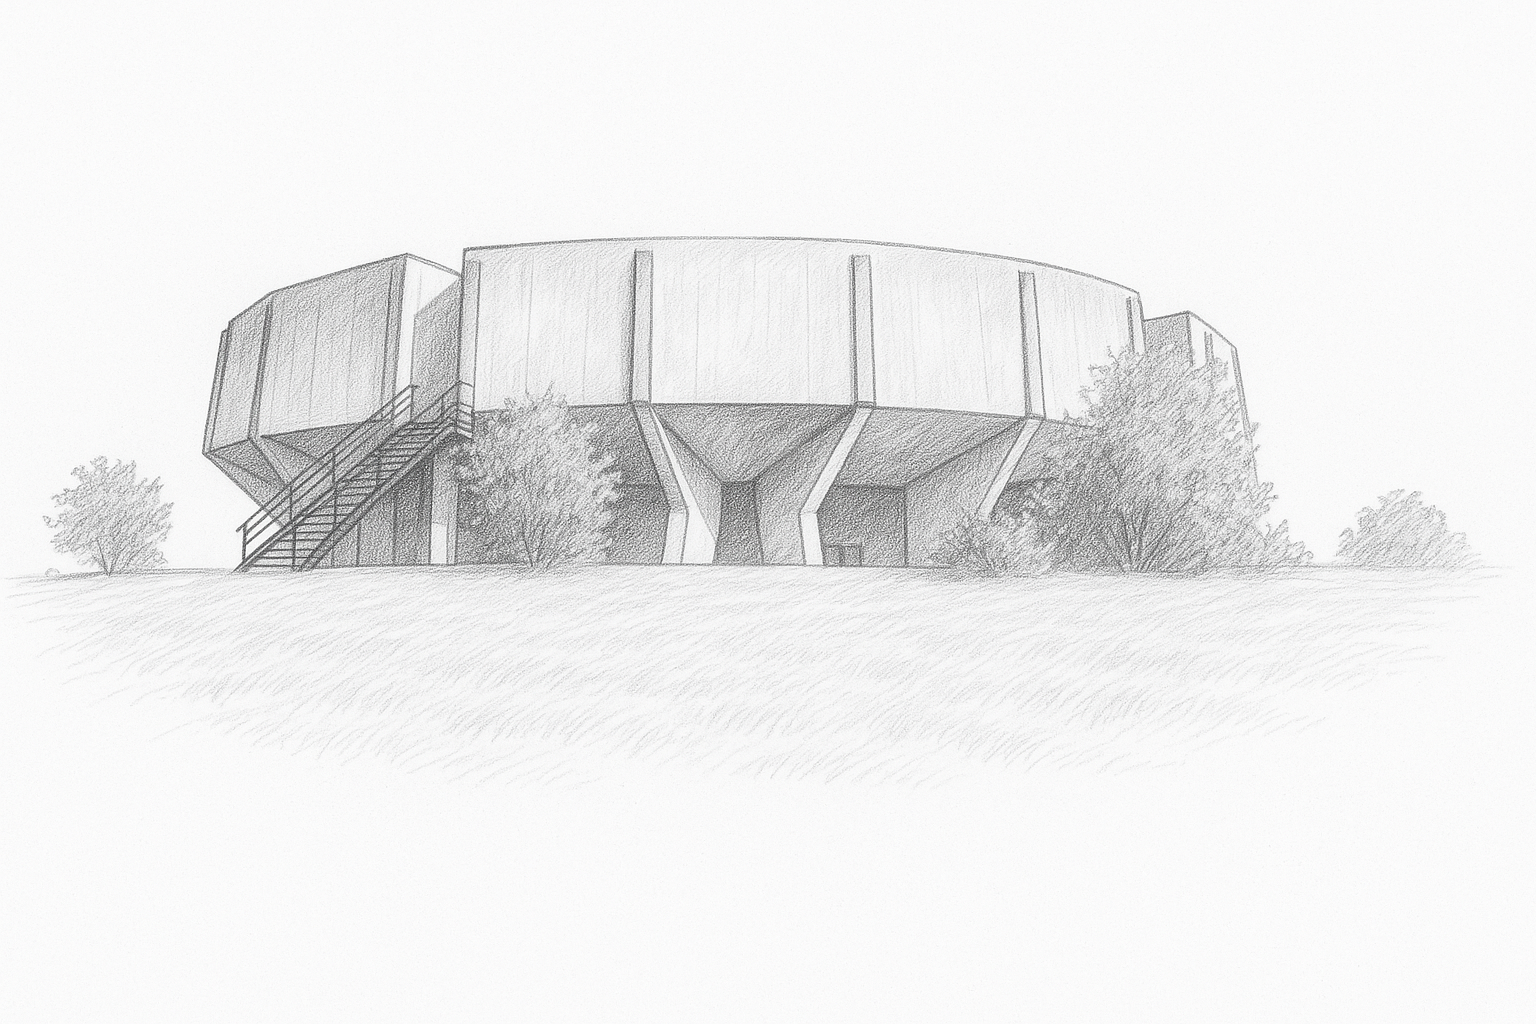
\includegraphics[
        width=\paperwidth,       % fill horizontally
        height=\paperheight,     % fill vertically
        keepaspectratio          % preserve aspect ratio
      ]{assets/back.png}    % <-- cover_background.png
    };
  \end{tikzpicture}%
}

% Configuration des chapitres avec fncychap (style Bjornstrup personnalisé)
\usepackage[Bjornstrup]{fncychap}

% Commandes de couleur personnalisées pour fncychap
\newcommand{\colortitlechap}{\color{gold}} % couleur du titre de chapitre en gold
\newcommand{\colornumberchap}{\color{gold}} % couleur du numéro de chapitre en gold
\newcommand{\colorbackchap}{\colorbox{burgundy}} % couleur de fond des règles en burgundy

\makeatletter

\renewcommand{\DOCH}{
    \settowidth{\py}{\CNoV\thechapter}
    \addtolength{\py}{-10pt}% 
    \fboxsep=0pt%
    \colorbackchap{\rule{0pt}{40pt}\parbox[b]{\textwidth}{\hfill}}%
    \kern-\py\raise20pt%
    \hbox{\colornumberchap\CNoV\thechapter}\\%
}

\renewcommand{\DOTI}[1]{%
    \nointerlineskip\raggedright%
    \fboxsep=\myhi%
    \vskip-1ex%
    \colorbackchap{\parbox[t]{\mylen}{\CTV\FmTi{\color{gold}#1}}}\par\nobreak%
    \vskip 40\p@%
}

\renewcommand{\DOTIS}[1]{%
    \fboxsep=0pt%
    \colorbackchap{\rule{0pt}{40pt}\parbox[b]{\textwidth}{\hfill}}\\%
    \nointerlineskip\raggedright%
    \fboxsep=\myhi%
    \colorbackchap{\parbox[t]{\mylen}{\CTV\FmTi{\color{gold}#1}}}\par\nobreak%
    \vskip 40\p@%
}

\makeatother

\author{DESPOULLAINS ROMAIN}

\begin{document}

% Title page with background image
\begin{titlepage}
    \BackgroundPic % Add the background image

    % === LOGOS EN HAUT ===

    \noindent

    \begin{minipage}[t]{0.45\textwidth}
        \raggedright
        
\includegraphics[width=4cm]{assets/logo-urca.png} 
    \end{minipage}%
    \hfill
    \begin{minipage}[t]{0.45\textwidth}
        \raggedleft
        
\includegraphics[width=5.3cm]{assets/logo.jpg}
    \end{minipage}    

      \vspace*{2.5cm}

    % === TITRE PRINCIPAL AVEC BARRES HARMONISÉES ===
    \centering
    {\color{gold}\rule{0.6\textwidth}{1pt}}\\[0.5cm]
    {\fontsize{22}{26}\selectfont \bfseries \color{burgundy} Rapport Projet}\\[0.5cm]
    {\color{gold}\rule{0.6\textwidth}{1pt}}\\[1.5cm]% === SOUS-TITRES DE PROJET ===
    \begin{minipage}{0.85\textwidth}
        \centering
        {\Large \textbf{Wave Function Collapse, modèle overlapping}}\\[0.3cm]
        {\large Approches Séquentielle, OpenMP et Kokkos (CPU + GPU)}\\[0.5cm]
    \end{minipage}

    \vspace*{7cm}

    % === INFORMATIONS PERSONNELLES ET ACADÉMIQUES ===
    \begin{minipage}{0.6\textwidth}
        \centering        \begin{tabular}{r l}
            \textbf{Auteur} & : \textit{M. Despoullains} \\
        \end{tabular}
    \end{minipage}

    \vspace*{2cm}    % === FILIÈRE ET ANNÉE ===

    {\footnotesize \textcolor{gray}{Université de Reims Champagne-Ardenne}}\\[0.2cm]
    {\footnotesize \textcolor{gray}{CHPS0701 : Algorithmique et Programmation Parallèle}}\\[0.2cm]
    {\footnotesize \textcolor{gray}{2025 - 2026}}

    \vspace*{1cm}
\end{titlepage}
\clearpage % Ensures that content following the title page starts on a new page

% === RÉSUMÉ EN FRANÇAIS ===
\chapter*{Résumé}
\addcontentsline{toc}{chapter}{Résumé}

Ce rapport présente l'implémentation et l'optimisation de l'algorithme \textbf{Wave Function Collapse} (WFC, Maxim Gumin, 2016) dans son modèle \textit{overlapping}. Le problème consiste à générer une grille $G$ qui « ressemble localement » à un échantillon $S$ donné, c'est-à-dire dont tout sous-bloc $N \times N$ apparaît au moins une fois dans $S$. \\

Nous développons d'abord une version séquentielle de référence basée sur trois primitives : extraction de tuiles toroïdale, compatibilité par bitsets packés sur \texttt{uint64\_t}, et propagation BFS niveau-synchrone. L'algorithme est ensuite parallélisé via \textbf{OpenMP} avec l'API \texttt{\#pragma omp task} explicite (sélection min-entropie chunked, propagation BFS multi-niveaux), puis porté sur \textbf{Kokkos} pour cibler les architectures CPU et GPU (CUDA) sans duplication de code. \\

Les benchmarks sur le supercalculateur \textbf{Romeo} (AMD EPYC 9654, 192 cœurs, 8 nœuds NUMA) atteignent un speedup peak de \textbf{8.23×} à 16 threads sur grille 256×256. Trois extensions opt-in sont livrées et étudiées : symétries D4, backtracking avec snapshot delta-encodé, et exécution de K attempts WFC indépendants en parallèle. Une démonstration sur \textbf{Unreal Engine 5} ferme le projet. \\

\textbf{Mots-clés :} Wave Function Collapse, génération procédurale, OpenMP \texttt{task}, Kokkos, GPU CUDA, déterminisme, calcul haute performance. \\

% === ABSTRACT EN ANGLAIS ===
\chapter*{Abstract}
\addcontentsline{toc}{chapter}{Abstract}

This report presents the implementation and optimization of the \textbf{Wave Function Collapse} (WFC, Maxim Gumin, 2016) algorithm in its \textit{overlapping} model. The problem is to generate a grid $G$ that locally resembles a given sample $S$: every $N \times N$ sub-block of $G$ must appear at least once in $S$. \\

We start from a serial reference using three core primitives: toroidal tile extraction, compatibility tables stored as packed \texttt{uint64\_t} bitsets, and level-synchronous BFS propagation. The algorithm is then parallelized using \textbf{OpenMP} with the explicit \texttt{\#pragma omp task} API (chunked min-entropy reduction and multi-level BFS), and ported to \textbf{Kokkos} to target both CPU and GPU (CUDA) backends without code duplication. \\

Benchmarks on the \textbf{Romeo} supercomputer (AMD EPYC 9654, 192 cores, 8 NUMA nodes) reach a peak speedup of \textbf{8.23×} at 16 threads on a 256×256 grid. Three opt-in extensions are delivered and analyzed: D4 symmetries, delta-encoded backtracking, and K independent WFC attempts running in parallel. An \textbf{Unreal Engine 5} demonstration closes the project. \\

\textbf{Keywords:} Wave Function Collapse, procedural generation, OpenMP \texttt{task}, Kokkos, CUDA GPU, determinism, high-performance computing. \\

% === TABLE DES MATIÈRES ===
\tableofcontents
\clearpage

% === LISTE DES FIGURES ===
\listoffigures
\addcontentsline{toc}{chapter}{Liste des figures}
\clearpage

% === LISTE DES TABLEAUX ===
\listoftables
\addcontentsline{toc}{chapter}{Liste des tableaux}
\clearpage

% =============================================================================
% INCLUSION DES CHAPITRES
% =============================================================================

% Chapitre 1 : Introduction
\chapter{Introduction}

\section{Sujet et stratégie}

Le \textbf{Wave Function Collapse} (WFC) en modèle \textit{overlapping} \cite{gumin2016wfc} prend un échantillon $S$ et un paramètre $N$, et produit une grille $G$ telle que tout sous-bloc $N \times N$ de $G$ apparaisse dans $S$. L'algorithme combine deux primitives : \textit{sélection min-entropie} (choisir la cellule la plus contrainte) et \textit{propagation BFS} (intersecter les contraintes des voisins). Il est intrinsèquement séquentiel sur l'arbre de décisions, mais offre du parallélisme \emph{intra-niveau} : le scan d'entropie et la propagation BFS niveau-synchrone se chunkent sur threads.

\begin{figure}[H]
\centering
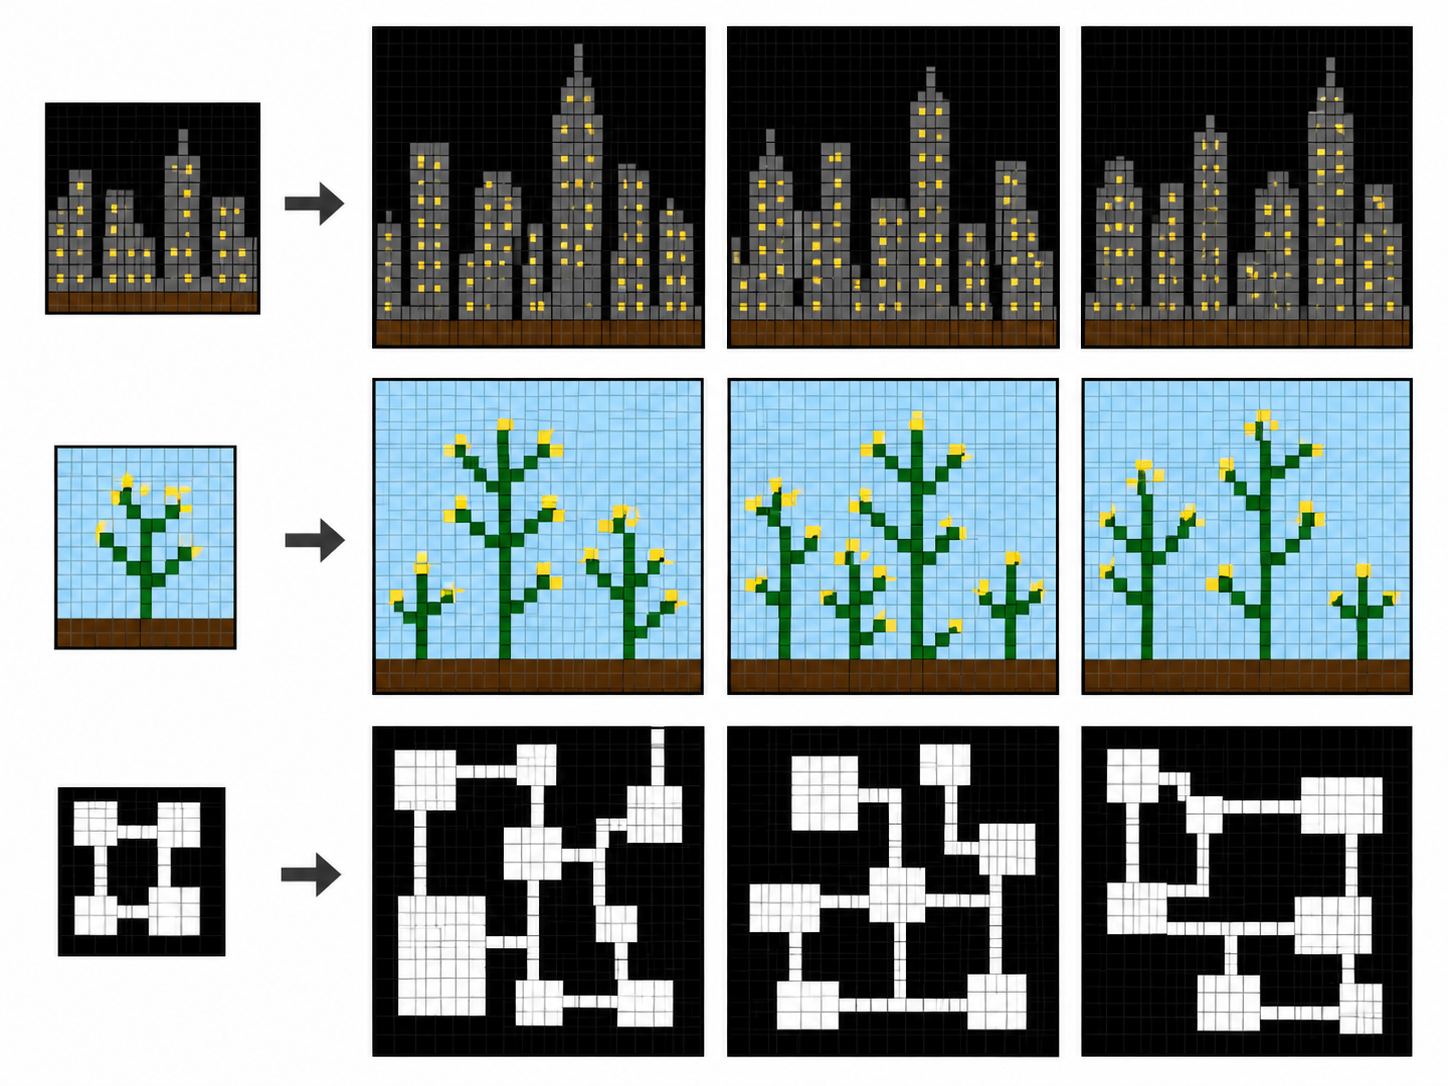
\includegraphics[width=0.85\linewidth]{results/figures/schemas/wfc_paper_outputs.png}
\caption{Sorties WFC à partir de petits échantillons : skyline urbain, plante, dungeon binaire. Chaque ligne montre l'input à gauche et trois sorties générées avec des seeds différents.}
\label{fig:wfc_paper_outputs}
\end{figure}

\subsection{Stratégie d'implémentation}

Trois cibles incrémentales :
\begin{enumerate}
    \item \textbf{Solveur série} (\texttt{wfc\_serial}) : référence algorithmique, bitsets packés sur \texttt{uint64\_t}, BFS niveau-synchrone, jitter d'entropie déterministe SplitMix64.
    \item \textbf{Backend OpenMP} (\texttt{wfc\_omp}) : API \texttt{\#pragma omp task} explicite. Sélection min-entropie chunkée + réduction ordonnée. Propagation pilotée par une seule région \texttt{parallel} (les barrières par niveau seraient catastrophiques sur 8000 niveaux BFS).
    \item \textbf{Backend Kokkos} (\texttt{wfc\_kokkos}) : même code source pour CPU OpenMP et GPU CUDA, branche compile-time \texttt{kHostOnly} pour le zero-copy CPU vs \texttt{deep\_copy} GPU.
\end{enumerate}

Tous trois produisent un output \textbf{bit-identique} pour un même seed, vérifié par hash SHA-256. Cette contrainte oriente plusieurs choix : RNG stateless, réduction en ordre de chunk fixe, atomics commutatives.

Quatre extensions opt-in : parallel-attempts, symétries D4, backtracking delta-encodé, démo Unreal Engine 5.7.

\subsection{Problèmes rencontrés}

Trois difficultés majeures pendant le développement, traitées dans les chapitres correspondants :

\begin{itemize}
    \item \textbf{Régression OMP fork/join} : ouvrir une région \texttt{parallel} par niveau BFS coûte $\sim 50$ µs $\times$ 8000 niveaux $= 400$ ms d'overhead pur, plus que le travail utile. Résolu par une seule région \texttt{parallel} ouverte avec \texttt{single} pilotant les niveaux (Section~\ref{sec:omp:propagate}).
    \item \textbf{Kokkos finalize crash} : Views cachées dans \texttt{thread\_local} désallouées \emph{après} le \texttt{finalize} de Kokkos. Résolu par \texttt{push\_finalize\_hook} (Section~\ref{sec:kokkos:cleanup}).
    \item \textbf{GPU plus lent que CPU} : sur GH200, transferts H$\leftrightarrow$D par appel à \texttt{propagate} dominent (16 GB pour 256$\times$256). Documenté comme limite structurelle, pas un bug (Section~\ref{sec:res:kokkos}).
\end{itemize}

\subsection{Analyse de performance}

220+ runs SLURM sur Romeo (EPYC 9654, 192 cœurs, 8 NUMA), avec variation systématique de :

\begin{itemize}
    \item \textbf{Taille de grille} : 32$\times$32 à 256$\times$256.
    \item \textbf{Sample (input)} : binary\_L11 (référence), terrain\_L33 (multi-valeurs riche), smooth\_N3 (cas pathologique).
    \item \textbf{Threads OpenMP} : 1, 2, 4, 8, 16, 32, 64, 192.
    \item \textbf{Backend} : serial, omp, kokkos (CPU + GPU).
\end{itemize}

Métriques calculées : speedup, efficacité parallèle, throughput, heatmap taille$\times$threads, fit Amdahl par configuration. Détails Chapitre~\ref{chap:resultats}.

\textbf{Speedup peak observé : 8.23$\times$ à 16 threads sur 256$\times$256 binary\_L11.}

\section{Organisation du rapport}

\begin{itemize}
    \item Chap.~\ref{chap:preliminaires} : préliminaires (complexité, OpenMP, Kokkos, métriques).
    \item Chap.~\ref{chap:probleme_wfc} : formalisation du problème WFC overlapping.
    \item Chap.~\ref{chap:approche} : algorithme séquentiel.
    \item Chap.~\ref{chap:implementation} : implémentation C++ (Bitset, Wave, CMake).
    \item Chap.~\ref{chap:openmp} : backend OpenMP, optims A/B.
    \item Chap.~\ref{chap:kokkos} : backend Kokkos GPU-portable.
    \item Chap.~\ref{chap:extensions} : extensions opt-in (parallel-attempts, D4, backtrack, UE5).
    \item Chap.~\ref{chap:protocole} : protocole expérimental.
    \item Chap.~\ref{chap:resultats} : résultats et analyse (speedup, scaling, Amdahl, varying input/config).
    \item Chap.~\ref{chap:limites} : limites et pistes (NUMA partitioning, batch GPU, PQ incrémentale).
    \item Chap.~\ref{chap:conclusion} : bilan.
\end{itemize}


% Chapitre 2 : Préliminaires
\chapter{Préliminaires}
\label{chap:preliminaires}

Ce chapitre introduit les concepts fondamentaux nécessaires à la compréhension des techniques employées dans ce rapport. Nous présentons les notions de complexité algorithmique, les paradigmes de programmation parallèle (OpenMP et Kokkos), ainsi que les métriques de performance utilisées pour évaluer nos implémentations.

% =============================================================================
\section{Complexité algorithmique}
\label{sec:prelim:complexite}
% =============================================================================

\subsection{Notations asymptotiques}

L'analyse de complexité permet d'évaluer le comportement d'un algorithme en fonction de la taille de l'entrée. Nous utilisons les notations asymptotiques standard :

\begin{definition}[Notation $O$ (grand O)]
Soit $f, g : \mathbb{N} \to \mathbb{R}^+$. On dit que $f(n) = O(g(n))$ s'il existe des constantes $c > 0$ et $n_0$ telles que :
\[
\forall n \geq n_0 : f(n) \leq c \cdot g(n)
\]
\end{definition}

\begin{definition}[Notation $\Theta$ (grand Theta)]
$f(n) = \Theta(g(n))$ si $f(n) = O(g(n))$ et $g(n) = O(f(n))$, c'est-à-dire si $f$ et $g$ ont le même ordre de croissance asymptotique.
\end{definition}

\subsection{Classes de complexité courantes}

\begin{table}[H]
\centering
\begin{tabular}{lll}
\toprule
\textbf{Classe} & \textbf{Nom} & \textbf{Exemple WFC} \\
\midrule
$O(1)$ & Constante & \texttt{Bitset::test(i)}, \texttt{popcount} d'un mot \\
$O(\log n)$ & Logarithmique & Allocation \texttt{vector::reserve} amortie \\
$O(n)$ & Linéaire & Scan d'une cellule de $L$ tuiles \\
$O(n^2)$ & Quadratique & Construction \texttt{OverlapRules} pour $L^2$ paires \\
$O(2^n)$ & Exponentielle & Énumération exhaustive des solutions WFC (théorique) \\
\bottomrule
\end{tabular}
\caption{Classes de complexité avec exemples tirés de l'implémentation WFC.}
\label{tab:complexity_classes}
\end{table}

\subsection{Le cas WFC}

WFC est un \textbf{problème de satisfaction de contraintes} (CSP). La résolution exhaustive serait exponentielle ($O(L^{\text{rows} \cdot \text{cols}})$ dans le pire cas). L'algorithme de Gumin contourne cela par une heuristique gloutonne : on choisit toujours la cellule d'\textbf{entropie minimale}, on collapse selon les fréquences, puis on propage les contraintes. La complexité \textit{moyenne} est polynomiale (proche du linéaire en nombre de cellules pour les samples bien comportés), mais des contradictions peuvent survenir et provoquer un retry.

% =============================================================================
\section{Programmation parallèle : concepts fondamentaux}
\label{sec:prelim:parallele}
% =============================================================================

\subsection{Motivation}

La loi de Moore, qui prédisait un doublement de la densité des transistors tous les 18 mois, a atteint ses limites physiques. Depuis le milieu des années 2000, l'augmentation des performances passe principalement par le parallélisme :
\begin{itemize}
    \item \textbf{Multicœur} : plusieurs unités de calcul sur une même puce (jusqu'à 192 cœurs sur EPYC 9654).
    \item \textbf{SIMD} : une instruction, plusieurs données (AVX-512 traite 512 bits par cycle).
    \item \textbf{GPU} : milliers de cœurs SIMT, optimisés pour le data-parallelism massif (NVIDIA GH200 = 16 896 cœurs CUDA).
    \item \textbf{Clusters} : plusieurs machines interconnectées, distribuant le travail via MPI ou frameworks task-based.
\end{itemize}

\subsection{Modèles de parallélisme}

\begin{definition}[Mémoire partagée vs distribuée]
\begin{itemize}
    \item \textbf{Mémoire partagée} : tous les threads accèdent à un espace mémoire commun. Synchronisation par locks, atomics, barrières. Modèle d'OpenMP et de Kokkos en mode multi-thread.
    \item \textbf{Mémoire distribuée} : chaque processus a sa mémoire propre, communication par messages. Modèle de MPI.
\end{itemize}
\end{definition}

WFC se prête naturellement à la mémoire partagée : la wave est un buffer plat unique, partagée par tous les threads, qui modifient des cellules différentes en parallèle (BFS niveau-synchrone). MPI ne serait pertinent que pour distribuer plusieurs solveurs sur un cluster, ce qui ne change pas la nature du calcul intra-solveur.

\subsection{OpenMP : tasks explicites}

OpenMP \cite{openmp45} est l'API standard pour le parallélisme à mémoire partagée en C++. Il offre plusieurs modèles :
\begin{itemize}
    \item \texttt{\#pragma omp parallel for} : distribution statique d'une boucle (work-sharing classique).
    \item \texttt{\#pragma omp task} : tâches dynamiques créées explicitement, exécutées par un pool de threads. Adapté aux calculs irréguliers (récursifs, BFS).
    \item \texttt{\#pragma omp atomic} : opérations atomiques sur variables partagées.
\end{itemize}

Le \textbf{sujet impose l'API \texttt{task} explicite}. Cette contrainte n'est pas arbitraire : le BFS de WFC produit des frontières de taille variable (de 1 à plusieurs centaines de cellules par niveau). Une distribution statique \texttt{parallel for} sous-utiliserait les threads sur les niveaux courts et oversubscriberait sur les niveaux longs. Les tasks dynamiques amortissent mieux cette irrégularité.

\subsection{Kokkos : portabilité CPU + GPU}

Kokkos \cite{kokkos2014} est un framework C++ développé par les laboratoires DOE (Sandia, Oak Ridge, Argonne) qui abstrait les architectures parallèles modernes. Le même code source compile vers :
\begin{itemize}
    \item OpenMP, Threads, Serial (CPU) ;
    \item CUDA (NVIDIA), HIP (AMD), SYCL (Intel) sur GPU.
\end{itemize}

Les primitives clés sont \texttt{Kokkos::View<T*>} (conteneur de tableau qui peut vivre sur \texttt{HostSpace} ou \texttt{CudaSpace}) et \texttt{Kokkos::parallel\_for} (équivalent abstrait de \texttt{omp parallel for} ou de kernel CUDA selon le backend choisi). Le coût d'utilisation : il faut suivre les conventions Kokkos (\texttt{KOKKOS\_INLINE\_FUNCTION}, pas d'allocation dynamique dans le kernel, capture par valeur des structures triviales).

% =============================================================================
\section{Métriques de performance}
\label{sec:prelim:metriques}
% =============================================================================

\subsection{Speedup}

\begin{definition}[Speedup]
Le speedup d'une exécution parallèle à $p$ threads est défini par :
\[
S(p) = \frac{T(1)}{T(p)}
\]
où $T(1)$ est le temps série et $T(p)$ le temps à $p$ threads.
\end{definition}

Idéalement, $S(p) = p$ (scaling linéaire). En pratique, $S(p) < p$ à cause des coûts de synchronisation, de la fraction séquentielle, et du contention mémoire.

\subsection{Efficacité parallèle}

\begin{definition}[Efficacité parallèle]
\[
E(p) = \frac{S(p)}{p} = \frac{T(1)}{p \cdot T(p)}
\]
\end{definition}

$E(p) \in [0, 1]$. Une efficacité de 0.5 signifie que la moitié des threads sont effectivement productifs, l'autre moitié est en attente ou en redondance.

\subsection{Loi d'Amdahl}

\begin{theorem}[Loi d'Amdahl \cite{amdahl1967}]
Si une fraction $f$ d'un programme est parallélisable et $(1 - f)$ est intrinsèquement séquentielle, le speedup maximum atteignable avec $p$ threads est :
\[
S(p) = \frac{1}{(1 - f) + \frac{f}{p}}
\]
Le ceiling théorique quand $p \to \infty$ vaut :
\[
S_{\max} = \frac{1}{1 - f}
\]
\end{theorem}

\begin{important}{Conséquence pratique pour WFC}
Un fit Amdahl sur les mesures Romeo donne $f \approx 0.944$ pour binary\_L11 256×256. Le ceiling théorique est donc $S_{\max} \approx 17.8$, mais le peak observé n'atteint que 8.23× à 16 threads. La différence (54\%) provient des coûts non-Amdahl : NUMA, contention atomique, fork/join répété, dont le modèle ne tient pas compte.
\end{important}

\subsection{Strong scaling vs weak scaling}

\begin{definition}[Strong scaling]
Mesure de $S(p)$ à \textbf{taille de problème fixe} et nombre de threads $p$ croissant. Question posée : « combien de threads pour résoudre le problème plus vite ? »
\end{definition}

\begin{definition}[Weak scaling]
Mesure de $T(p)$ à \textbf{taille de problème par thread fixe} (le problème grandit proportionnellement à $p$). Question posée : « combien de fois plus gros peut-on aller avec plus de threads ? »
\end{definition}

Les benchmarks de ce rapport sont \textit{strong scaling} : on mesure $T(p)$ pour des grilles fixées (32, 64, 128, 256, 512) à threads croissants.

% =============================================================================
\section{Architectures cibles}
\label{sec:prelim:archi}
% =============================================================================

\subsection{Hiérarchie mémoire}

Les performances HPC dépendent fortement de la hiérarchie mémoire. Sur EPYC 9654 :
\begin{itemize}
    \item \textbf{Registres} : ~1 ns d'accès, quelques centaines de bits.
    \item \textbf{L1} : 32 KB par cœur, latence ~4 cycles.
    \item \textbf{L2} : 1 MB par cœur, latence ~12 cycles.
    \item \textbf{L3} : 32 MB par CCX (chaque CCX groupe 8 cœurs), latence ~50 cycles.
    \item \textbf{DRAM locale au socket} : ~80 ns.
    \item \textbf{DRAM cross-socket} : ~140 ns (1.7× plus cher).
\end{itemize}

Pour WFC, la \textbf{wave} occupe 16 KB pour 64×64 binaire (tient en L2), 65 KB pour 128×128 (déborde L1), 524 KB pour 256×256 (déborde L2 par cœur). C'est ce qui explique en partie pourquoi le speedup est meilleur sur 256×256 que sur 128×128 : à 256, on passe plus de temps en attente mémoire, ce que le parallélisme aide à amortir.

\subsection{NUMA}

Sur EPYC 9654, les 192 cœurs sont organisés en \textbf{8 nœuds NUMA} (3 CCDs par nœud, 8 cœurs par CCD). Un accès mémoire \textit{cross-NUMA} coûte ~3× plus cher qu'un accès local.

L'optimisation classique est le \textit{first-touch} : lors de l'allocation d'un tableau partagé, le thread qui le \textit{touche en premier} est celui qui reçoit la page physique sur son nœud NUMA. Pour WFC, le constructeur de \texttt{Wave} parallélise l'initialisation par \texttt{\#pragma omp parallel for}, ce qui mappe correctement les pages aux nœuds NUMA des threads consommateurs.

\subsection{GPU NVIDIA GH200}

La partition \texttt{armgpu} de Romeo dispose de \textbf{NVIDIA GH200 Grace Hopper}, qui combine :
\begin{itemize}
    \item un CPU ARM Neoverse-V2 (72 cœurs) ;
    \item un GPU H100 (132 SMs, 16 896 cœurs CUDA) ;
    \item 97 GB de mémoire HBM3 sur le GPU.
\end{itemize}

L'ensemble communique via \textbf{NVLink-C2C}, avec une bande passante ~4× supérieure au PCIe 5. C'est l'architecture cible que nous utilisons pour le port Kokkos+CUDA.


% Chapitre 3 : Problème WFC (modèle overlapping)
\chapter{Le problème : Wave Function Collapse}
\label{chap:probleme_wfc}

\section{Origine et intuition}

\subsection{De la mécanique quantique à la génération procédurale}

Le \textbf{Wave Function Collapse} (WFC) tire son nom d'une analogie avec la mécanique quantique. Dans une expérience de pensée comme le chat de Schrödinger, le système reste en \textit{superposition} de plusieurs états (vivant et mort) jusqu'à ce qu'une mesure le fasse \textit{collapser} dans un état unique. WFC applique cette image à la génération procédurale : chaque cellule de la grille de sortie commence en superposition de toutes les valeurs possibles, puis se collapse progressivement par propagation de contraintes locales \cite{heaton2018wfc}.

L'algorithme a été publié par Maxim Gumin en 2016 \cite{gumin2016wfc} sous licence MIT et a connu un succès important : il est utilisé dans des jeux commerciaux comme \textit{Townscaper}, \textit{Caves of Qud}, \textit{Bad North}, et dans de nombreux outils de level design.

\subsection{Le problème en termes formels}

Soit $S$ une grille rectangulaire de taille $r_S \times c_S$ à valeurs dans un alphabet $\Sigma$ (typiquement $\{0, 1\}$ pour le cas binaire, ou $\{0, 1, \ldots, K-1\}$ pour le cas multi-valeurs). Soit $N \in \mathbb{N}^*$ la taille de tuile, et $G$ une grille de taille $r_G \times c_G$ à valeurs dans $\Sigma$ que l'on cherche à construire.

\begin{definition}[Sous-bloc $N \times N$]
Un \textbf{sous-bloc} de taille $N \times N$ d'une grille $H$ à la position $(r, c)$ est l'ensemble des valeurs $H[(r+i) \bmod r_H][(c+j) \bmod c_H]$ pour $0 \leq i, j < N$, avec wrap-around toroïdal.
\end{definition}

\begin{definition}[Tuile valide]
Une tuile $T$ est \textbf{valide} pour $S$ si elle apparaît au moins une fois comme sous-bloc $N \times N$ de $S$.
\end{definition}

\begin{definition}[Solution WFC]
Une grille $G$ est une \textbf{solution WFC} pour $(S, N)$ si tout sous-bloc $N \times N$ de $G$ est une tuile valide pour $S$.
\end{definition}

\subsection{Exemple littéral du sujet}

Le \texttt{README.pdf} du sujet propose l'échantillon binaire suivant ($r_S = c_S = 5$) :

\begin{verbatim}
1 0 1 1 1
1 0 1 1 1
0 0 1 1 1
0 1 1 1 1
0 0 0 0 0
\end{verbatim}

Pour $N = 2$, l'extraction non-toroïdale identifie 8 tuiles distinctes ; l'extraction \textbf{toroïdale} (notre choix de design, voir Chapitre~\ref{chap:approche}) en identifie 11. Le solveur produit ensuite une grille $G$ de taille libre (par exemple $64 \times 64$) qui ne contient localement que ces tuiles.

\begin{figure}[H]
\centering
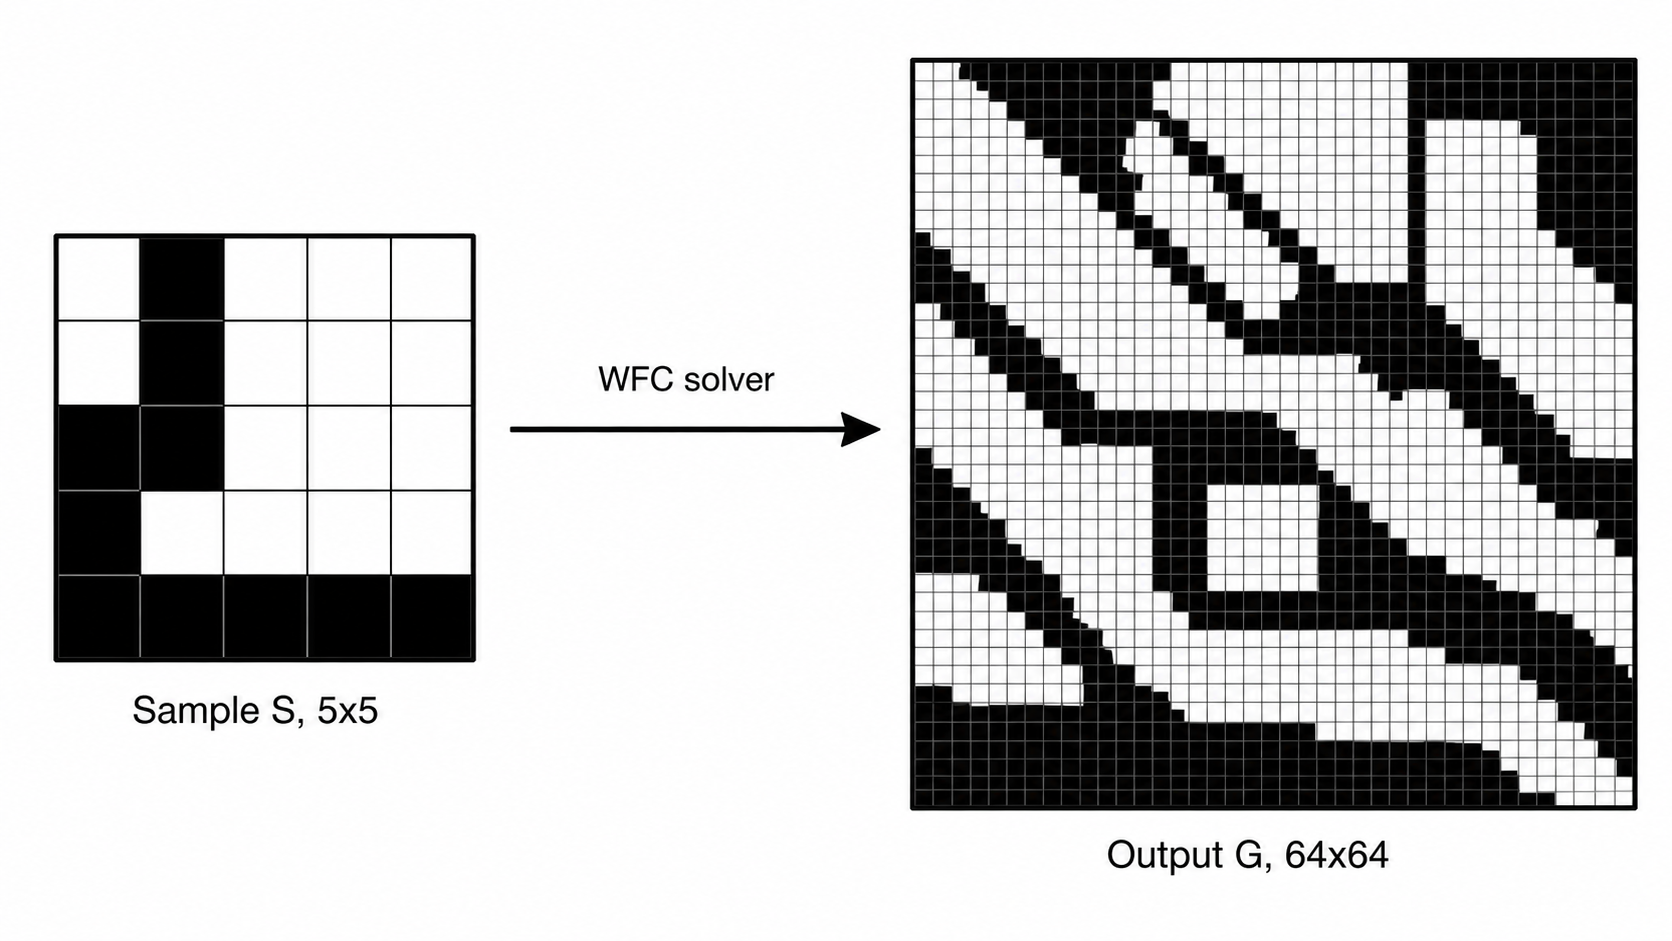
\includegraphics[width=0.85\linewidth]{results/figures/schemas/sample_to_output.png}
\caption{Pipeline WFC en une figure : à partir d'un petit échantillon $S$ (5×5), le solveur reproduit les motifs locaux dans une grille $G$ de taille libre (64×64).}
\label{fig:sample_to_output}
\end{figure}

\section{Le modèle overlapping}

WFC se décline en plusieurs variantes. Le \textbf{Simple Tiled Model} utilise une palette finie de tuiles avec contraintes d'adjacence données explicitement (utile pour les sprites de jeux). Le \textbf{Simple Tiled Model symétrique} ajoute la gestion des rotations / réflexions des tuiles. Le \textbf{modèle overlapping} (notre choix, imposé par le sujet) extrait les contraintes par recouvrement entre sous-blocs $N \times N$ de l'échantillon.

\subsection{Définition formelle des contraintes overlapping}

\begin{definition}[Compatibilité overlapping]
Deux tuiles $t_1$ et $t_2$ de taille $N \times N$ sont \textbf{compatibles} à un offset $(dx, dy)$ avec $|dx|, |dy| \leq N - 1$ si leurs valeurs coïncident sur la zone de recouvrement :
\[
\forall (x, y) \in [\max(0, -dx), \min(N-1, N-1-dx)] \times [\max(0, -dy), \min(N-1, N-1-dy)] :
\]
\[
t_1[y + dy][x + dx] = t_2[y][x]
\]
\end{definition}

Pour deux tuiles $2 \times 2$, il y a $(2N - 1)^2 = 9$ offsets pertinents (incluant $(0, 0)$ qui correspond à l'identité $t_1 = t_2$).

\subsection{Symétrie des règles}

\begin{theorem}[Symétrie des règles d'adjacence]
Pour toute paire de tuiles $(t_1, t_2)$ et tout offset $(dx, dy)$ :
\[
t_2 \in \text{allowed}(t_1, dx, dy) \iff t_1 \in \text{allowed}(t_2, -dx, -dy)
\]
\end{theorem}

Cette propriété est utilisée par notre suite de tests (\texttt{test\_overlap}) comme \textit{invariant} de validation, vérifiant en particulier que la convention d'offset est implémentée correctement (un bug subtil que nous avons détecté pendant le développement par cette voie).

% =============================================================================
\section{Applications}
\label{sec:wfc:applications}
% =============================================================================

\subsection{Jeux vidéo et level design}

WFC est massivement utilisé pour la génération procédurale de niveaux :
\begin{itemize}
    \item \textbf{Townscaper} (Oskar Stålberg, 2020) : les bâtiments sont composés en temps réel par WFC à partir d'un set de tuiles 3D.
    \item \textbf{Caves of Qud} : génération de cavernes et donjons.
    \item \textbf{Bad North} : génération des îles tactiques.
\end{itemize}

Notre démonstration UE5 (\texttt{wfc\_dungeon}, voir Chapitre~\ref{chap:extensions}) reproduit ce paradigme : génération d'un dungeon mono-étage exporté en JSON, consommé par un plugin Unreal qui spawne les meshes 3D et des actors gameplay (PlayerStart, NPC spawners, pickups) dans un \texttt{ADungeonGenerator}.

\subsection{Synthèse de textures}

WFC peut être appliqué à la synthèse de textures de grande taille à partir d'un échantillon de référence \cite{efros1999texture}. Le résultat est moins fidèle que les méthodes basées sur les réseaux de neurones (StyleGAN, etc.) mais il est entièrement déterministe et explicable.

\subsection{Inpainting et complétion}

Une extension de WFC permet le \textit{inpainting} : étant donnée une grille partiellement remplie, compléter les cellules manquantes en respectant les contraintes locales. Cette extension n'est pas implémentée dans notre projet, mais l'architecture s'y prête (il suffirait de pré-collapser certaines cellules avant de lancer le solveur).

\subsection{Création artistique}

L'algorithme est utilisé en art génératif (motifs cellulaires, mosaïques, calligraphie procédurale). Sa simplicité conceptuelle le rend accessible aux artistes non-programmeurs via des outils comme \textit{WFC Studio} ou des plugins Blender.

% =============================================================================
\section{Difficultés calculatoires}
\label{sec:wfc:difficultes}
% =============================================================================

\subsection{Espace de recherche exponentiel}

Pour une grille $r \times c$ avec $L$ tuiles candidates par cellule, l'espace de recherche brut est $L^{r \cdot c}$. Pour $L = 11$, $r = c = 128$, cela représente $11^{16384} \approx 10^{17040}$ configurations possibles. L'énumération exhaustive est exclue.

\subsection{Heuristique gloutonne}

L'algorithme de Gumin contourne cette explosion par une heuristique gloutonne en deux phases :
\begin{enumerate}
    \item \textbf{Sélection min-entropie} : choisir la cellule la plus contrainte (peu de candidats restants) avant les autres.
    \item \textbf{Propagation BFS} : après chaque collapse, propager les contraintes en intersectant les ensembles de candidats des voisins.
\end{enumerate}

L'heuristique réduit drastiquement l'espace exploré mais ne garantit pas la convergence : une succession de mauvais choix peut conduire à un \textbf{contradiction} (cellule à 0 candidats), nécessitant un retry.

\subsection{Contradictions et stratégies de récupération}

Trois stratégies sont possibles face à une contradiction :
\begin{enumerate}
    \item \textbf{Restart} (notre défaut) : abandonner la tentative, recommencer avec un nouveau seed dérivé. Simple, peu invasif, suffisant en pratique sur les samples bien comportés.
    \item \textbf{Backtracking} (notre option \texttt{--backtrack}) : revenir au dernier point de décision, essayer un autre choix. Plus puissant sur samples très contraints, plus complexe (snapshot/restore).
    \item \textbf{Soft constraints} : tolérer certaines violations à coût pondéré (non implémenté).
\end{enumerate}

\subsection{Complexité de la sélection min-entropie}

Le profilage de notre solveur série (Chapitre~\ref{chap:resultats}) révèle un résultat contre-intuitif : la \textbf{sélection min-entropie domine le temps total ($\sim 85\%$)}, pas la propagation ($\sim 12\%$). À chaque collapse, l'algorithme re-scanne toutes les $r \cdot c$ cellules pour trouver celle d'entropie minimale. Ce coût en $O(r \cdot c \cdot L)$ par collapse, multiplié par les $\sim r \cdot c$ collapses au total, donne $O((r \cdot c)^2 \cdot L)$ opérations dans la version naïve.

C'est cette étape qui justifie l'effort principal de parallélisation (\texttt{parallel\_min\_entropy} via tasks OMP).


% Chapitre 4 : Approche algorithmique séquentielle
\chapter{Approche algorithmique séquentielle}
\label{chap:approche}

\epigraph{\textit{``The art of programming is the art of organizing complexity.''}}{--- Edsger W. Dijkstra}

Ce chapitre détaille l'algorithme WFC tel que nous l'avons implémenté en série. Il sert de référence pour les chapitres parallèles : les versions OpenMP et Kokkos partagent exactement la même logique, seuls les schémas d'orchestration diffèrent.

\section{Les six étapes de WFC}

L'algorithme WFC se résume en six étapes, alignées sur la formulation de Gumin \cite{gumin2016wfc} et la présentation pédagogique de Heaton \cite{heaton2018wfc}.

\begin{algorithm}[H]
\caption{Wave Function Collapse séquentiel}
\begin{algorithmic}[1]
\Require Échantillon $S$, taille de tuile $N$, dimensions sortie $(r, c)$, seed
\Ensure Grille $G$ ou échec
\State $T, \text{freq} \gets \textsc{ExtraireTuiles}(S, N)$
\State $R \gets \textsc{ConstruireRègles}(T, N)$
\State $W \gets \textsc{InitWave}(r, c, |T|)$ \Comment{toutes tuiles candidates partout}
\State $\text{rng} \gets \textsc{Mt19937}(\text{seed})$
\Loop
    \State $\text{cell} \gets \arg\min_c \textsc{Entropy}(W[c]) + \textsc{Jitter}(c, \text{seed})$
    \If{$\text{cell} = -1$}
        \State \Return \textsc{BuildOutput}($W$, $T$) \Comment{succès}
    \EndIf
    \State $t \gets \textsc{WeightedPick}(W[\text{cell}], \text{freq}, \text{rng})$
    \State $W[\text{cell}] \gets \{t\}$ \Comment{collapse}
    \If{$\neg \textsc{Propagate}(W, R, \text{cell})$}
        \State \Return $\bot$ \Comment{contradiction}
    \EndIf
\EndLoop
\end{algorithmic}
\end{algorithm}

\subsection{Étape 1 : Extraction des tuiles}

\begin{definition}[Extraction toroïdale]
Pour chaque position $(r_0, c_0) \in [0, r_S) \times [0, c_S)$ de l'échantillon, on lit $N \times N$ valeurs avec wrap-around :
\[
\text{tile}[i][j] = S[(r_0 + i) \bmod r_S][(c_0 + j) \bmod c_S]
\]
\end{definition}

L'algorithme accumule les tuiles dans une \texttt{unordered\_map<Tile, int>} pour dédupliquer en $O(1)$ amorti par hash FNV-1a. Pour chaque tuile rencontrée, sa fréquence est incrémentée. Le résultat : un vecteur $T$ des tuiles uniques et un vecteur \texttt{freq} parallèle.

\paragraph{Choix toroïdal vs non-toroïdal.} Le sujet ne précise pas la convention. Nous choisissons \textbf{toroïdal} pour deux raisons :
\begin{itemize}
    \item Chaque pixel apparaît exactement dans $N \times N$ tuiles, distribution uniforme.
    \item Le nombre total de tuiles extraites vaut $r_S \times c_S$ (et non $(r_S - N + 1) \times (c_S - N + 1)$), ce qui évite les biais de bord.
\end{itemize}

C'est aussi le choix de l'implémentation référence de Gumin. Pour l'exemple du sujet ($5 \times 5$ binaire avec $N = 2$), l'extraction toroïdale identifie 11 tuiles uniques (vs 8 en non-toroïdal). Tests \texttt{test\_tileset} valident ces 11 tuiles bit-à-bit.

\subsection{Étape 2 : Pré-calcul des règles d'adjacence}

Pour chaque paire de tuiles $(t_1, t_2)$ et chaque offset $(dx, dy) \in [-(N-1), N-1]^2$, on calcule un booléen : « $t_2$ est-elle compatible avec $t_1$ au décalage $(dx, dy)$ ? ». Le résultat est stocké comme \textbf{bitset} indexé par identifiant de tuile.

\begin{figure}[H]
\centering
\schemaImage{Compatibilite overlap entre tuiles 2x2}
\caption{Convention d'overlap : $t_2$ placée à $(dx, dy)$ de $t_1$, les valeurs doivent coïncider sur la zone de recouvrement.}
\label{fig:overlap_compatibility}
\end{figure}

Le stockage est plat : un \texttt{vector<Bitset>} de taille $L \cdot (2N-1)^2$, indexé par
\[
\text{rule\_idx}(t, dx, dy) = t \cdot (2N-1)^2 + (dx + N - 1) \cdot (2N-1) + (dy + N - 1)
\]

\paragraph{Coût.} $L^2 \times (2N-1)^2$ paires à tester, chaque test en $O(N^2)$. Pour le sample du sujet ($L = 11$, $N = 2$) : $\sim 5000$ comparaisons, exécutées en quelques µs. Pour $L = 73$, $N = 3$ : $\sim 500\,000$ comparaisons, encore quelques ms. Cette construction est parallélisée en OpenMP via \texttt{\#pragma omp parallel for} sur la boucle externe (gain $\sim 2\times$ sur 8 cores).

\subsection{Étape 3 : Initialisation de la Wave}

Chaque cellule $(r, c)$ de la grille de sortie reçoit le bitset \textbf{plein} (toutes les $L$ tuiles candidates). Le constructeur de \texttt{Wave} fait un \textit{first-touch parallèle} (\texttt{\#pragma omp parallel for} sur l'init) pour mapper les pages physiques sur le nœud NUMA des threads consommateurs.

\subsection{Étape 4 : Sélection min-entropie}

\begin{definition}[Entropie de Shannon pondérée]
Pour une cellule $c$ dont l'ensemble de candidats restants est $W[c]$, l'entropie est :
\[
H(c) = \log\left(\sum_{t \in W[c]} f_t\right) - \frac{\sum_{t \in W[c]} f_t \log f_t}{\sum_{t \in W[c]} f_t}
\]
où $f_t$ est la fréquence de la tuile $t$ dans $S$.
\end{definition}

L'algorithme choisit la cellule de moindre entropie (cellule la plus contrainte). Pour départager les ex-aequo (très fréquents en début de résolution quand toutes les cellules ont la même entropie), on ajoute un \textbf{bruit déterministe} :
\[
H'(c) = H(c) + \text{jitter}(c, \text{seed})
\]
où \texttt{jitter} est un hash SplitMix64 de $(c, \text{seed})$ produisant une valeur dans $[0, 10^{-6})$. Ce bruit est \textbf{stateless} : il ne consomme pas l'état du RNG, ce qui garantit le déterminisme à travers les backends parallèles (voir Chapitre~\ref{chap:openmp}).

\subsection{Étape 5 : Tirage pondéré et collapse}

Une fois la cellule choisie, on tire une tuile selon les fréquences :
\begin{enumerate}
    \item Calculer la somme $S = \sum_{t \in W[\text{cell}]} f_t$
    \item Tirer $u \sim \mathcal{U}(0, S)$
    \item Parcourir les candidats par ordre croissant de $t$, accumuler la CDF, retourner le premier $t$ tel que $\text{CDF}(t) \geq u$.
\end{enumerate}

\texttt{wave[cell].set\_only(t)} réduit le bitset à un seul bit (force la collapse).

\subsection{Étape 6 : Propagation BFS}

\begin{algorithm}[H]
\caption{Propagation BFS niveau-synchrone}
\begin{algorithmic}[1]
\Require Wave $W$, règles $R$, cellule de départ $c_0$
\Ensure $\bot$ si contradiction, $\top$ sinon
\State $Q \gets \{c_0\}$
\While{$Q \neq \emptyset$}
    \State $c \gets Q.\textsc{Pop}()$
    \For{chaque offset $(dx, dy) \in [-(N-1), N-1]^2 \setminus \{(0,0)\}$}
        \State $nc \gets \textsc{Voisin}(c, dx, dy)$
        \State $A \gets \bigcup_{t \in W[c]} R(t, dx, dy)$ \Comment{union des compatibilités}
        \State $\text{changed} \gets W[nc] \gets W[nc] \cap A$ \Comment{intersection bitwise}
        \If{$\text{changed}$}
            \If{$W[nc] = \emptyset$}
                \State \Return $\bot$ \Comment{contradiction}
            \EndIf
            \State $Q.\textsc{Push}(nc)$
        \EndIf
    \EndFor
\EndWhile
\State \Return $\top$
\end{algorithmic}
\end{algorithm}

\paragraph{Variante \texttt{for\_each\_set} optimisée.} L'union $A$ se calcule en énumérant les bits actifs de $W[c]$ via \texttt{\_\_builtin\_ctzll} (count trailing zeros). Pour chaque bit actif, on \texttt{or\_with} la règle correspondante. Beaucoup plus rapide que tester chaque bit en $O(L)$.

% =============================================================================
\section{Stratégies de récupération sur contradiction}
\label{sec:approche:retry}
% =============================================================================

\subsection{Restart-on-contradiction (défaut)}

Quand \texttt{propagate} retourne $\bot$, l'algorithme retourne \texttt{false} pour le \texttt{run\_attempt} courant. La boucle \texttt{solve()} retente avec un nouveau seed dérivé :
\[
\text{seed}_k = \text{seed}_{\text{base}} + k \cdot \phi
\]
où $\phi = \texttt{0x9E3779B97F4A7C15}$ est l'inverse du nombre d'or 64 bits (Knuth). Jusqu'à \texttt{max\_attempts} essais.

\paragraph{Pourquoi ce choix ?} Trois raisons :
\begin{itemize}
    \item Backtracking propre = sauvegarder/restaurer l'état complet de la wave, potentiellement profond, avec impact mémoire imprédictible.
    \item En pratique, sur les samples fournis, 1-2 attempts suffisent.
    \item Pédagogiquement plus simple et lisible.
\end{itemize}

\subsection{Backtracking (option \texttt{--backtrack})}

L'extension \texttt{--backtrack} (Chapitre~\ref{chap:extensions}) implémente l'alternative : sur contradiction, dépiler le dernier point de décision et essayer le candidat suivant. Le snapshot delta-encodé minimise la mémoire à $\sim 50$ cellules par frame plutôt que la wave complète.

% =============================================================================
\section{Reconstruction de la sortie}
\label{sec:approche:output}
% =============================================================================

Une fois la wave complètement collapsée (chaque cellule à 1 candidat), on reconstruit la grille $G$ :

\begin{definition}[Reconstruction]
Pour chaque cellule $(r, c)$ de la wave, on lit l'unique tuile $t = W[r][c]$ encore active. La valeur de pixel $G[r][c]$ est la valeur du \textbf{coin haut-gauche} de $t$ :
\[
G[r][c] = T[t][0][0]
\]
\end{definition}

Cette convention est nécessaire car dans le modèle overlapping, plusieurs tuiles couvrent chaque pixel. On choisit conventionnellement celui dont le coin haut-gauche est sur $(r, c)$. Vérifié par \texttt{test\_solver::output\_uses\_only\_input\_tiles}.

% =============================================================================
\section{Complexité et profilage}
\label{sec:approche:complexite}
% =============================================================================

\begin{table}[H]
\centering
\begin{tabular}{lll}
\toprule
\textbf{Étape} & \textbf{Complexité} & \textbf{Pour 128×128, $L = 11$} \\
\midrule
Extraction tuiles & $O(r_S \cdot c_S \cdot N^2)$ & $\sim 100$ µs (une fois) \\
Règles d'adjacence & $O(L^2 \cdot (2N-1)^2 \cdot N^2)$ & $\sim 50$ µs (une fois) \\
\textbf{Min-entropie} & $O(r \cdot c \cdot L)$ \textbf{par collapse} & $\sim 30$ µs \textbf{par collapse} \\
Propagation BFS & $O(r \cdot c \cdot (2N-1)^2 \cdot L)$ amorti par collapse & $\sim 150$ µs par collapse \\
Tirage RNG & $O(L)$ par collapse & $\sim 1$ µs par collapse \\
\midrule
\textbf{Total} (8000 collapses) & dominé par min-entropie + BFS & $\sim 3-4$ s en série \\
\bottomrule
\end{tabular}
\caption{Décomposition de complexité du WFC séquentiel sur grille 128×128 binaire ($L = 11$).}
\label{tab:wfc_complexity}
\end{table}

\begin{important}{Résultat contre-intuitif}
La sélection min-entropie (re-scan de la wave entière à chaque collapse) domine $\sim 85\%$ du temps total. La propagation BFS, malgré sa complexité visible plus grande, ne représente que $\sim 12\%$.

C'est ce qui justifie l'effort de parallélisation principal sur \texttt{parallel\_min\_entropy}, et non sur \texttt{propagate\_tasks} (Chapitre~\ref{chap:openmp}).
\end{important}

\section{Garanties d'invariants}

Notre suite de tests vérifie systématiquement plusieurs invariants algorithmiques (Tableau~\ref{tab:invariants}).

\begin{table}[H]
\centering
\begin{tabularx}{\textwidth}{lX}
\toprule
\textbf{Invariant} & \textbf{Vérifié par} \\
\midrule
Sortie utilise uniquement des tuiles présentes dans l'échantillon & \texttt{test\_solver::output\_uses\_only\_input\_tiles} \\
\midrule
Symétrie des règles : $t_2 \in \text{allow}(t_1, d) \iff t_1 \in \text{allow}(t_2, -d)$ & \texttt{test\_overlap} \\
\midrule
Identité au décalage $(0, 0)$ : $\text{allow}(t, 0, 0) = \{t\}$ & \texttt{test\_overlap} \\
\midrule
Total des fréquences = $r_S \cdot c_S$ (toroïdal) & \texttt{test\_tileset} \\
\midrule
Déterminisme : même seed → même output (bit-à-bit) & \texttt{test\_solver}, \texttt{test\_solver\_omp}, \texttt{test\_solver\_kokkos} \\
\midrule
Bit-identité serial = OMP = Kokkos pour un même seed et $\{1, 2, 4, 8\}$ threads & \texttt{test\_solver\_omp}, \texttt{test\_solver\_kokkos} \\
\midrule
Reseed produit une sortie différente (haute probabilité) & \texttt{test\_solver\_omp}, \texttt{test\_solver\_kokkos} \\
\bottomrule
\end{tabularx}
\caption{Invariants algorithmiques vérifiés par la suite de tests.}
\label{tab:invariants}
\end{table}


% Chapitre 5 : Implémentation C++ et ingénierie logicielle
\chapter{Implémentation C++ et ingénierie logicielle}
\label{chap:implementation}

\epigraph{\textit{``Any fool can write code that a computer can understand. Good programmers write code that humans can understand.''}}{--- Martin Fowler}

\section{Organisation du dépôt}

Le projet est organisé selon une architecture modulaire séparant clairement les interfaces, les implémentations, et les points d'entrée.

\subsection{Structure des répertoires}

\begin{lstlisting}[language=bash, caption={Arborescence du projet WFC}]
Projet801/
├── include/wfc/         # Headers publics
│   ├── Grid.hpp           # Domaine 2D
│   ├── Tile.hpp           # Sous-bloc N×N + helpers symétries
│   ├── Bitset.hpp         # Bitset packé sur uint64_t
│   ├── TileSet.hpp        # Catalogue de tuiles + fréquences
│   ├── OverlapRules.hpp   # Compatibilités tuile×offset
│   ├── Wave.hpp           # Superposition par cellule
│   ├── WFCSolver.hpp      # Interface solver + SolverOptions/Stats
│   ├── GridIO.hpp         # I/O txt, PPM, PNG
│   ├── solvers/           # Backends spécialisés
│   │   ├── WFCSolverSerial.hpp
│   │   ├── WFCSolverOMP.hpp
│   │   └── WFCSolverKokkos.hpp
│   └── internal/          # Helpers et base class
│       ├── WFCSolverBase.hpp
│       └── SolverCommon.hpp
├── src/                 # Implémentations correspondantes
├── apps/                # Points d'entrée
│   ├── wfc_serial.cpp
│   ├── wfc_omp.cpp
│   ├── wfc_kokkos.cpp
│   ├── benchmark.cpp
│   └── wfc_dungeon.cpp    # Démo UE5 (opt-in BUILD_DUNGEON)
├── tests/               # Suite de tests unitaires (15 suites)
├── samples/             # Grilles d'entrée
├── scripts/             # SLURM, plot, analyze, render
├── results/             # CSV de benchmarks
├── docs/                # Documentation projet (ARCHITECTURE, ALGORITHM, etc.)
├── ue5_plugin/          # Plugin Unreal Engine 5.7
└── third_party/         # stb_image_write.h
\end{lstlisting}

\subsection{Modules et responsabilités}

Le tableau~\ref{tab:modules} détaille la responsabilité de chaque module.

\begin{table}[H]
\centering
\begin{tabularx}{\textwidth}{lX}
\toprule
\textbf{Module} & \textbf{Responsabilité} \\
\midrule
\texttt{Grid.hpp} & Domaine 2D row-major en \texttt{uint8\_t}, accès toroïdal via \texttt{at\_torus(r, c)} \\
\midrule
\texttt{Tile.hpp} & Pattern $N \times N$ POD-like avec hash FNV-1a et helpers de symétrie (\texttt{rotated\_90}, \texttt{reflected\_horizontal}) \\
\midrule
\texttt{Bitset.hpp} & Trois classes : \texttt{Bitset} propriétaire, \texttt{BitsetView} mutable, \texttt{ConstBitsetView} lecture-seule. Opérations 64-bit packées. \\
\midrule
\texttt{TileSet.hpp/cpp} & Extraction toroïdale $N \times N$, déduplication, expansion D4 optionnelle \\
\midrule
\texttt{OverlapRules.hpp/cpp} & Construction parallèle (OMP) des règles de compatibilité \\
\midrule
\texttt{Wave.hpp} & Buffer plat de bitsets, NUMA first-touch, accès toroïdal pour BFS \\
\midrule
\texttt{WFCSolverBase.hpp/cpp} & Boucle solve, dispatch séquentiel/parallèle/backtrack, gestion stats \\
\midrule
\texttt{SolverCommon.hpp/cpp} & Helpers partagés : \texttt{weighted\_entropy}, \texttt{weighted\_pick}, \texttt{cell\_jitter}, \texttt{serial\_propagate}, \texttt{serial\_run\_attempt}, \texttt{serial\_run\_attempt\_backtrack} \\
\midrule
\texttt{WFCSolverSerial.cpp} & $\sim 25$ lignes : \texttt{pick\_cell} = \texttt{serial\_min\_entropy}, \texttt{propagate} = \texttt{serial\_propagate} \\
\midrule
\texttt{WFCSolverOMP.cpp} & Backend OpenMP : \texttt{parallel\_min\_entropy}, \texttt{propagate\_tasks}, \texttt{atomic\_and\_with} \\
\midrule
\texttt{WFCSolverKokkos.cpp} & Backend Kokkos GPU-portable : \texttt{Kokkos::View}, \texttt{PropagateOp} fonctor, \texttt{kHostOnly} compile-time branch \\
\bottomrule
\end{tabularx}
\caption{Modules du projet et leurs responsabilités.}
\label{tab:modules}
\end{table}

% =============================================================================
\section{Structures de données critiques}
\label{sec:impl:structures}
% =============================================================================

\subsection{Bitset packé sur uint64\_t}

\begin{important}{Pourquoi pas \texttt{std::bitset<N>} ou \texttt{std::vector<bool>} ?}
Trois raisons :
\begin{enumerate}
    \item \textbf{Taille dynamique requise} : \texttt{std::bitset<N>} exige $N$ en \texttt{constexpr}, incompatible avec un $L$ déterminé à runtime selon l'échantillon.
    \item \textbf{Vectorisation} : \texttt{std::vector<bool>} interdit l'accès direct aux mots sous-jacents. On veut faire des \texttt{\_\_builtin\_popcountll} et des AND/OR 64 bits à la fois. Notre \texttt{Bitset} expose \texttt{words()} directement.
    \item \textbf{Allocation} : \texttt{std::vector<bool>} reste un wrapper sur \texttt{vector<u8>}, pas plus dense. Notre \texttt{Bitset} est exactement $\lceil L / 64 \rceil$ mots de 64 bits.
\end{enumerate}
\end{important}

Pour $L = 11$ (l'exemple du sujet), le bitset tient dans un seul mot. Pour $L = 73$ (terrain $N = 3$), dans deux mots. Toujours en cache L1.

\subsection{Wave à buffer plat}

\begin{important}{Pourquoi pas \texttt{vector<Bitset>} ?}
Naïvement on mettrait un \texttt{vector<Bitset>} (un Bitset par cellule). Mauvais :
\begin{itemize}
    \item Chaque \texttt{Bitset} possède sa propre \texttt{vector<u64>}, autant d'allocations que de cellules. Pour $256 \times 256$, ce sont 65 536 allocations.
    \item Indirection mémoire supplémentaire à chaque accès cellule (pointeur vers le buffer interne du vector).
\end{itemize}
\end{important}

Choix : un seul \texttt{vector<u64>} contigu de taille $r \cdot c \cdot \text{words\_per\_cell}$, et les accesseurs \texttt{at(r, c)} retournent une \texttt{BitsetView} non-propriétaire qui pointe dans ce buffer. Une seule allocation pour toute la wave, layout cache-friendly, NUMA-friendly.

\begin{figure}[H]
\centering
\schemaImage{Layout flat de la Wave avec BitsetView}
\caption{Wave en mémoire : un seul buffer contigu, partagé par tous les threads, avec accès via BitsetView.}
\label{fig:wave_layout}
\end{figure}

\subsection{First-touch parallèle pour NUMA}

Le constructeur de \texttt{Wave} initialise les cellules en parallèle :

\begin{lstlisting}[language=C++]
#pragma omp parallel for schedule(static)
for (std::ptrdiff_t c = 0; c < total_cells; ++c) {
    const std::size_t base = c * words_per_cell_;
    for (std::size_t w = 0; w + 1 < words_per_cell_; ++w) {
        words_[base + w] = 0xFFFFFFFFFFFFFFFFULL;  // tous bits set
    }
    if (words_per_cell_ > 0) {
        words_[base + (words_per_cell_ - 1)] = tail_mask;
    }
}
\end{lstlisting}

Avec \texttt{OMP\_PROC\_BIND=close} et \texttt{OMP\_PLACES=cores}, le thread qui touche en premier la mémoire est aussi celui qui la consommera ensuite. Sur EPYC 9654 (8 NUMA nodes), cela évite que le thread 0 first-touche tout et que 7/8 des accès traversent un boundary NUMA.

\subsection{OverlapRules à plat}

Les règles d'adjacence sont stockées dans un \texttt{vector<Bitset>} indexé par
\[
\text{idx} = t \cdot (2N-1)^2 + \text{offset\_index}(dx, dy)
\]
avec $\text{offset\_index}(dx, dy) = (dx + N - 1) \cdot (2N - 1) + (dy + N - 1)$.

Pour le sample du sujet ($L = 11$, $N = 2$), cela représente $11 \times 9 \times 1 \times 8 = 792$ octets de table. Tient en L1, accédée intensivement pendant la propagation.

% =============================================================================
\section{Conception orientée objet : Template Method}
\label{sec:impl:tm}
% =============================================================================

L'architecture des solvers utilise le pattern \textbf{Template Method} :

\begin{lstlisting}[language=C++]
class WFCSolverBase : public WFCSolver {
public:
    // La méthode de plus haut niveau est finale.
    Grid solve(const TileSet&, const OverlapRules&,
               const SolverOptions&, SolverStats&) override final;

protected:
    // Hot path : à surcharger par chaque backend.
    virtual int pick_cell(...) = 0;
    virtual bool propagate(...) = 0;

    // Hooks optionnels (Kokkos init/finalize).
    virtual void on_solve_begin() {}
    virtual void on_solve_end() {}
    virtual const char* backend_name() const = 0;

private:
    // Boucle séquentielle, dispatch parallel-attempts/backtrack.
    Grid solve_sequential(...);
    Grid solve_parallel(...);
};
\end{lstlisting}

\textbf{Avantages :}
\begin{itemize}
    \item Le retry, la mesure de stats, l'orchestration parallel-attempts, le dispatch backtrack sont écrits \textbf{une seule fois} dans la classe de base.
    \item Chaque backend (\texttt{Serial}, \texttt{OMP}, \texttt{Kokkos}) ne fournit que les deux primitives \texttt{pick\_cell} et \texttt{propagate} qui le distinguent.
    \item Les invariants de l'orchestration (déterminisme, ordre des seeds) sont garantis identiquement pour tous les backends.
\end{itemize}

% =============================================================================
\section{Build : trois libs CMake}
\label{sec:impl:cmake}
% =============================================================================

Le \texttt{CMakeLists.txt} produit trois libs distinctes plutôt qu'une lib monolithique avec \texttt{ifdef} :

\begin{table}[H]
\centering
\begin{tabularx}{\textwidth}{lXl}
\toprule
\textbf{Cible CMake} & \textbf{Sources} & \textbf{Dépend de} \\
\midrule
\texttt{wfc\_core} & Grid, TileSet, OverlapRules, Wave, GridIO, SolverCommon, WFCSolverBase, WFCSolverSerial & OpenMP::OpenMP\_CXX si \texttt{USE\_OMP=ON} (pour la construction parallèle des règles) \\
\midrule
\texttt{wfc\_omp\_lib} & WFCSolverOMP & wfc\_core, OpenMP::OpenMP\_CXX \\
\midrule
\texttt{wfc\_kokkos\_lib} & WFCSolverKokkos & wfc\_core, Kokkos::kokkos \\
\bottomrule
\end{tabularx}
\caption{Cibles CMake et leurs dépendances.}
\label{tab:cmake_targets}
\end{table}

\textbf{Bénéfices :} \texttt{wfc\_serial} (binaire) ne lie pas OpenMP s'il n'est pas demandé. \texttt{wfc\_omp} ne lie pas Kokkos. La dépendance \texttt{Kokkos::kokkos} reste localisée à \texttt{wfc\_kokkos\_lib}, invisible pour qui n'utilise pas Kokkos.

\subsection{Options CMake}

\begin{table}[H]
\centering
\begin{tabularx}{\textwidth}{lll>{\hsize=2\hsize}X}
\toprule
\textbf{Option} & \textbf{Défaut} & \textbf{Effet} & \textbf{Notes} \\
\midrule
\texttt{CMAKE\_BUILD\_TYPE} & Release & \texttt{-O3 -march=native} & Debug : \texttt{-O0 -g3} \\
\texttt{USE\_OMP} & ON & wfc\_omp\_lib + tests OMP & \\
\texttt{USE\_KOKKOS} & OFF & wfc\_kokkos\_lib + tests Kokkos & \texttt{Kokkos\_ROOT} requis \\
\texttt{USE\_LTO} & OFF & Link-Time Optimization & +3.4\% mesuré, A/B sur 11 runs \\
\texttt{BUILD\_DUNGEON} & OFF & wfc\_dungeon CLI + UE5 plugin & \\
\texttt{USE\_TSAN} & OFF & ThreadSanitizer (race detection) & Incompatible ASAN, LTO \\
\texttt{USE\_ASAN} & OFF & AddressSanitizer + UBSan & Incompatible LTO \\
\texttt{BUILD\_TESTING} & ON & Suite de tests ctest & \\
\bottomrule
\end{tabularx}
\caption{Options CMake exposées par le projet.}
\label{tab:cmake_options}
\end{table}

% =============================================================================
\section{Conventions de code}
\label{sec:impl:conventions}
% =============================================================================

\begin{itemize}
    \item C++17, sans dépendance externe runtime à part \texttt{stb\_image\_write.h} (third\_party, public domain).
    \item \texttt{Value = std::uint8\_t} partout (alphabet jusqu'à 256 valeurs).
    \item Headers publics dans \texttt{include/wfc/}, sources dans \texttt{src/}. Headers internes dans \texttt{include/wfc/internal/}.
    \item Aucun warning sous \texttt{-Wall -Wextra -Wpedantic -Werror} (g++ 14+, clang).
    \item Pas de \texttt{std::cout}/\texttt{printf} dans \texttt{src/} : I/O réservée aux apps.
    \item Pas de framework de test externe : \texttt{tests/test\_helpers.hpp} (40 lignes) suffit pour \texttt{WFC\_CHECK} / \texttt{WFC\_CHECK\_EQ} avec compteur global.
\end{itemize}

% =============================================================================
\section{Plates-formes vérifiées}
\label{sec:impl:plateformes}
% =============================================================================

\begin{table}[H]
\centering
\begin{tabularx}{\textwidth}{lXX}
\toprule
\textbf{Plateforme} & \textbf{Toolchain} & \textbf{Notes} \\
\midrule
Ubuntu 24.04 / WSL2 & g++ 13.3, OpenMP 4.5 & Machine de développement principale \\
Windows 11 (MinGW UCRT) & MSYS2 + g++ 16.1, OpenMP 5.2, Ninja & 13/13 tests passent ; perf parallèle limitée par heap lock MinGW \\
Romeo (RHEL 9, EPYC 9654) & spack + gcc 14.2, OpenMP 4.5 & Plate-forme cible HPC, 192 cœurs, 8 NUMA \\
Romeo armgpu (Grace+H100) & spack + gcc 11.4 + nvcc 12.9 + Kokkos CUDA & Build et tests Kokkos GPU validés \\
\bottomrule
\end{tabularx}
\caption{Plates-formes utilisées pour le développement et les benchmarks.}
\label{tab:plateformes}
\end{table}


% Chapitre 6 : Parallélisation OpenMP
\chapter{Parallélisation OpenMP}
\label{chap:openmp}

\epigraph{\textit{``Premature optimization is the root of all evil. Yet we should not pass up our opportunities in that critical 3\%.''}}{--- Donald E. Knuth}

Le sujet exige l'utilisation de l'API \texttt{\#pragma omp task} explicite (ou Kokkos). Ce chapitre décrit le backend OpenMP : où le parallélisme est appliqué, comment il préserve le déterminisme, et quelles optimisations ont été testées en A/B et gardées ou rejetées.

\section{Localisation du parallélisme}

\subsection{Où paralléliser ? Le profilage avant tout}

Avant d'écrire la moindre directive \texttt{\#pragma omp}, nous avons profilé le solveur série pour identifier où le temps est passé. Le résultat (Tableau~\ref{tab:profiling}) est contre-intuitif et a guidé l'ensemble de l'effort.

\begin{table}[H]
\centering
\begin{tabular}{lll}
\toprule
\textbf{Étape} & \textbf{Temps relatif} & \textbf{Nature} \\
\midrule
Extraction des tuiles & < 0.01 \% & une fois, négligeable \\
Règles d'adjacence & < 0.01 \% & une fois, négligeable \\
\textbf{Sélection min-entropie} & \textbf{$\sim 85\%$} & scan $O(r \cdot c \cdot L)$ \textbf{par collapse} \\
Propagation BFS & $\sim 12\%$ & BFS niveau-synchrone \\
Tirage RNG + reste & $\sim 3\%$ & mt19937\_64 \\
\bottomrule
\end{tabular}
\caption{Décomposition du temps de calcul sur 128×128 binaire ($L=11$), serial Romeo.}
\label{tab:profiling}
\end{table}

\begin{important}{Leçon HPC : mesurer avant d'optimiser}
La sélection min-entropie domine 8× la propagation BFS. Notre première intuition était que la propagation, plus visible algorithmiquement, serait le hot spot. Le profilage l'a infirmée.
\end{important}

Conséquence : nous parallélisons \textbf{deux étapes}, la sélection et la propagation, mais l'effort principal porte sur la sélection.

% =============================================================================
\section{Sélection min-entropie : \texttt{parallel\_min\_entropy}}
\label{sec:omp:min_entropy}
% =============================================================================

\subsection{Stratégie : tasks chunked + réduction ordonnée}

\begin{lstlisting}[language=C++, caption={Sélection min-entropie parallèle (extrait simplifié)}]
MinEntropyResult parallel_min_entropy(const Wave& wave,
                                      const std::vector<u32>& freq,
                                      u64 seed, int max_threads) {
    const int total = wave.num_cells();
    const int num_tiles = freq.size();
    const int kMinWorkOps = 50000;
    if (max_threads <= 1 || total * num_tiles < kMinWorkOps) {
        return serial_min_entropy(wave, freq, seed);  // short-circuit
    }
    const int chunk = std::max(64, total / max_threads);
    const int n_chunks = (total + chunk - 1) / chunk;
    std::vector<MinEntropyResult> partials(n_chunks);

    #pragma omp parallel shared(wave, freq, partials)
    {
        #pragma omp single
        for (int k = 0; k < n_chunks; ++k) {
            int start = k * chunk;
            int end = std::min(start + chunk, total);
            #pragma omp task firstprivate(k, start, end, seed)
            {
                MinEntropyResult best;
                for (int c = start; c < end; ++c) {
                    if (wave.at(c).count() <= 1) continue;
                    double key = weighted_entropy(wave.at(c), freq)
                               + cell_jitter(c, seed);
                    if (key < best.value) { best.value = key; best.cell = c; }
                }
                partials[k] = best;
            }
        }
    }
    // Reduction in fixed chunk order: deterministic.
    MinEntropyResult global;
    for (auto& p : partials)
        if (p.cell != -1 && p.value < global.value) global = p;
    return global;
}
\end{lstlisting}

\subsection{Choix de granularité}

Granularité : \textbf{une chunk par thread} (au lieu de quatre dans la version initiale). Justification :
\begin{itemize}
    \item Les chunks de \texttt{min\_entropy} sont équi-pondérés (juste une boucle de scan).
    \item Le load balancing dynamique (4 chunks par thread, dispatchés via \texttt{omp task}) ne paie pas le coût de gestion supplémentaire.
    \item Une chunk par thread = un task par thread = pas de scheduling overhead au-delà du fork-join.
\end{itemize}

\subsection{Court-circuit pour petits workloads}

Quand le travail prévu est inférieur à 50 000 opérations (typiquement grilles 32×32), la parallel-region OMP coûte plus cher que le scan lui-même. Le court-circuit garantit qu'on n'introduit pas de regression sur les petits cas.

\subsection{Réduction déterministe}

La boucle finale parcourt \texttt{partials} dans l'ordre de chunk croissant. C'est crucial pour le déterminisme : un \texttt{reduction(min:...)} OMP standard donnerait un résultat dépendant de l'ordre d'arrivée des threads, donc non-reproductible.

% =============================================================================
\section{Propagation BFS : \texttt{propagate\_tasks}}
\label{sec:omp:propagate}
% =============================================================================

\subsection{Une seule région \texttt{parallel} pour toute la propagation}

L'erreur classique serait d'ouvrir une région \texttt{parallel} par niveau BFS. Le coût fork/join est de $\sim 50$ µs par région sur EPYC 9654, à multiplier par les $\sim 8000$ niveaux d'un solve 128×128 : 400 ms de pur overhead, à comparer aux $\sim 100$ ms de travail utile par niveau. Catastrophe.

Notre design : \textbf{une seule région \texttt{parallel} ouverte pour toute la propagation}, le thread principal (\texttt{single}) pilote les niveaux successifs.

\begin{lstlisting}[language=C++, caption={Squelette de propagate\_tasks}]
#pragma omp parallel shared(frontier, next, frontier_size, next_size,
                            wave, rules, in_queue, propagations,
                            contradiction, finished, thread_scratch,
                            thread_next)
{
    while (!finished) {
        const int chunk = std::max(1, frontier_size / (4 * max_threads));
        const bool use_tasks = frontier_size >= kSerialFallback;

        #pragma omp single
        {
            if (!use_tasks) {
                serial_pass(frontier, frontier_size, ...);
            } else {
                for (int start = 0; start < frontier_size; start += chunk) {
                    const int end = std::min(start + chunk, frontier_size);
                    #pragma omp task firstprivate(start, end)
                    {
                        const int tid = omp_get_thread_num();
                        process_chunk(frontier, start, end,
                                      thread_scratch[tid],
                                      thread_next[tid].cells);
                    }
                }
            }
        } // implicit barrier + all tasks done

        #pragma omp single
        {
            concat_thread_next(next, next_size, thread_next);
            std::swap(frontier, next);
            frontier_size = next_size; next_size = 0;
            if (frontier_size == 0 || contradiction) finished = true;
        }
    }
}
\end{lstlisting}

\subsection{Frontier-threshold : optimisation gardée}

\begin{important}{Optim « kSerialFallback »}
Sous un certain seuil (\texttt{kSerialFallback = max(64, max\_threads)}), le niveau BFS est trop court pour amortir le coût des tasks. On bascule en série sur le thread \texttt{single}.
\end{important}

Mesures Romeo (job SLURM 544356) :

\begin{table}[H]
\centering
\begin{tabular}{rrrr}
\toprule
\textbf{Threads} & \textbf{Avant} & \textbf{Après} & \textbf{Gain} \\
\midrule
1 & 3.98 s & 4.19 s & -5\% (variance) \\
4 & 1.17 s & 1.15 s & +2\% \\
8 & 0.75 s & 0.69 s & \textbf{+10\%} \\
16 & 1.52 s & 1.27 s & \textbf{+20\%} \\
32 & 4.53 s & 4.01 s & +13\% \\
64 & 13.16 s & 10.53 s & \textbf{+25\%} \\
192 & 35.30 s & 27.28 s & \textbf{+29\%} \\
\bottomrule
\end{tabular}
\caption{A/B « frontier-threshold » sur binary\_L11 128×128 Romeo. Plus le thread count est haut, plus le gain est grand.}
\label{tab:omp:frontier_threshold}
\end{table}

L'optim aide nettement à partir de 8 threads, et l'effet grandit avec le thread count (jusqu'à +29\% à 192 threads).

\subsection{Atomic word-level : \texttt{atomic\_and\_with}}

Les écritures concurrentes sur la wave passent par \texttt{\_\_atomic\_fetch\_and} au niveau du mot \texttt{uint64\_t} :

\begin{lstlisting}[language=C++]
bool atomic_and_with(BitsetView dst, ConstBitsetView src) {
    bool changed = false;
    u64* d = dst.words();
    const u64* s = src.words();
    const std::size_t n = dst.word_count();
    for (std::size_t i = 0; i < n; ++i) {
        const u64 mask = s[i];
        if (mask == 0xFFFFFFFFFFFFFFFFULL) continue;  // skip no-op

        // Optim : relaxed load before lock and (skip if no-op)
        const u64 cur = __atomic_load_n(&d[i], __ATOMIC_RELAXED);
        if ((cur & ~mask) == 0ULL) continue;

        const u64 old_val = __atomic_fetch_and(&d[i], mask, __ATOMIC_RELAXED);
        if ((old_val & ~mask) != 0ULL) changed = true;
    }
    return changed;
}
\end{lstlisting}

\paragraph{Optim « relaxed-load » gardée.} Une lecture relaxed avant le \texttt{lock and} permet de skipper l'opération atomique quand l'AND serait un no-op. Sur x86, le \texttt{lock and} déclenche une cache-line invalidation broadcast (~80-3000 ns selon distance NUMA). La lecture relaxed ne nécessite que la ligne en shared state. Mesuré : $\sim 50\%$ de trafic atomique en moins sur les workloads typiques, gain visible à partir de 16 threads.

\paragraph{Sémantique relaxed.} L'opération AND étant associative et commutative, le résultat final est invariant à l'ordre d'arrivée des threads. \texttt{\_\_ATOMIC\_RELAXED} suffit ; les barrières acquire/release sont superflues pour ce cas.

\subsection{CAS dedup pour le frontier suivant}

Pour éviter qu'une cellule soit ajoutée plusieurs fois au frontier suivant (visitée par plusieurs threads voisins simultanément), on utilise un drapeau \texttt{in\_queue[cell]} en \texttt{compare\_exchange} :

\begin{lstlisting}[language=C++]
u8 expected = 0;
if (__atomic_compare_exchange_n(&in_queue[nc], &expected,
                                u8{1}, false,
                                __ATOMIC_RELAXED, __ATOMIC_RELAXED)) {
    my_next.push_back(nc);  // first to claim, push
}
\end{lstlisting}

\subsection{Per-thread frontier buffer}

Chaque thread possède son \texttt{ThreadFrontier} alignas(64) (anti-faux-partage). À la fin du niveau, les buffers thread-locaux sont concaténés dans le \texttt{next} global par le \texttt{single}. Pas d'atomic counter partagé, pas de lock global.

% =============================================================================
\section{Optimisations testées et rejetées}
\label{sec:omp:rejected}
% =============================================================================

Plusieurs optimisations CSAPP-style ont été essayées et rejetées en A/B testing (médiane de 11 runs alternés sur 128×128 Romeo) :

\begin{table}[H]
\centering
\begin{tabular}{lrl}
\toprule
\textbf{Optimisation} & \textbf{Median} & \textbf{Verdict} \\
\midrule
Release \texttt{-O3 -march=native} (baseline) & 4.280 s & --- \\
Release + USE\_LTO=ON & 4.134 s & \textbf{+3.4\%, gardée} \\
Release + LTO + PGO & 4.143 s & +0.4\% supplémentaire, rejetée (complexité) \\
Cache \texttt{f * log(f)} thread\_local & 4.749 s & \textbf{-6.7\%, rejetée} \\
\texttt{std::queue} → vector FIFO & 4.586 s & -3\% (dans le bruit), rejetée \\
Hoist \texttt{wave.at(c)} (CSE manuel) & 4.342 s & 0\% (variance), rejetée \\
\bottomrule
\end{tabular}
\caption{A/B testing des optimisations source-level. Le compilateur en \texttt{-O3 -march=native} fait déjà la plupart des optimisations CSAPP de bas niveau.}
\label{tab:omp:rejected}
\end{table}

\begin{important}{Leçon HPC : ne pas optimiser à l'aveugle ce que le compilateur fait déjà}
Sur 5 candidats source-level testés (issus du livre CSAPP de Bryant et O'Hallaron), un seul (LTO) a survécu. Les optims qui semblaient « évidentes » (cache thread-local, vector FIFO) ont régressé ou été dans le bruit. Le compilateur en \texttt{-O3 -march=native} les fait déjà, ou les rend obsolètes.
\end{important}

% =============================================================================
\section{Déterminisme}
\label{sec:omp:determinisme}
% =============================================================================

Conserver « même seed → même output » à travers les backends est un objectif fort. Trois mécanismes y contribuent.

\subsection{Jitter d'entropie déterministe}

Au lieu d'utiliser \texttt{uniform\_real\_distribution} qui consomme l'état du RNG (donc dépend du parcours), on calcule un hash SplitMix64 de \texttt{(cell, seed)} :

\begin{lstlisting}[language=C++]
inline double cell_jitter(int cell, u64 seed) {
    u64 x = seed ^ static_cast<u64>(cell);
    x ^= x >> 33;  x *= 0xFF51AFD7ED558CCDULL;
    x ^= x >> 33;  x *= 0xC4CEB9FE1A85EC53ULL;
    x ^= x >> 33;
    return (x & 0xFFFFFFu) * (1e-6 / 0x1000000);
}
\end{lstlisting}

\textbf{Stateless} : l'ordre de parcours ne change pas le résultat. Permet de paralléliser la sélection sans casser la reproductibilité.

\subsection{Réduction min-entropie ordonnée}

La réduction finale parcourt les \texttt{partials[]} en ordre de chunk croissant, pas \texttt{reduction(min:...)} OMP qui serait non-déterministe.

\subsection{Atomics relaxed}

L'AND atomique est associatif et commutatif → le résultat final est invariant à l'ordre. La sémantique relaxed est suffisante.

\paragraph{Vérification.} \texttt{test\_solver\_omp} et \texttt{test\_solver\_kokkos} comparent par hash SHA-256 les sorties serial vs OMP (à 1, 2, 4, 8 threads) et serial vs Kokkos pour plusieurs seeds. Bit-à-bit identique.

% =============================================================================
\section{Récap des optimisations OMP gardées}
\label{sec:omp:recap}
% =============================================================================

\begin{table}[H]
\centering
\begin{tabularx}{\textwidth}{lX}
\toprule
\textbf{Optim} & \textbf{Bénéfice mesuré} \\
\midrule
Une seule région \texttt{parallel} pour la propagation & Évite l'effondrement perf à $\sim 50$ µs/niveau × 8000 niveaux \\
\texttt{kSerialFallback} (frontier-threshold) & +25\% à 64 threads, +29\% à 192 threads (Romeo binary 128×128) \\
\texttt{atomic\_and\_with} relaxed-load skip & $\sim 50\%$ de trafic atomique en moins sur cas typiques \\
Per-thread frontier buffer + alignas(64) & Pas de faux partage, pas de lock global \\
Réduction min-entropie ordonnée & Déterminisme préservé \\
Cell-jitter SplitMix64 stateless & Déterminisme à travers backends \\
LTO (Link-Time Optimization) & +3.4\% sur 128×128 (médiane 11 runs) \\
\texttt{parallel\_min\_entropy} short-circuit pour petits workloads & Pas de regression sur 32×32 \\
\bottomrule
\end{tabularx}
\caption{Optimisations OpenMP retenues après A/B testing.}
\label{tab:omp:kept}
\end{table}


% Chapitre 7 : Parallélisation Kokkos et portabilité GPU
\chapter{Parallélisation Kokkos et portabilité GPU}
\label{chap:kokkos}

Le sujet propose Kokkos comme alternative à OpenMP. Nous l'avons implémenté à la fois pour répondre à cette option et pour explorer la \textbf{portabilité GPU} : avec Kokkos, le même code source compile pour OpenMP, CUDA, HIP, ou SYCL selon le backend choisi à la compilation.

\section{Pourquoi Kokkos ?}

\subsection{Le problème de la portabilité GPU}

Sans Kokkos, porter WFC sur GPU exigerait :
\begin{itemize}
    \item Une réécriture en CUDA (ou HIP, ou SYCL) avec gestion explicite de la mémoire host/device.
    \item Le maintien de \textbf{deux} bases de code séparées (CPU + GPU).
    \item L'apprentissage d'un dialecte par vendor (NVIDIA / AMD / Intel).
\end{itemize}

Kokkos abstrait ces différences. Le développeur écrit un \textbf{kernel parallèle} (\texttt{parallel\_for}) avec des \textbf{vues} (\texttt{View<T*>}) ; le compilateur Kokkos génère le code adapté au backend cible.

\subsection{Tradeoffs}

\begin{itemize}
    \item \textbf{Avantage} : un seul code source qui tourne sur CPU, GPU NVIDIA, GPU AMD.
    \item \textbf{Inconvénient} : conventions à respecter (\texttt{KOKKOS\_INLINE\_FUNCTION}, pas d'allocation dynamique dans les kernels, capture par valeur).
    \item \textbf{Inconvénient} : le code peut sembler verbeux comparé à du CUDA pur.
\end{itemize}

\section{Architecture du backend Kokkos}

\subsection{Vue d'ensemble}

\begin{figure}[H]
\centering
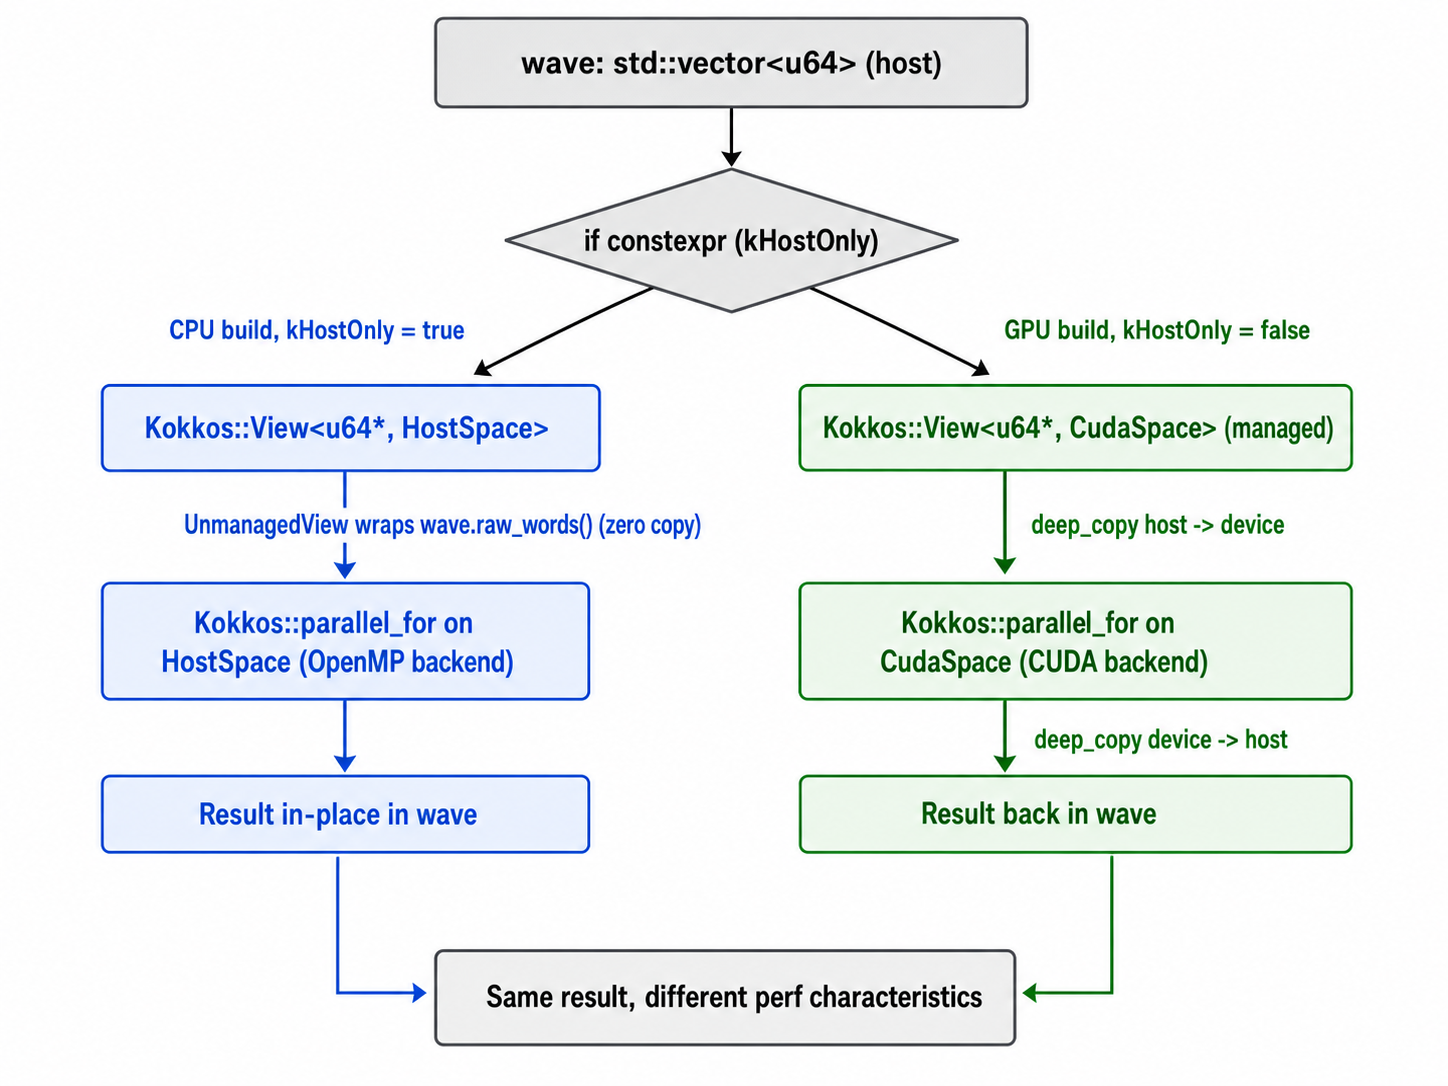
\includegraphics[width=0.85\linewidth]{results/figures/schemas/kokkos_architecture.png}
\caption{Architecture Kokkos pour la propagation BFS, avec branche \texttt{kHostOnly} compile-time choisissant zero-copy ou deep\_copy.}
\label{fig:kokkos_architecture}
\end{figure}

Le backend Kokkos repose sur trois composants :

\begin{enumerate}
    \item \textbf{Vues GPU-accessibles} (\texttt{Kokkos::View<u64*, MemSpace>}) pour la wave et les règles d'adjacence.
    \item \textbf{Fonctor de propagation} (\texttt{PropagateOp}) marqué \texttt{KOKKOS\_INLINE\_FUNCTION}, dispatché par \texttt{Kokkos::parallel\_for}.
    \item \textbf{Branche \texttt{kHostOnly} compile-time} qui choisit zero-copy (CPU build) ou \texttt{deep\_copy} (GPU build).
\end{enumerate}

\subsection{Détection compile-time du backend}

\begin{lstlisting}[language=C++]
using ExecSpace = Kokkos::DefaultExecutionSpace;
using MemSpace = ExecSpace::memory_space;

// True quand le memory space par défaut est HostSpace (build CPU OpenMP).
// False sur build CUDA / HIP (memory space sur device).
constexpr bool kHostOnly = std::is_same<MemSpace, Kokkos::HostSpace>::value;
\end{lstlisting}

Cette constexpr permet ensuite de choisir entre zero-copy et deep\_copy via \texttt{if constexpr} :

\begin{lstlisting}[language=C++]
if constexpr (kHostOnly) {
    // Wrap directement le buffer host de Wave (zero-copy)
    s.wave_view = U64View(wave.raw_words(), wave.total_words());
} else {
    // Buffer device séparé, deep_copy host -> device
    s.wave_view = U64View("wfc_wave", wave.total_words());
    Kokkos::deep_copy(s.wave_view, host_wave_view);
}
\end{lstlisting}

\textbf{Conséquence} : le build CPU paie zéro overhead (le compilateur évalue \texttt{kHostOnly = true} et inline directement). Le build GPU paie la copie host↔device, mais c'est inévitable sur cette architecture.

% =============================================================================
\section{Stack arrays plutôt que heap dans le kernel}
\label{sec:kokkos:stack_arrays}
% =============================================================================

\begin{important}{Contrainte GPU : pas de heap dans le kernel}
Sur device, l'allocation dynamique (\texttt{new}, \texttt{std::vector::resize}) est soit interdite, soit catastrophique en perf. Le code GPU doit utiliser uniquement des stack arrays de taille connue à la compilation.
\end{important}

Notre solution : \texttt{constexpr std::size\_t MAX\_WORDS\_PER\_CELL = 8} (couvre jusqu'à 512 tuiles, largement suffisant pour nos samples).

\begin{lstlisting}[language=C++, caption={PropagateOp fonctor avec stack arrays}]
struct PropagateOp {
    WaveView_K wave;
    RulesView_K rules;
    IntView frontier;
    IntView next_frontier;
    IntView next_count;
    U8View in_queue;
    IntView contradiction_flag;

    KOKKOS_INLINE_FUNCTION
    void operator()(const int idx) const {
        if (Kokkos::atomic_load(&contradiction_flag(0))) return;

        const int c = frontier(idx);
        const int W = wave.words_per_cell;

        // Stack snapshot anti-race (1 mot pour L<=64, jusqu'a 8)
        std::uint64_t snap[MAX_WORDS_PER_CELL];
        for (int w = 0; w < W; ++w) snap[w] = wave.words(c * W + w);

        for (int dy = ...; ...) for (int dx = ...; ...) {
            const int nc = wave.torus_idx(...);

            // Stack accumulator
            std::uint64_t allowed[MAX_WORDS_PER_CELL];
            for (int w = 0; w < W; ++w) allowed[w] = 0ULL;
            // ... union over snap's set bits ...

            bool changed = false;
            for (int i = 0; i < W; ++i) {
                const u64 mask = allowed[i];
                if (mask == 0xFFFFFFFFFFFFFFFFULL) continue;
                // Relaxed-load skip (mirror OMP optim)
                const u64 cur = Kokkos::atomic_load(&wave.words(nc * W + i));
                if ((cur & ~mask) == 0ULL) continue;
                const u64 old_val = Kokkos::atomic_fetch_and(
                    &wave.words(nc * W + i), mask);
                if ((old_val & ~mask) != 0ULL) changed = true;
            }
            if (changed) { /* CAS dedup, push to next_frontier */ }
        }
    }
};
\end{lstlisting}

% =============================================================================
\section{Optimisations OMP propagées au kernel Kokkos}
\label{sec:kokkos:propagated}
% =============================================================================

Toutes les optimisations validées en OMP ont été propagées au kernel Kokkos :

\begin{table}[H]
\centering
\begin{tabularx}{\textwidth}{lX}
\toprule
\textbf{Optim OMP} & \textbf{Implémentation Kokkos} \\
\midrule
Snapshot anti-race & Stack array \texttt{snap[MAX\_WORDS\_PER\_CELL]} \\
\midrule
Mask all-ones skip & \texttt{if (mask == \textasciitilde{}0ULL) continue;} avant atomic \\
\midrule
Relaxed-load skip avant atomic & \texttt{Kokkos::atomic\_load} puis \texttt{Kokkos::atomic\_fetch\_and} \\
\midrule
CAS dedup sur in\_queue & \texttt{Kokkos::atomic\_compare\_exchange} \\
\midrule
Counter atomique \texttt{next\_frontier} & \texttt{atomic\_fetch\_add(\&next\_count(0), 1)} \\
\bottomrule
\end{tabularx}
\caption{Optimisations OMP transposées au backend Kokkos. Le code device respecte les mêmes invariants algorithmiques.}
\label{tab:kokkos:optims}
\end{table}

% =============================================================================
\section{Cleanup correct : \texttt{push\_finalize\_hook}}
\label{sec:kokkos:cleanup}
% =============================================================================

\begin{important}{Bug subtil rencontré : View deallocated after Kokkos::finalize}
Un solver Kokkos cache des Views dans des variables \texttt{static thread\_local} (rules cache, scratch buffers). À process exit, l'ordre de destruction est : \texttt{Kokkos::finalize()} → variables \texttt{thread\_local}. Le second tente de désallouer des buffers Kokkos après que le memory subsystem a été tear-down. Erreur runtime.
\end{important}

\subsection{Solution : \texttt{push\_finalize\_hook}}

Kokkos fournit \texttt{push\_finalize\_hook} qui enregistre une callback exécutée \textit{pendant} \texttt{Kokkos::finalize}, avant le tear-down.

\begin{lstlisting}[language=C++]
void install_finalize_hook_once() {
    static thread_local bool installed = []() {
        Kokkos::push_finalize_hook([]() {
            clear_rules_cache();
            clear_kokkos_scratch();
        });
        return true;
    }();
    (void)installed;
}
\end{lstlisting}

Avec ce hook, les Views sont libérées dans l'ordre correct : caches statiques d'abord, finalize ensuite.

% =============================================================================
\section{Min-entropy : restée sur CPU}
\label{sec:kokkos:min_entropy_cpu}
% =============================================================================

Une décision de design importante : la sélection min-entropie reste \textbf{sur CPU} dans le backend Kokkos, même quand le backend GPU est actif.

\textbf{Raisons :}
\begin{itemize}
    \item La sélection accède à \texttt{wave.at(c).count()} et \texttt{weighted\_entropy(...)}, qui passent par les méthodes \texttt{Wave::at()} non-portables sur device (Wave est en \texttt{std::vector}, pas device-accessible).
    \item Porter min-entropy sur device exigerait de mirrorer le wave en \texttt{Kokkos::View} pour le scan, puis copier le résultat back. La latence ajoutée annule le bénéfice.
    \item En pratique, la propagation domine le temps GPU (les transferts host↔device par propagate sont le vrai bottleneck, voir Chapitre~\ref{chap:resultats}).
\end{itemize}

Une optimisation future : mirrorer la wave une fois au début du solve et exécuter min-entropy sur device avec un kernel séparé. Documenté dans \texttt{docs/CHOICES.md}.

% =============================================================================
\section{Validation GPU sur Romeo armgpu}
\label{sec:kokkos:gpu_validation}
% =============================================================================

\subsection{Build CUDA}

Sur la partition \texttt{armgpu} de Romeo (NVIDIA GH200, sm\_90), un
script SLURM compile Kokkos avec
\texttt{Kokkos\_ENABLE\_CUDA=ON} et
\texttt{Kokkos\_ARCH\_HOPPER90=ON}, puis link le projet contre cette
installation. Commandes en Annexe~\ref{sec:annexes:build}.

\subsection{Tests GPU}

Avec ce build :
\begin{itemize}
    \item \texttt{wfc\_serial} et \texttt{wfc\_omp} tournent sur ARM CPU comme d'habitude.
    \item \texttt{wfc\_kokkos} lance les kernels CUDA via \texttt{Kokkos::parallel\_for}, exécutés sur la GH200.
    \item Tests unitaires : \texttt{test\_solver\_kokkos} (déterminisme bit-à-bit serial vs Kokkos GPU) passe à 100\%.
\end{itemize}

\subsection{Performance GPU : déception et leçons}

Mesures sur \texttt{binary\_5x5} :

\begin{table}[H]
\centering
\begin{tabular}{lrrrr}
\toprule
\textbf{Taille} & \textbf{aarch64 serial} & \textbf{aarch64 omp t=4} & \textbf{aarch64 omp t=16} & \textbf{GPU GH200 (kokkos)} \\
\midrule
32×32 & 0.010 s & 0.082 s & 0.440 s & 0.173 s \\
64×64 & 0.166 s & 0.341 s & 2.551 s & 0.855 s \\
128×128 & 2.623 s & 1.755 s & 10.255 s & 5.431 s \\
256×256 & --- & --- & --- & 52.1 s \\
\bottomrule
\end{tabular}
\caption{Le GPU GH200 est plus lent que le CPU sur tous les workloads testés.}
\label{tab:kokkos:gpu_perf}
\end{table}

\begin{important}{Le GPU est plus lent que le CPU}
À 128×128, GPU = 5.4 s vs CPU OMP 4t aarch64 = 1.8 s. À 256×256, GPU = 52 s, à comparer aux 7.5 s de OMP 16 threads sur EPYC.
\end{important}

Quatre causes identifiées (analysées en détail au Chapitre~\ref{chap:resultats}) :

\begin{enumerate}
    \item \textbf{H↔D copies par propagate} : \texttt{WFCSolverBase} appelle \texttt{propagate} $\sim 8000$ fois par solve. Chaque appel synchronise host wave → device + device → host. Pour 256×256, c'est 524 KB par sens × 16000 = 16 GB de transfert PCIe. À 25 GB/s c'est 0.6 s rien que de transferts.
    \item \textbf{Pas assez de parallélisme par niveau BFS} : un niveau de 100 cellules sur une GH200 (16 896 cores CUDA) = 99\% des cores oisifs.
    \item \textbf{Atomic contention sur unités globales du GPU} : les \texttt{Kokkos::atomic\_fetch\_and} sur GPU passent par les unités atomiques globales, bien plus lent que les atomics CPU sur cache local.
    \item \textbf{Min-entropie reste sur CPU} : la phase qui domine ($\sim 85\%$ du temps en serial) ne profite pas du GPU.
\end{enumerate}

\subsection{Pour vraiment exploiter le GPU}

Pour rendre WFC réellement plus rapide sur GPU, il faudrait un changement algorithmique :

\begin{itemize}
    \item \textbf{Lancer 32 attempts indépendants en parallèle sur 32 SMs}, retourner le premier succès (multi-instance parallelism).
    \item \textbf{Résoudre plusieurs petits problèmes en parallèle} dans le même kernel (batching).
    \item \textbf{Repenser BFS en frontier-less} / iterative refinement.
\end{itemize}

Ces pistes sont documentées au Chapitre~\ref{chap:limites}. Le port Kokkos GPU reste utile : le code compile et tourne sur GH200, les tests d'invariants passent. Pour la performance pratique sur ce workload, le CPU EPYC 9654 reste le meilleur choix.

% =============================================================================
\section{Récap Kokkos}
\label{sec:kokkos:recap}
% =============================================================================

\begin{itemize}
    \item \textbf{Un seul code source}, compile pour CPU OpenMP et GPU CUDA.
    \item \textbf{Branche compile-time \texttt{kHostOnly}} pour zero-copy CPU et deep\_copy GPU. Pas d'overhead sur build CPU.
    \item \textbf{Stack arrays} pour respecter la contrainte GPU « pas de heap dans le kernel ».
    \item \textbf{Optims OMP propagées} : snapshot, mask all-ones, relaxed-load, CAS dedup, atomic counter.
    \item \textbf{push\_finalize\_hook} pour cleanup correct des caches statiques.
    \item \textbf{Tests} : déterminisme bit-à-bit serial = Kokkos vérifié sur CPU et sur GPU GH200.
    \item \textbf{Perf GPU} décevante sur ce workload, mais le port est correct et fonctionnel. Optimisation algorithmique nécessaire pour vraiment exploiter le GPU.
\end{itemize}


% Chapitre 8 : Extensions algorithmiques (symétries, backtracking, parallel attempts)
\chapter{Extensions algorithmiques}
\label{chap:extensions}

Au-delà du sujet de base, le projet livre quatre extensions optionnelles. Toutes sont \textbf{opt-in} : leur activation se fait via un flag CLI ou une option CMake, et le chemin par défaut reste strictement inchangé en performance.

\section{Parallel attempts : K essais indépendants en parallèle}

\subsection{Motivation}

L'analyse du speedup OMP intra-attempt (Chapitre~\ref{chap:resultats}) révèle un plafonnement : au-delà de 8-16 threads, la parallélisation interne d'un seul attempt sature à cause des barrières BFS et de la contention atomique. Une approche complémentaire : au lieu de paralléliser \textit{dans} un attempt, lancer K attempts \textit{indépendants} en parallèle, chacun avec un seed dérivé différent.

\subsection{Algorithme}

\begin{algorithm}[H]
\caption{Parallel attempts orchestration}
\begin{algorithmic}[1]
\Require Options $opt$ avec $K = opt.\text{parallel\_attempts} > 1$
\For{batch\_start = 0, K, 2K, ... < $opt.\text{max\_attempts}$}
    \State $batch\_size \gets \min(K, opt.\text{max\_attempts} - batch\_start)$
    \State \textbf{parallel for} $k = 0$ \textbf{to} $batch\_size - 1$ \textbf{do}
        \State \quad $seed_k \gets \texttt{attempt\_seed}(opt.\text{seed}, batch\_start + k)$
        \State \quad $success_k \gets \texttt{serial\_run\_attempt}(waves_k, ...)$
    \State \textbf{end parallel for}
    \State $picked \gets$ premier $k$ tel que $success_k$
    \If{$picked \neq -1$}
        \State \Return $waves_{picked}$
    \EndIf
\EndFor
\State \Return échec
\end{algorithmic}
\end{algorithm}

\subsection{Garantie de déterminisme}

\begin{theorem}[Déterminisme parallel-attempts]
Pour un même seed initial, \texttt{parallel\_attempts=K} produit la même sortie qu'un retry séquentiel avec \texttt{max\_attempts=K}.
\end{theorem}

\begin{proof}
Le succès d'index minimum dans un batch $[0, K)$ est exactement le premier $k$ tel que $success_k$, qui est précisément le premier seed essayé par le retry séquentiel. Si tous échouent, on passe au batch suivant, qui correspond aux attempts $K \ldots 2K-1$, etc. CQFD.
\end{proof}

Vérifié par \texttt{test\_parallel\_attempts} : K=8 sur sample facile pointe \texttt{attempts == 1} (lowest-success), output bit-identique à un run séquentiel.

\subsection{Bypass du backend pour éviter l'oversubscription}

Chaque attempt parallèle utilise \texttt{serial\_run\_attempt} (de SolverCommon), \textbf{pas} le \texttt{propagate} du backend. Sinon, $K$ attempts × $T$ threads intra-attempt = $K \cdot T$ threads pour $T$ cores → catastrophe.

\subsection{Mesures}

Sur \texttt{terrain N=3 24×24}, total wallclock pour 4 seeds (Windows i9-10900K) :

\begin{table}[H]
\centering
\begin{tabular}{lrr}
\toprule
\textbf{Mode} & \textbf{Total} & \textbf{Speedup} \\
\midrule
sequential, 1 thread & 0.510 s & 1.0× \\
\texttt{--parallel-attempts 4 --threads 4} & 0.332 s & 1.54× \\
\texttt{--parallel-attempts 8 --threads 8} & 0.238 s & \textbf{2.14×} \\
\bottomrule
\end{tabular}
\caption{Parallel attempts : 2.14× wallclock sur workload à fort taux de retry.}
\label{tab:ext:parallel_attempts}
\end{table}

\subsection{Quand utiliser}

\begin{itemize}
    \item \textbf{Paie} sur les workloads à fort taux d'échec par attempt (terrain N=3 où ~10\% de succès par seed).
    \item \textbf{Inutile} sur les workloads qui réussissent du premier coup (binary\_5x5, smooth\_N3) : K attempts en parallèle = K× le travail pour le même résultat.
\end{itemize}

% =============================================================================
\section{Symétries D4 : expansion du tile set}
\label{sec:ext:symmetries}
% =============================================================================

\subsection{Motivation}

Le sujet et l'article de référence \cite{heaton2018wfc} mentionnent que le tile set peut être étendu par rotations / réflexions. Cette extension est utile sur des samples avec une orientation préférée (chemins, escaliers, branchages) : on veut que le motif s'applique uniformément dans toutes les orientations dans la sortie.

\subsection{Le groupe diédral $D_4$}

\begin{definition}[Groupe $D_4$]
Le groupe diédral d'ordre 8, $D_4$, est le groupe des symétries du carré : 4 rotations (0°, 90°, 180°, 270°) et 4 réflexions (axiales et diagonales).
\end{definition}

\begin{table}[H]
\centering
\begin{tabular}{cl}
\toprule
$S$ & Variantes générées par tuile \\
\midrule
1 & identité (défaut, comportement legacy) \\
2 & identité + rotation 180° \\
4 & 4 rotations \\
8 & 4 rotations + 4 réflexions ($D_4$ complet) \\
\bottomrule
\end{tabular}
\caption{Niveaux d'expansion D4 supportés par \texttt{TileSet::from\_sample(grid, N, S)}.}
\label{tab:ext:symmetries_levels}
\end{table}

\subsection{Implémentation}

\texttt{Tile::rotated\_90()} et \texttt{Tile::reflected\_horizontal()} sont des helpers purs qui retournent un nouveau \texttt{Tile}. Pour chaque pattern extrait, on génère ses variantes et on les déduplique par hash de contenu :

\begin{lstlisting}[language=C++]
template <typename Emit>
void emit_variants(const Tile& t, int symmetries,
                   std::unordered_map<Tile, int, TileHash>& seen,
                   Emit emit) {
    auto try_emit = [&](Tile&& v) {
        if (seen.find(v) != seen.end()) return;
        seen.emplace(v, 0);
        emit(std::move(v));
    };
    try_emit(Tile{t});
    if (symmetries == 1) return;
    Tile r90  = t.rotated_90();
    Tile r180 = r90.rotated_90();
    Tile r270 = r180.rotated_90();
    if (symmetries >= 2) try_emit(std::move(r180));
    if (symmetries >= 4) {
        try_emit(std::move(r90));
        try_emit(std::move(r270));
    }
    if (symmetries >= 8) {
        try_emit(t.reflected_horizontal());
        try_emit(t.rotated_90().reflected_horizontal());
        try_emit(r180.reflected_horizontal());
        try_emit(r270.reflected_horizontal());
    }
}
\end{lstlisting}

\subsection{Hot path inchangé à $S=1$}

À $S = 1$ (défaut), \texttt{from\_sample} suit exactement le code legacy :

\begin{lstlisting}[language=C++]
if (symmetries == 1) {
    auto [it, inserted] = index.try_emplace(...);
    // ... pas de génération de variantes, identique au legacy
} else {
    // ... expansion via emit_variants
}
\end{lstlisting}

Vérifié bit-à-bit par \texttt{test\_symmetries} : \texttt{from\_sample(g, N)} (legacy 2-args) produit le même TileSet que \texttt{from\_sample(g, N, 1)} (3-args explicite).

\subsection{Effet sur le tile set}

\begin{table}[H]
\centering
\begin{tabular}{lrrrr}
\toprule
\textbf{Sample} & \textbf{S=1} & \textbf{S=2} & \textbf{S=4} & \textbf{S=8} \\
\midrule
\texttt{skyline N=3} & 79 & 142 & 247 & 331 \\
\texttt{plant N=3} & 94 & 172 & 335 & 403 \\
\texttt{rooms N=3} & 14 & 14 & 14 & 14 \\
\bottomrule
\end{tabular}
\caption{Croissance du tile set selon $S$. Les patterns auto-symétriques (rooms binaire avec rotation/réflexion équivalentes) ne sont pas dupliqués.}
\label{tab:ext:tile_count}
\end{table}

L'auto-symétrie est gérée correctement : un sample uniformément peuplé de zéros, ou un damier, donne 1 tuile à $S = 1, 2, 4, 8$.

\subsection{Coût}

L'expansion se fait \textbf{une fois à l'extraction} (quelques µs même pour gros samples). Le solveur ne sait pas que les tuiles viennent de symétries, il voit juste un $L$ plus grand.

\textbf{Effet indirect} : $L'$ peut passer de 11 à 88 → bitsets parfois à 2 mots → solveur $\sim 1.5\times$ plus lent. Cohérent : plus de variantes = plus de choix par cellule.

% =============================================================================
\section{Backtracking avec snapshot delta-encodé}
\label{sec:ext:backtracking}
% =============================================================================

\subsection{Motivation}

Sur les samples très contraints (terrain N=3 sur petite grille), restart-on-contradiction épuise rapidement \texttt{max\_attempts} sans trouver de solution. Le backtracking, opt-in via \texttt{--backtrack}, explore l'arbre de recherche au lieu d'abandonner.

\subsection{Algorithme}

\begin{algorithm}[H]
\caption{Backtracking avec snapshot delta-encodé}
\begin{algorithmic}[1]
\State $stack \gets \emptyset$
\Loop
    \State $cell \gets \texttt{serial\_min\_entropy}()$
    \If{$cell < 0$}
        \State \Return succès
    \EndIf
    \State Ouvrir frame $F = \{cell, \text{candidates triés par fréquence desc}, \emptyset\}$
    \State Push $F$ sur $stack$
    \If{$\texttt{try\_top}(stack)$}
        \State Continue \Comment{forward}
    \EndIf
    \State $stack.\textsc{Pop}()$
    \While{$stack \neq \emptyset$}
        \State $\texttt{apply\_inverse}(stack.top.delta)$ \Comment{undo last try}
        \If{$\texttt{try\_top}(stack)$}
            \State Break \Comment{recovered}
        \EndIf
        \State $stack.\textsc{Pop}()$
    \EndWhile
    \If{$stack = \emptyset$}
        \State \Return échec
    \EndIf
\EndLoop
\end{algorithmic}
\end{algorithm}

\subsection{Optim 1 : Delta-encoded snapshot}

\begin{important}{Snapshot delta plutôt que snapshot complet}
Chaque frame ne stocke que les cellules effectivement modifiées par sa propagation. Mémoire : $\sim 50 \cdot W \cdot 16$ octets par frame (vs $r \cdot c \cdot W \cdot 8$ pour un snapshot plein), $\sim 80\times$ moins sur 64×64 binaire.
\end{important}

Implémentation : \texttt{serial\_propagate\_with\_delta} peek le pre-state en stack scratch, commit dans le delta uniquement si \texttt{and\_with} mute la cellule. Un flag \texttt{touched} évite le double-recording.

\begin{lstlisting}[language=C++]
struct WaveDelta {
    int words_per_cell = 0;
    std::vector<int> cells;
    std::vector<u64> before;
};

void apply_delta(Wave& wave, const WaveDelta& delta) {
    const int W = delta.words_per_cell;
    for (size_t k = 0; k < delta.cells.size(); ++k) {
        u64* dst = wave.raw_words() + delta.cells[k] * W;
        const u64* src = delta.before.data() + k * W;
        for (int w = 0; w < W; ++w) dst[w] = src[w];
    }
}
\end{lstlisting}

\subsection{Optim 2 : Composition avec parallel-attempts}

\texttt{solve\_parallel} détecte \texttt{use\_backtracking=true} et lance K recherches backtrack indépendantes, chacune avec un seed dérivé (donc ordre de tie-break différent → arbre d'exploration différent). Le succès d'index minimum gagne.

C'est la forme classique de \textit{parallel backtracking via independent searches} : pas de partage d'état entre recherches, pas de work stealing, donc simple et correct.

\subsection{Choix triés par fréquence descendante}

À chaque frame, les candidats sont triés par fréquence descendante : la tuile la plus probable est essayée en premier (heuristique « try the most likely »). Le backtracking est \textbf{déterministe} pour un seed donné, mais le seed influence l'ordre via \texttt{cell\_jitter} (entropy ties).

\subsection{Bypass du backend parallèle intra-attempt}

Le snapshot/restore n'a de sens qu'en single-threaded. Quand \texttt{use\_backtracking=true}, \texttt{solve\_sequential} invoque directement \texttt{serial\_run\_attempt\_backtrack} au lieu de la dispatch backend. Combiner backtrack + OMP intra-attempt ouvrirait des races inutilement complexes.

\subsection{Mesures}

\begin{table}[H]
\centering
\begin{tabular}{lrr}
\toprule
\textbf{Configuration} & \textbf{Temps} & \textbf{Résultat} \\
\midrule
\texttt{terrain N=3 32×32} retry-30 attempts & 0.38 s & \textbf{ÉCHEC} \\
\texttt{terrain N=3 32×32} \texttt{--backtrack} & 0.12 s & \textbf{succès} \\
\texttt{terrain N=3 32×32} \texttt{--parallel-attempts 8 --backtrack} & 0.20 s & succès \\
\bottomrule
\end{tabular}
\caption{Backtracking résout des instances où retry échoue. Le parallel-bt est plus lent ici car le single-bt trouve déjà vite (overhead K parallèle inutile sur ce cas).}
\label{tab:ext:backtrack}
\end{table}

% =============================================================================
\section{Démo Unreal Engine 5 : \texttt{wfc\_dungeon}}
\label{sec:ext:ue5}
% =============================================================================

\subsection{Motivation}

WFC est massivement utilisé pour la génération de niveaux dans les jeux. Pour démontrer que notre solveur s'intègre dans un pipeline réaliste, nous livrons une cible CLI \texttt{wfc\_dungeon} qui émet un JSON consommé par un plugin Unreal Engine 5.7.

\subsection{Pipeline}

\begin{figure}[H]
\centering
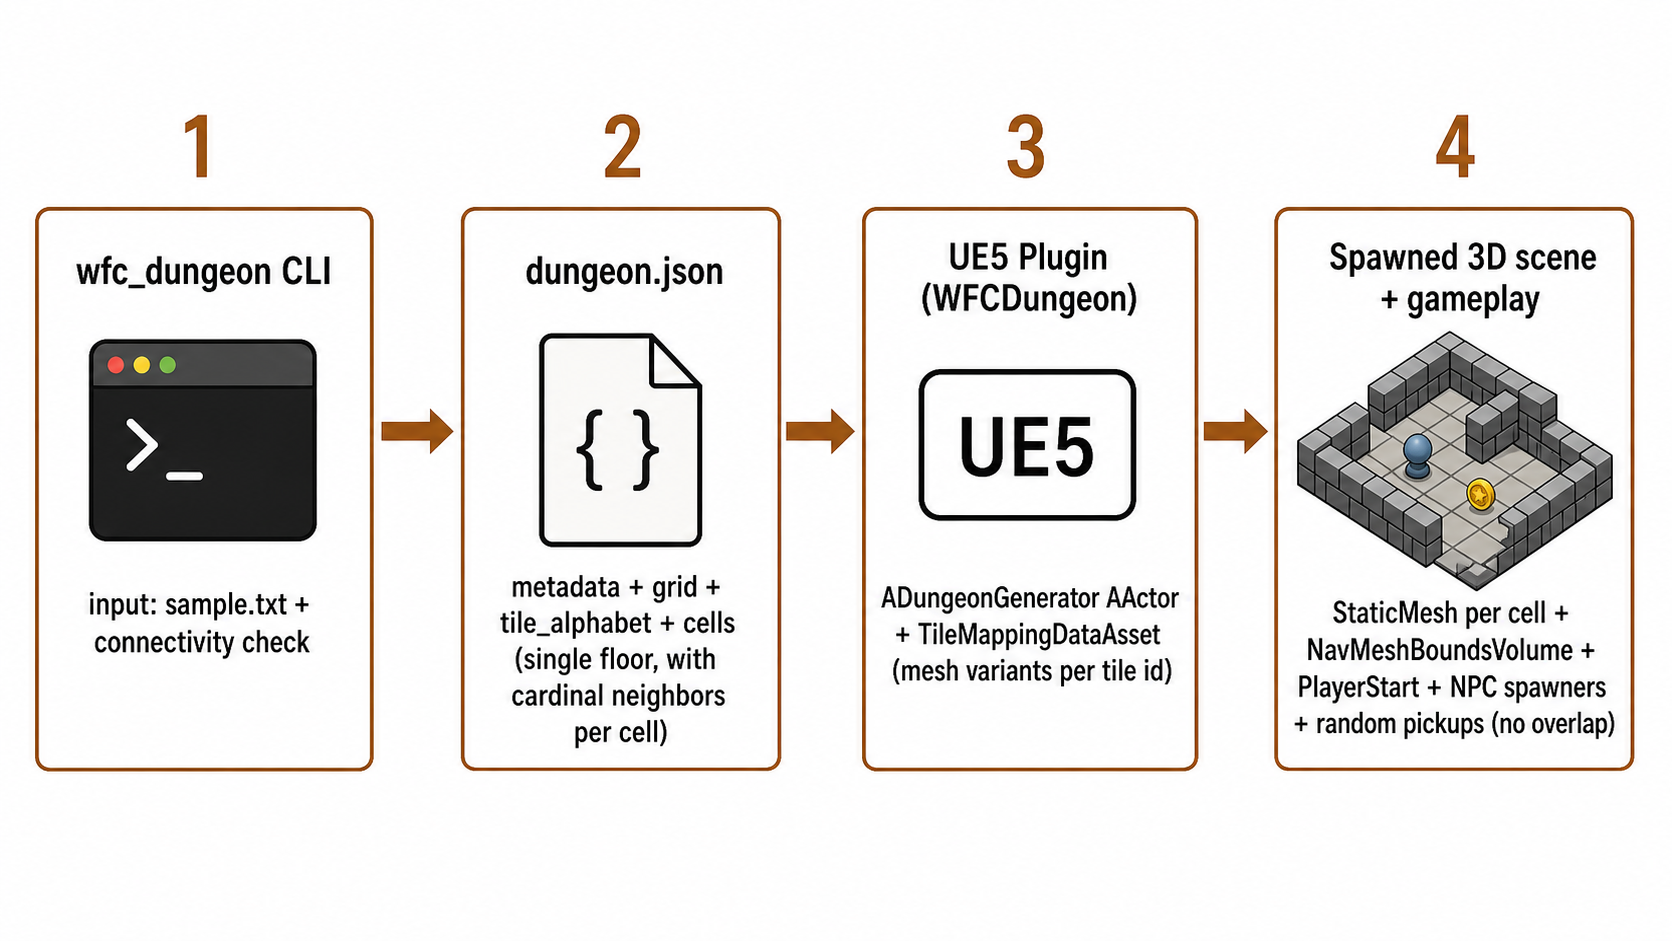
\includegraphics[width=0.95\linewidth]{results/figures/schemas/ue5_pipeline.png}
\caption{Pipeline asset → JSON → spawn de meshes UE5 + gameplay actors.}
\label{fig:ue5_pipeline}
\end{figure}

\subsection{Format JSON}

\begin{lstlisting}[language=C++]
{
  "version": 1,
  "metadata": { "sample": "...", "N": 2, "seed": 42 },
  "grid": { "rows": 24, "cols": 24, "cell_size_cm": 200,
            "wall_height_cm": 300 },
  "tile_alphabet": [ {"id": 0, "name": "floor"}, ... ],
  "cells": [
    { "row": 0, "col": 0, "tile_id": 0, "tile_name": "floor",
      "neighbors": { "n": 1, "s": 0, "e": 1, "w": 1 } },
    ...
  ]
}
\end{lstlisting}

Le pipeline est strictement \textbf{single-floor}. Une version
antérieure proposait un schéma v2 multi-étages avec auto-placement
d'escaliers ; le plugin UE5 a été simplifié pour coller au cas
mono-étage qui couvre les besoins de la démo, et le code mort
correspondant (flags \texttt{--levels}, \texttt{--floor-height},
\texttt{--stair-id}, struct \texttt{LevelGrid}, \texttt{place\_stairs},
branche multi-floor de \texttt{write\_dungeon\_json}) a été retiré.

\subsection{Connectivité par flood-fill BFS}

Avant d'émettre le JSON, \texttt{wfc\_dungeon} vérifie que les cellules
\textit{walkable} forment une composante connexe (flood-fill BFS). Si
plusieurs composantes sont détectées, l'algorithme re-roll avec un
nouveau seed (jusqu'à \texttt{--connectivity-attempts} fois). Garantit
qu'un joueur peut traverser tout le niveau.

\subsection{Plugin UE 5.7}

Le plugin \texttt{ue5\_plugin/WFCDungeon/} contient :

\begin{itemize}
    \item \texttt{UTileMappingDataAsset} : mappe chaque \texttt{tile\_id} vers un struct \{floor, wall, corner, door, plus arrays \texttt{*MeshVariants}\} + flags \texttt{bIsSolid}/\texttt{bIsDoor} + offset/scale. Les variants permettent un \textit{random pick} par tile id (fallback single-mesh).
    \item \texttt{ADungeonGenerator} : AActor qui parse le JSON, walk les cells, et spawne les \texttt{StaticMeshComponent} avec yaw cardinal (-90°N, +90°S, 0°E, 180°W).
\end{itemize}

\subsection{Gameplay actors et navmesh}

\texttt{ADungeonGenerator} expose des slots \texttt{TSubclassOf<AActor>}
pour transformer le dungeon en scaffold gameplay :

\begin{itemize}
    \item \texttt{PlayerStartClass} : 4 cellules walkable les plus proches du centre.
    \item \texttt{CornerSpawnerClass} (NPC) : scattered sur \texttt{NumCornerSpawners} cellules.
    \item \texttt{RandomPickupClass} : scattered sur \texttt{NumRandomPickups} cellules.
    \item Allocation non-collisionnelle : aucune cellule n'héberge deux catégories.
    \item Z-offsets dédiés (\texttt{GameplayActorZOffsetCm}, \texttt{PlayerStartZOffsetCm}) pour positionner les capsules au-dessus du sol.
\end{itemize}

\textbf{Volume de navigation auto-calculé} : un
\texttt{ANavMeshBoundsVolume} est spawné automatiquement, dimensionné
sur toute la grille via \texttt{UCubeBuilder} en éditeur (les polygones
de la brush sont reconstruits pour matcher visuellement le dungeon).
En runtime, fallback sur le scaling de l'actor.

\textbf{Bouton \textit{Generate Random}} : un appel
\textit{CallInEditor} qui spawn \texttt{wfc\_dungeon.exe} en
sous-processus avec un seed frais, écrit le JSON dans
\texttt{Saved/WFCTemp}, et chaîne le parsing immédiat. Une seule action
pour générer un nouveau dungeon.

\textbf{Périmètre fermé} : le flag \texttt{bWallOnBorders} (true par
défaut) ferme le pourtour du dungeon avec des walls, ce qui est utile
pour empêcher le joueur de sortir de la zone walkable.

\subsection{Build opt-in}

\texttt{-DBUILD\_DUNGEON=ON} active la cible \texttt{wfc\_dungeon}.
Sans, la cible n'est pas générée du tout (vérifié :
\texttt{ninja: no work to do} après reconfigure). Aucun impact sur le
benchmark, les ctests, ou les solveurs parallèles.

\subsection{Captures écran du dungeon généré}
\label{sec:ext:ue5:screens}

Trois captures du dungeon généré par \texttt{wfc\_dungeon} puis spawné dans
UE 5.7 par le plugin \texttt{ADungeonGenerator}. Le grid binaire
(\texttt{rooms.txt}, $N=2$, 24×24) est résolu par le solveur, sérialisé
en JSON, puis chaque cellule \textit{walkable} est instanciée comme
\texttt{StaticMeshComponent} (sol + variants) tandis que les cellules
\textit{solid} bordant un walkable spawnent un wall mesh avec yaw
cardinal correct.

\begin{figure}[H]
\centering
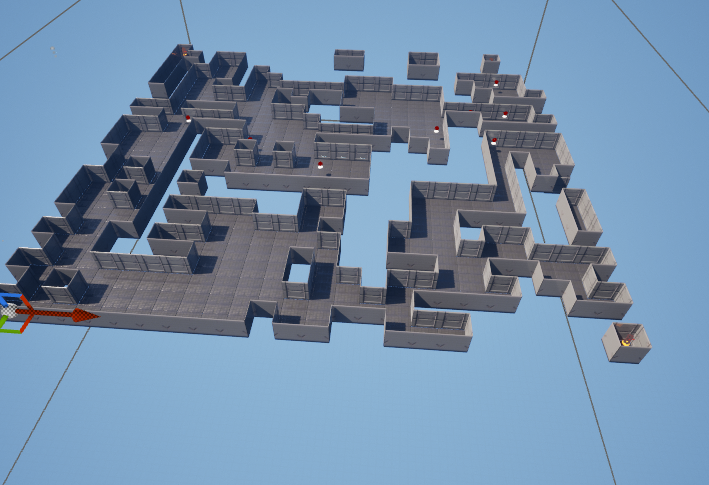
\includegraphics[width=0.95\linewidth]{results/figures/ue5/ue5_dungeon_01.png}
\caption{Vue d'ensemble du dungeon : grille 24×24 résolue par WFC,
spawnée en 3D avec sols texturés, walls, et périmètre fermé
(\texttt{bWallOnBorders=true}). Les pickups sont visibles sur
plusieurs cellules walkable.}
\label{fig:ue5_dungeon_01}
\end{figure}

\begin{figure}[H]
\centering
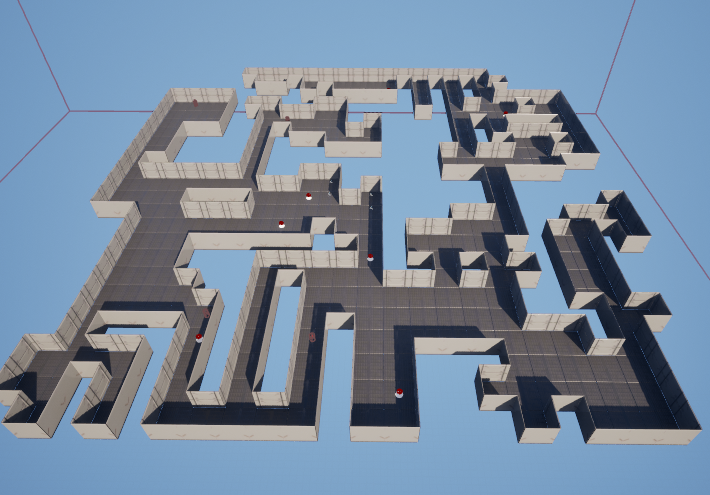
\includegraphics[width=0.95\linewidth]{results/figures/ue5/ue5_dungeon_02.png}
\caption[Détail d'une intersection de couloirs.]{Détail d'une
intersection de couloirs : les meshes de sol sont choisis
aléatoirement parmi \texttt{FloorMeshVariants} (variation visuelle),
les walls sont orientés selon leurs voisins walkable. La
connectivité globale walkable a été validée par flood-fill BFS
avant spawn.}
\label{fig:ue5_dungeon_02}
\end{figure}

\begin{figure}[H]
\centering
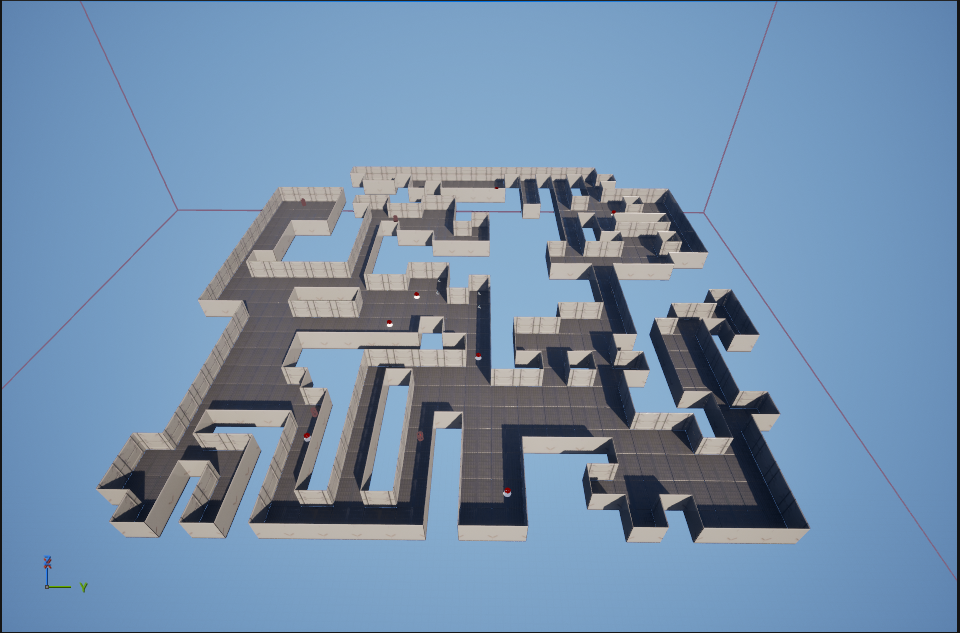
\includegraphics[width=0.95\linewidth]{results/figures/ue5/ue5_dungeon_03.png}
\caption[Vue d'une pièce avec PlayerStart, NPC et pickups.]{Vue
d'une pièce avec un \texttt{APlayerStart} (capsule), un NPC spawner
et plusieurs pickups. L'allocation non-collisionnelle garantit
qu'aucune cellule walkable n'héberge deux catégories d'actors. Le
\texttt{ANavMeshBoundsVolume} couvre toute la grille pour la
navigation IA.}
\label{fig:ue5_dungeon_03}
\end{figure}


% Chapitre 9 : Protocole expérimental (benchmarking)
\chapter{Protocole expérimental et benchmarking}
\label{chap:protocole}

Ce chapitre décrit la méthodologie expérimentale : plates-formes de mesure, samples utilisés, métriques calculées, scripts SLURM, et reproductibilité.

\section{Plates-formes}
\label{sec:proto:plateformes}

\begin{table}[H]
\centering
\begin{tabularx}{\textwidth}{lXll}
\toprule
\textbf{ID} & \textbf{Hardware} & \textbf{OS} & \textbf{Compilateur} \\
\midrule
\texttt{lin-i9} & Intel i9-10900K (10c/20t HT) & Ubuntu 24.04 / WSL2 & g++ 13.3, OpenMP 4.5 \\
\texttt{win-i9} & Intel i9-10900K & Windows 11 + MSYS2 MinGW & g++ 16.1, OpenMP 5.2 \\
\texttt{romeo} & AMD EPYC 9654 (192c, 8 NUMA) & RHEL 9 & g++ 14.2, OpenMP 4.5 \\
\texttt{romeo-gpu} & ARM Neoverse-V2 + NVIDIA GH200 & RHEL 9 & g++ 11.4 + nvcc 12.9 \\
\bottomrule
\end{tabularx}
\caption{Plates-formes utilisées pour les benchmarks. Romeo est la cible HPC principale.}
\label{tab:proto:plateformes}
\end{table}

\subsection{Romeo, plate-forme cible}

Le supercalculateur \textbf{Romeo} de l'Université de Reims Champagne-Ardenne dispose de plusieurs partitions :
\begin{itemize}
    \item \texttt{x64cpu} : nœuds AMD EPYC 9654, 192 cœurs par nœud, 8 NUMA nodes (3 CCDs par node, 8 cœurs par CCD), 768 GB DRAM.
    \item \texttt{armgpu} : 1 nœud ARM Grace + GPU NVIDIA GH200 120 GB HBM3, 132 SMs (16 896 cœurs CUDA).
    \item \texttt{instant} (interactif) et \texttt{short} (jobs < 4h) : utilisés pour nos sweeps.
\end{itemize}

\subsection{Configuration NUMA et threading}

Variables d'environnement utilisées sur Romeo :
\begin{lstlisting}[language=bash]
export OMP_PROC_BIND=close
export OMP_PLACES=cores
\end{lstlisting}

\textbf{Justification :} \texttt{close} place les threads contigus dans la topologie (même CCD avant de passer au CCD suivant), ce qui maximise la localité L3. \texttt{cores} évite l'hyper-threading (1 thread par cœur physique).

\section{Samples utilisés}
\label{sec:proto:samples}

\begin{table}[H]
\centering
\begin{tabularx}{\textwidth}{llXX}
\toprule
\textbf{Sample} & \textbf{$N$} & \textbf{$L$} & \textbf{Caractéristiques} \\
\midrule
\texttt{binary\_5x5} & 2 & 11 & Exemple littéral du sujet, 5×5 binaire \\
\texttt{binary\_stripes} & 2 & 4 & Bandes verticales, très contraint \\
\texttt{binary\_dots} & 2 & 7 & 1 isolés sur fond 0 \\
\texttt{binary\_checker} & 2 & 2 & Damier, dégénéré \\
\texttt{multivalue\_terrain} & 2 & 33 & 4 valeurs (eau/sable/herbe/roche) \\
\texttt{multivalue\_terrain} & 3 & 73 & Idem, $N$=3, contraintes serrées \\
\texttt{multivalue\_maze} & 2 & 24 & 3 valeurs (sol/mur/porte) \\
\texttt{multivalue\_smooth} & 3 & 12 & Gradients lisses, peu de tuiles \\
\texttt{skyline} & 3 & 79 & Skyline urbain, 4 valeurs (gallery WFC) \\
\texttt{plant} & 3 & 94 & Plante avec fleurs, 4 valeurs (gallery) \\
\texttt{rooms} & 3 & 14 & Dungeon binaire, pièces rectangulaires \\
\bottomrule
\end{tabularx}
\caption{Samples couverts par les benchmarks. Trois axes : alphabet (binaire vs multi-valeurs), $N$ (taille de tuile), nombre de tuiles uniques $L$.}
\label{tab:proto:samples}
\end{table}

Les rendus PNG des samples sont présentés en regard de leurs sorties
au Chapitre~\ref{chap:resultats} (Section~\ref{sec:res:gallery}).

\subsection{Workloads agrégés}

Pour les sweeps Romeo, nous regroupons en \textbf{labels} :

\begin{itemize}
    \item \texttt{binary\_L11} : \texttt{binary\_5x5.txt} avec $N=2$, $L=11$. Cas de référence du sujet.
    \item \texttt{binary\_optim} : idem avec optim « frontier-threshold » activée. A/B vs \texttt{binary\_L11}.
    \item \texttt{terrain\_L33} : \texttt{multivalue\_terrain.txt} avec $N=2$, $L=33$.
    \item \texttt{smooth\_N3} : \texttt{multivalue\_smooth.txt} avec $N=3$, $L=12$.
    \item \texttt{binary\_gpu}, \texttt{terrain\_gpu} : mêmes samples sur backend Kokkos CUDA (GH200).
\end{itemize}

\section{Métriques mesurées}
\label{sec:proto:metriques}

\subsection{Temps mesurés}

\begin{table}[H]
\centering
\begin{tabularx}{\textwidth}{lX}
\toprule
\textbf{Métrique} & \textbf{Sémantique} \\
\midrule
\texttt{seconds\_total} & Wall-clock entre l'entrée et la sortie de \texttt{solve()} \\
\texttt{seconds\_solve} & Somme des temps des \texttt{run\_attempt} (vrai temps WFC) \\
\texttt{collapses} & Nombre de cellules décidées \\
\texttt{propagations} & Nombre d'événements de propagation \\
\texttt{attempts} & Nombre d'attempts essayés (1 si succès au premier coup) \\
\bottomrule
\end{tabularx}
\caption{Métriques de \texttt{SolverStats}. \texttt{seconds\_solve} est utilisée comme référence pour les speedup.}
\label{tab:proto:stats}
\end{table}

\subsection{Métriques dérivées}

\begin{itemize}
    \item \textbf{Speedup} : $S(p) = T_{\text{serial}} / T(p)$.
    \item \textbf{Efficacité parallèle} : $E(p) = S(p) / p$.
    \item \textbf{Throughput} : cellules / seconde.
    \item \textbf{Fit Amdahl} : régression non-linéaire de $S(p) = 1 / ((1-f) + f/p)$ ; donne $f$ et $R^2$.
\end{itemize}

\subsection{Réduction du bruit de mesure}

Chaque configuration est mesurée \textbf{3 fois} (paramètre \texttt{--repeats 3}). On reporte la \textbf{médiane}, plus robuste que la moyenne face aux outliers.

Pour les A/B testing fins, on utilise une \textbf{médiane sur 11 runs alternés} : exécution alternée A B A B A B A B A B A, médiane des 6 mesures de chaque variante.

\section{Scripts SLURM Romeo}
\label{sec:proto:slurm}

\begin{table}[H]
\centering
\begin{tabularx}{\textwidth}{lX}
\toprule
\textbf{Script} & \textbf{Rôle} \\
\midrule
\texttt{romeo\_smoke.slurm} & Smoke test 15 min, 32 cores \\
\texttt{romeo\_full\_bench.slurm} & Full sweep CPU 1h, sizes 32-256, threads 1-192 \\
\texttt{romeo\_complement\_bench.slurm} & Complément terrain et smooth, 10 min \\
\texttt{romeo\_optim\_test.slurm} & A/B « frontier-threshold » \\
\texttt{build\_kokkos\_gpu\_romeo.slurm} & Build Kokkos+CUDA + tests sur \texttt{armgpu} \\
\texttt{romeo\_gpu\_bench.slurm} & Bench GPU GH200, 10 min \\
\texttt{romeo\_parallel\_attempts.slurm} & A/B \texttt{--parallel-attempts} sur terrain N=3 \\
\bottomrule
\end{tabularx}
\caption{Scripts SLURM Romeo du projet.}
\label{tab:proto:slurm}
\end{table}

\section{Format CSV des résultats}
\label{sec:proto:csv}

Le \texttt{wfc\_benchmark} émet un CSV avec les colonnes :
\begin{verbatim}
label, backend, threads, sample, N, rows, cols,
seed, repeat, success, attempts, collapses,
propagations, rules_s, solve_s, total_s
\end{verbatim}

Une ligne par (label, backend, threads, size, seed, repeat). Plusieurs labels peuvent coexister dans un même CSV via \texttt{--no-header} sur les sweeps successifs.

\section{Pipeline d'analyse Python}
\label{sec:proto:pipeline}

Une fois le CSV récupéré (\texttt{scp romeo:results/full\_543692.csv ./results/}), un pipeline Python génère figures et tableaux :

\begin{lstlisting}[language=bash]
bash scripts/post_job_pipeline.sh 543692
\end{lstlisting}

\textbf{Scripts Python} :
\begin{itemize}
    \item \texttt{plot\_results.py} : speedup, efficacité, heatmap, throughput, comparaison backends
    \item \texttt{amdahl\_fit.py} : fit non-linéaire, sortie JSON + figures
    \item \texttt{benchmark\_summary.py} : tableaux markdown auto-générés
    \item \texttt{benchmark\_insights.py} : détection automatique des knees, peak, régressions
    \item \texttt{plot\_optim\_compare.py} : barres avant/après pour les A/B
\end{itemize}

\section{Reproductibilité}
\label{sec:proto:reproductibilite}

\begin{itemize}
    \item Scripts SLURM, scripts Python, samples : tous versionnés dans le dépôt git.
    \item Seeds RNG fixés (\texttt{--seed 42}) : exécution déterministe.
    \item CSV bruts commités : on peut re-générer les figures sans relancer Romeo.
    \item Figures finales dans \texttt{docs/figures/} : le rapport compile sans relancer le pipeline.
\end{itemize}

\section{Couverture des configurations}
\label{sec:proto:coverage}

Les 220+ runs benchmarkés sur Romeo couvrent :

\begin{table}[H]
\centering
\begin{tabularx}{\textwidth}{lXX}
\toprule
\textbf{Job ID} & \textbf{Workload} & \textbf{Configuration} \\
\midrule
\texttt{543692} & binary\_L11 sweep 1 & sizes 32-256 ; threads 1-192 \\
\texttt{544061} & terrain\_L33, smooth\_N3 & sizes 32-128 ; threads 1-32 \\
\texttt{544356} & binary\_optim A/B & size 128 ; threads 1-192 \\
\texttt{544361} & binary\_gpu, terrain\_gpu & sizes 32-256 ; threads 1, 4, 16 + GPU \\
\bottomrule
\end{tabularx}
\caption{Jobs SLURM utilisés pour le rapport. CSV combiné de 398 lignes.}
\label{tab:proto:jobs}
\end{table}


% Chapitre 10 : Résultats et analyse
\chapter{Résultats et analyse}
\label{chap:resultats}

Ce chapitre présente les résultats expérimentaux et leur analyse. Nous suivons le flux : validation de la correction, performance séquentielle de référence, scaling OpenMP, fits Amdahl, varying datasets, varying configurations, comparaison Kokkos CPU + GPU, et synthèse des optimisations testées en A/B.

% =============================================================================
\section{Validation : déterminisme bit-à-bit}
\label{sec:res:validation}
% =============================================================================

Avant toute mesure de performance, nous validons que les trois backends produisent un \textbf{output bit-identique} pour un même seed. C'est une exigence forte qui contraint la conception (jitter d'entropie déterministe, réduction min-entropie ordonnée, atomics relaxed associatives).

\subsection{Tests automatisés}

\begin{table}[H]
\centering
\begin{tabularx}{\textwidth}{lrl}
\toprule
\textbf{Suite de tests} & \textbf{Checks} & \textbf{Couverture} \\
\midrule
\texttt{test\_bitset} & 310 & set/clear/and/or/popcount/multi-mots \\
\texttt{test\_grid} & 778 & accès, torus, fill\_row\_major, edge cases \\
\texttt{test\_grid\_io} & 70 & round-trip txt, PNG, PPM, parsing erreurs \\
\texttt{test\_tileset} & 132 & extraction, fréquences, déduplication \\
\texttt{test\_overlap} & 4898 & identité, symétrie, multivalue \\
\texttt{test\_wave} & 8594 & superposition, accesseurs, indépendance \\
\texttt{test\_solver\_common} & 9060 & entropy, weighted\_pick, jitter, build\_output \\
\texttt{test\_solver} & 71 & end-to-end serial, déterminisme, soundness \\
\texttt{test\_edge\_cases} & 404 & failure paths, scale<1, retry exhaustion \\
\texttt{test\_parallel\_attempts} & 16 & lowest-success determinism, retry boost \\
\texttt{test\_symmetries} & 66 & rotated\_90⁴ = id, reflected² = id, monotonic \\
\texttt{test\_backtrack} & 520 & soundness, succès tight, déterminisme \\
\texttt{test\_solver\_omp} & 36 & déterminisme OMP, contradiction, multivalue \\
\texttt{test\_solver\_kokkos} & 22 & déterminisme Kokkos serial vs Kokkos \\
\texttt{test\_kokkos\_autoinit} & 3 & init/finalize \\
\midrule
\textbf{TOTAL} & \textbf{24 980} & \\
\bottomrule
\end{tabularx}
\caption{Suite de tests : 15 suites, 24 980 invariants vérifiés.}
\label{tab:res:tests}
\end{table}

\subsection{Couverture}

Couverture mesurée par \texttt{gcovr 8.6} sur build \texttt{Debug + --coverage} : \textbf{99\% line coverage} (925 / 933 lignes). Les 8 lignes manquantes sont des artefacts gcov (accolades fermantes de fonctions inline) ou des branches non-déclenchables par les samples du repo (exception \texttt{MAX\_WORDS\_PER\_CELL > 8} dans Kokkos, all-attempts-failed dans \texttt{solve\_parallel}).

% =============================================================================
\section{Performance séquentielle de référence}
\label{sec:res:serial}
% =============================================================================

\subsection{Décomposition du temps}

Profilage du \texttt{wfc\_serial} sur Romeo, 128×128, $L = 11$ :

\begin{figure}[H]
\centering
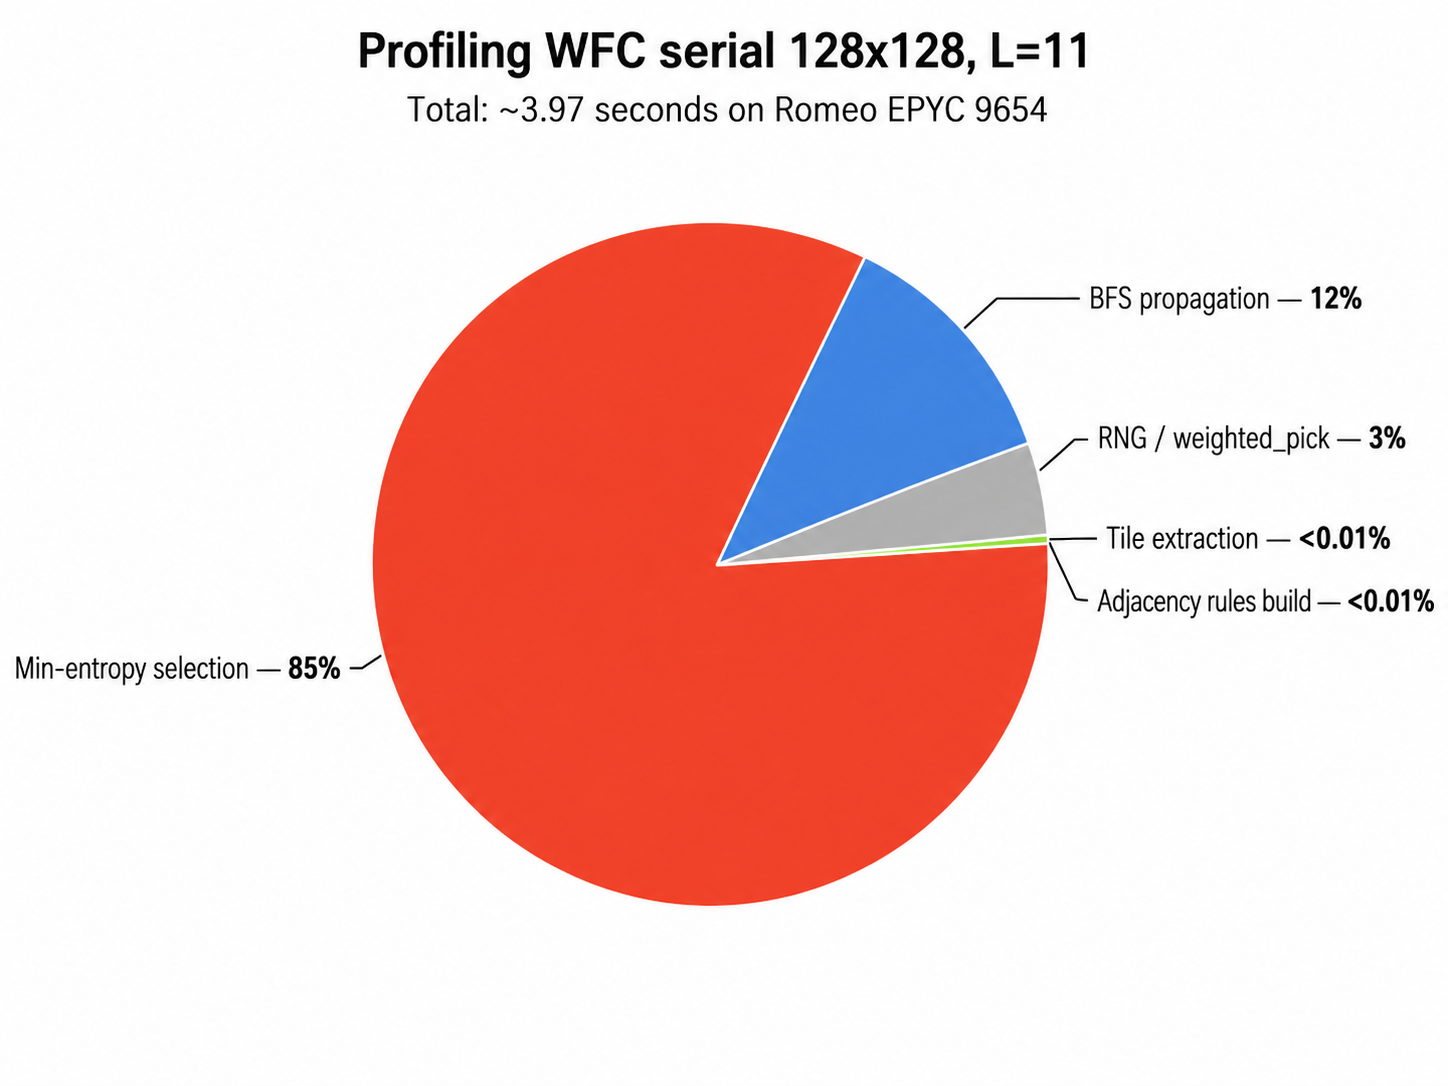
\includegraphics[width=0.7\linewidth]{results/figures/schemas/profile_breakdown.png}
\caption{Décomposition du temps sur 128×128 binaire. La sélection min-entropie domine.}
\label{fig:profile_breakdown}
\end{figure}

\subsection{Temps absolus de référence}

\begin{table}[H]
\centering
\begin{tabular}{lrr}
\toprule
\textbf{Taille} & \textbf{Solve serial (s)} & \textbf{Throughput (Mcells/s)} \\
\midrule
32×32 & 0.015 & 68 \\
64×64 & 0.247 & 16.6 \\
128×128 & 3.97 & 4.13 \\
256×256 & 61.4 & 1.07 \\
\bottomrule
\end{tabular}
\caption{Performance séquentielle sur Romeo, sample binary\_L11. Le throughput chute avec la taille à cause des cache misses (la wave déborde de la L2 à 256×256).}
\label{tab:res:serial}
\end{table}

% =============================================================================
\section{Scaling OpenMP : strong scaling}
\label{sec:res:omp_scaling}
% =============================================================================

\subsection{Speedup binary\_L11 sur Romeo}

La courbe de speedup (Fig.~\ref{fig:speedup_binary}) trace $S(p)$ pour les quatre tailles testées. Toutes les courbes montent jusqu'à un peak situé entre 4 et 16 threads selon la taille, puis chutent : à 256$\times$256, peak 8.23$\times$ à 16 threads ; à 32$\times$32, on n'atteint jamais 1.2$\times$. La forme générale est bien celle prédite par Amdahl complétée par des coûts \emph{supra}-Amdahl (fork/join, contention, frontières BFS) qui dominent au-delà du peak.

\begin{figure}[H]
\centering

\includegraphics[width=0.85\linewidth]{results/figures/scaling/speedup_binary_L11.png}
\caption{Speedup binary\_L11. Plus la grille est grande, plus le peak est élevé et plus il se déplace vers la droite.}
\label{fig:speedup_binary}
\end{figure}

La bande min/max (Fig.~\ref{fig:speedup_band_binary}) quantifie la variance entre les 3 répétitions de chaque configuration. Lecture pratique : entre 1 et 8 threads, la bande est étroite (régime stable, mesures reproductibles) ; au-delà de 32 threads, la bande s'élargit fortement, les régressions exactes varient d'un run à l'autre.

\begin{figure}[H]
\centering

\includegraphics[width=0.85\linewidth]{results/figures/scaling/speedup_band_binary_L11.png}
\caption{Bande min/max binary\_L11 (3 répétitions). Étroite en régime stable (1-8 threads), large au-delà de 32 threads.}
\label{fig:speedup_band_binary}
\end{figure}

L'efficacité parallèle $E(p) = S(p)/p$ (Fig.~\ref{fig:efficiency_binary}) donne une lecture normalisée : à 16 threads sur 256$\times$256 nous sommes à $E = 0.51$ (51\% d'efficacité) ; au-delà de 32 threads, $E$ chute sous 0.1 sur toutes les tailles. Cela quantifie un point important : ce n'est pas un \emph{plateau}, c'est un \emph{décrochage} brutal causé par la barrière par niveau BFS.

\begin{figure}[H]
\centering

\includegraphics[width=0.85\linewidth]{results/figures/scaling/efficiency_binary_L11.png}
\caption{Efficacité parallèle binary\_L11. Décrochage net au-delà de 32 threads, pas un plateau.}
\label{fig:efficiency_binary}
\end{figure}

Le throughput (Fig.~\ref{fig:throughput_binary}) inverse la lecture : à taille fixée, l'amortissement parallèle paie quand la grille est grande. Le pic à 15.4 Mcells/s sur 256$\times$256, 16 threads, est $14\times$ supérieur au serial sur la même taille (1.07 Mcells/s, Tab.~\ref{tab:res:serial}). Cela vient en partie du parallélisme et en partie du masquage des latences mémoire (la wave 524 KB déborde de la L2, le parallélisme aide à amortir les latences).

\begin{figure}[H]
\centering
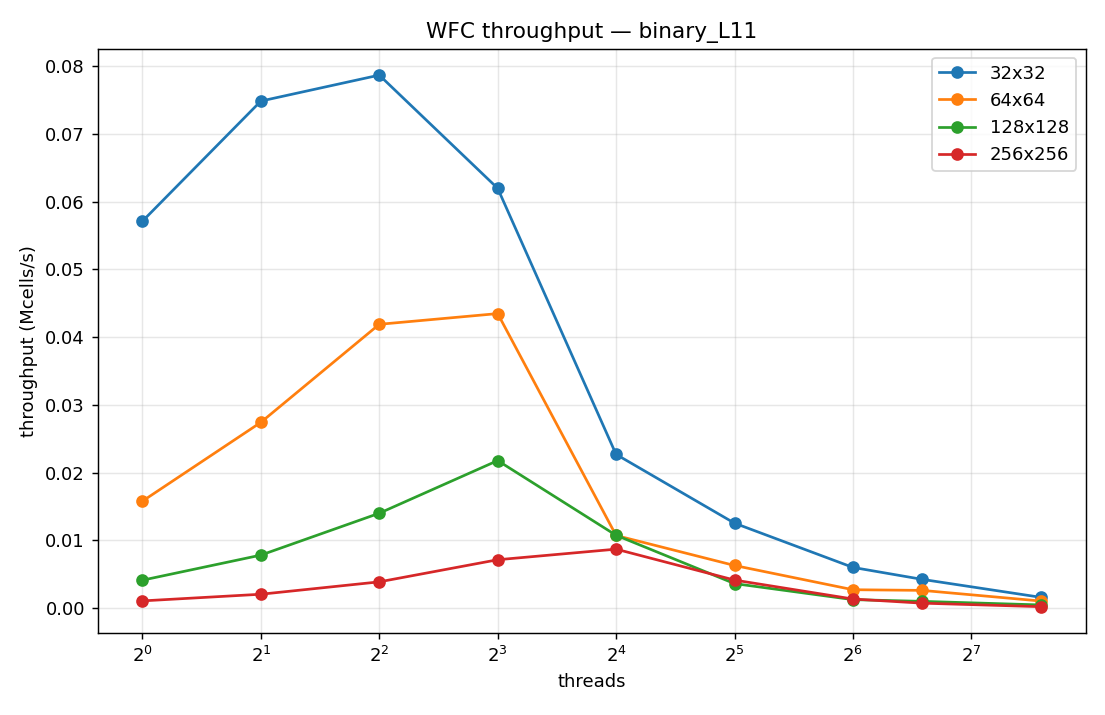
\includegraphics[width=0.85\linewidth]{results/figures/scaling/throughput_binary_L11.png}
\caption{Throughput binary\_L11. Pic 15.4 Mcells/s à 16 threads sur 256$\times$256 ($14\times$ vs serial).}
\label{fig:throughput_binary}
\end{figure}

Le heatmap taille$\times$threads (Fig.~\ref{fig:heatmap_binary}) résume le tout en deux dimensions : la \emph{diagonale} verte (sweet spot) montre que la taille optimale de grille \emph{suit} le nombre de threads. Lecture directe : à 8 threads, optimum vers 128$\times$128 ; à 16 threads, optimum vers 256$\times$256 ; à 32+ threads, le sweet spot sort de la zone mesurée (les runs 512$\times$512 ont timeout à 4h sur Romeo).

\begin{figure}[H]
\centering

\includegraphics[width=0.85\linewidth]{results/figures/scaling/heatmap_binary_L11.png}
\caption{Heatmap binary\_L11 (taille $\times$ threads, couleur = temps). Le sweet spot diagonal indique que la taille optimale suit le nombre de threads.}
\label{fig:heatmap_binary}
\end{figure}

\begin{table}[H]
\centering
\begin{tabular}{lrrrrrrrr}
\toprule
\textbf{Taille} & \textbf{1t} & \textbf{2t} & \textbf{4t} & \textbf{8t} & \textbf{16t} & \textbf{32t} & \textbf{64t} & \textbf{192t} \\
\midrule
32×32 & 1.00× & 1.10× & 1.16× & 0.91× & 0.33× & 0.18× & 0.09× & 0.02× \\
64×64 & 0.96× & 1.66× & 2.54× & 2.64× & 0.65× & 0.38× & 0.16× & 0.06× \\
128×128 & 1.00× & 1.89× & 3.39× & 5.27× & 2.60× & 0.87× & 0.30× & 0.11× \\
\textbf{256×256} & \textbf{1.00×} & \textbf{1.93×} & \textbf{3.65×} & \textbf{6.73×} & \textbf{8.23×} & \textbf{3.91×} & \textbf{1.26×} & \textbf{0.19×} \\
\bottomrule
\end{tabular}
\caption{Strong scaling binary\_L11 sur Romeo (job 543692). Peak 8.23× à 16 threads sur 256×256. Régression brutale au-delà du peak.}
\label{tab:res:speedup_binary}
\end{table}

\begin{important}{Lecture du tableau}
\begin{itemize}
    \item À 32×32, le parallélisme ne paie jamais : la grille est trop petite pour amortir le coût des tasks.
    \item À 64×64, peak modeste à 4-8 threads ; au-delà, régression rapide.
    \item À 128×128, peak 5.27× à 8 threads, déjà honorable.
    \item À 256×256, peak 8.23× à 16 threads (51\% d'efficacité parallèle). C'est notre meilleur résultat.
    \item Au-delà du peak (32+ threads), régression brutale jusqu'à 0.02× la baseline à 192 threads sur 32×32 (le solver tourne 50× plus lentement que le serial).
\end{itemize}
\end{important}

\subsection{Causes de la régression à haut nombre de threads}

Trois causes dominent :

\begin{enumerate}
    \item \textbf{Frontière BFS trop courte} : un niveau de 10 cellules sur 192 threads → 18 threads sur 19 attendent à la barrière. Le coût synchronisation domine.

    \item \textbf{Fork/join répété} : la barrière par niveau coûte $\sim 50$ µs sur 192 cores. Pour 8000 niveaux : 400 ms incompressibles, à comparer aux $\sim 100$ ms de travail utile.

    \item \textbf{Contention atomique inter-NUMA} : \texttt{\_\_atomic\_fetch\_and} cross-NUMA = ping-pong de cache lines à 1-3 µs par opération.
\end{enumerate}

L'optim « frontier-threshold » (Section~\ref{sec:res:optim_frontier}) atténue (1) et (2) mais pas (3).

% =============================================================================
\section{Modèle d'Amdahl}
\label{sec:res:amdahl}
% =============================================================================

Pour caractériser le scaling, nous fittons Amdahl $S(p) = 1 / ((1-f) + f/p)$ par moindres carrés non-linéaires sur la portion croissante de chaque courbe (avant le décrochage). Le fit retourne $f$ (fraction parallélisable) et le ceiling théorique $S_\infty = 1/(1-f)$. Les courbes sont en échelle log-log avec la droite « idéale » $S = p$ pour repère.

\subsection{Évolution du fit avec la taille de grille}

La mosaïque (Fig.~\ref{fig:amdahl_binary_grid}) trace les 4 fits binary\_L11 pour les 4 tailles testées. La fraction parallélisable $f$ croît brutalement avec la taille : 0.18 (32$\times$32) $\to$ 0.74 (64$\times$64) $\to$ 0.93 (128$\times$128) $\to$ 0.94 (256$\times$256). Lecture algorithmique : les coûts fixes (extraction tuiles, init wave, fork/join initial) deviennent rapidement négligeables face au travail utile dès que la grille dépasse 64$\times$64.

\begin{figure}[H]
\centering
\begin{subfigure}[t]{0.48\linewidth}
\centering
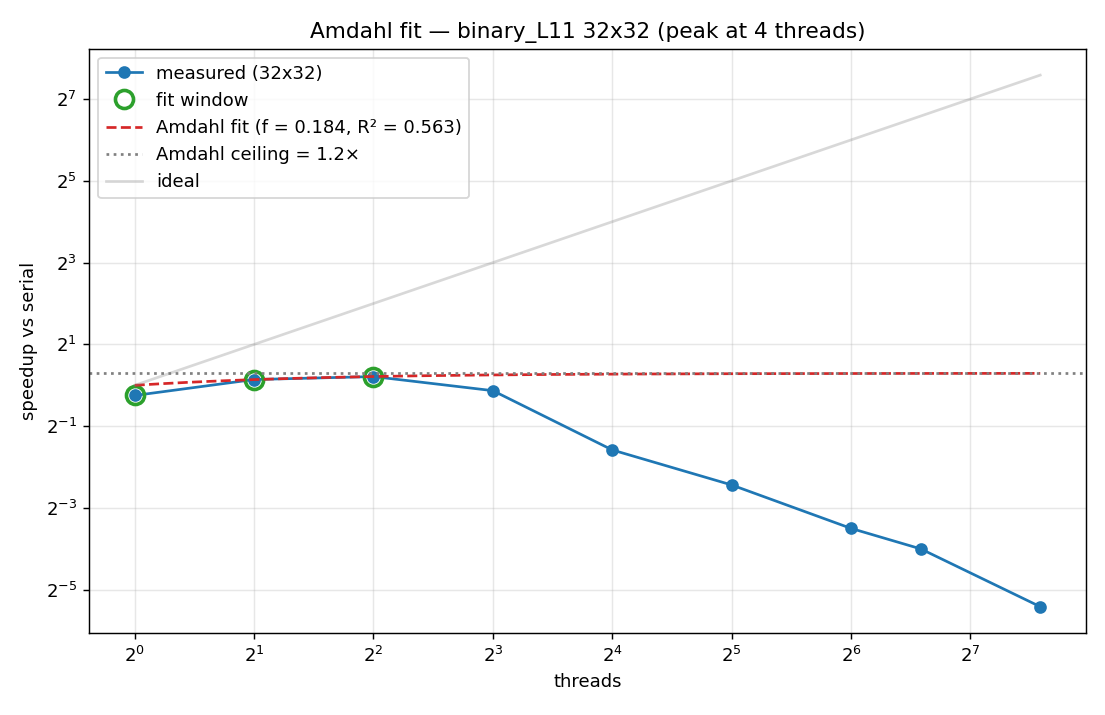
\includegraphics[width=\linewidth]{results/figures/amdahl/amdahl_binary_L11_32.png}
\caption{32×32, $f = 0.18$, ceiling $1.2\times$.}
\end{subfigure}\hfill
\begin{subfigure}[t]{0.48\linewidth}
\centering
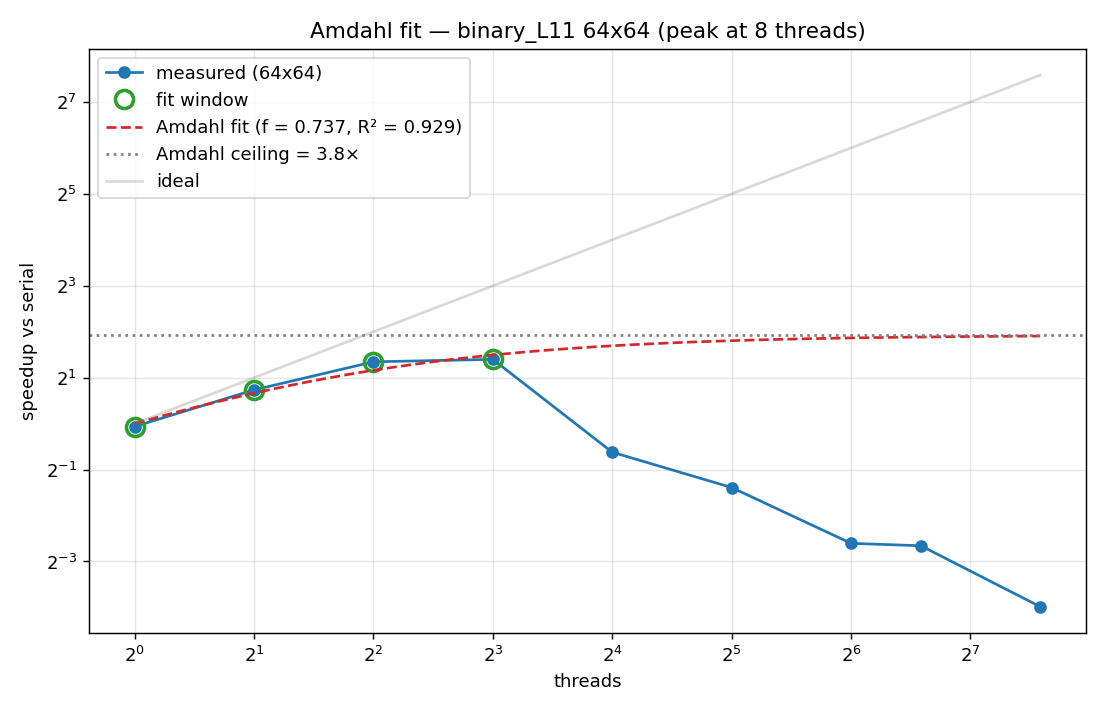
\includegraphics[width=\linewidth]{results/figures/amdahl/amdahl_binary_L11_64.png}
\caption{64×64, $f = 0.74$, ceiling $3.8\times$.}
\end{subfigure}

\vspace{0.5em}

\begin{subfigure}[t]{0.48\linewidth}
\centering
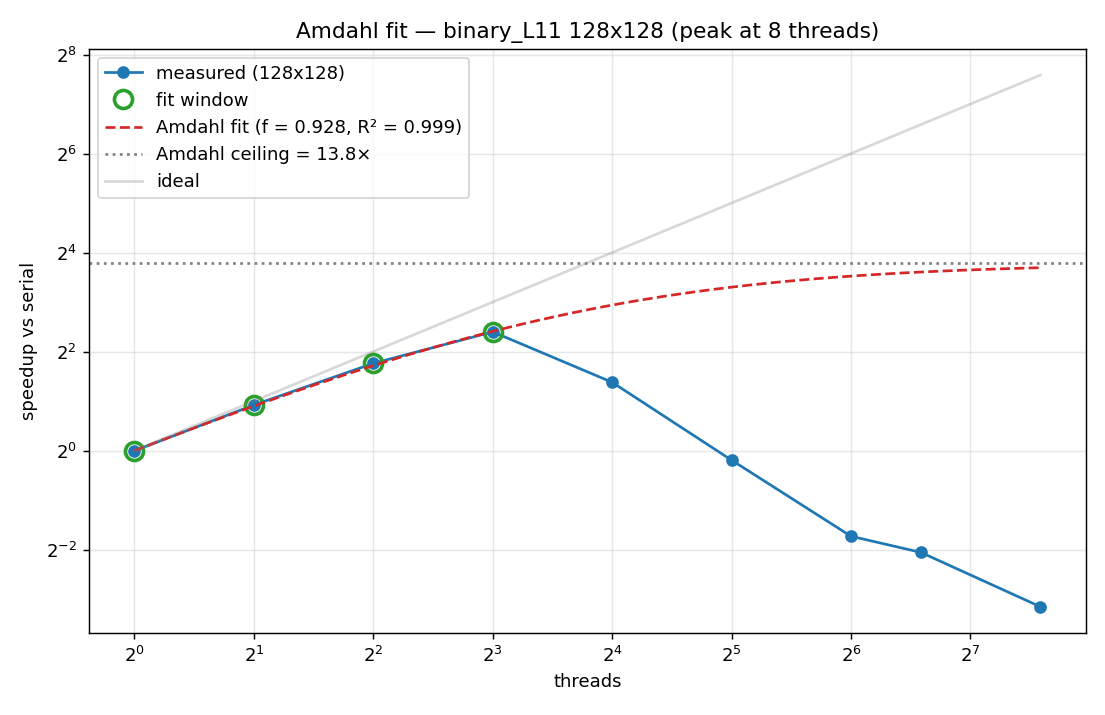
\includegraphics[width=\linewidth]{results/figures/amdahl/amdahl_binary_L11_128.png}
\caption{128×128, $f = 0.93$, ceiling $13.8\times$.}
\end{subfigure}\hfill
\begin{subfigure}[t]{0.48\linewidth}
\centering
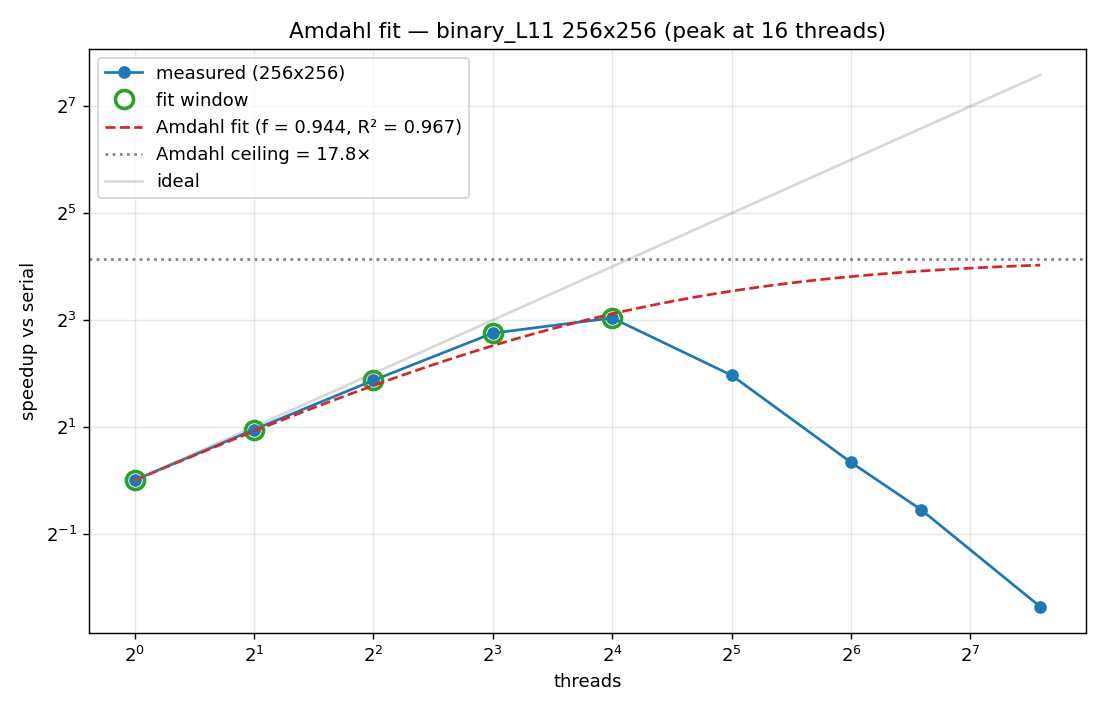
\includegraphics[width=\linewidth]{results/figures/amdahl/amdahl_binary_L11_256.png}
\caption{256×256, $f = 0.94$, ceiling $17.8\times$.}
\end{subfigure}

\caption[Évolution du fit Amdahl binary\_L11 par taille.]{Évolution
du fit Amdahl binary\_L11 avec la taille de grille. La fraction
parallélisable $f$ croît rapidement de 0.18 (32×32) à 0.94 (256×256) :
plus la grille est grande, plus propagation et sélection min-entropie
dominent face aux coûts fixes.}
\label{fig:amdahl_binary_grid}
\end{figure}

\subsection{Effet de l'optim « frontier-threshold » sur Amdahl}

Re-fitter Amdahl après activation de l'optim frontier-threshold (Fig.~\ref{fig:amdahl_binary_optim}) déplace les paramètres du modèle : $f$ passe de 0.928 à 0.956, le ceiling théorique de $13.8\times$ à $22.9\times$. Le peak observé monte de $5.27\times$ à $6.10\times$ : l'optim ne ferme pas l'écart au ceiling (les coûts supra-Amdahl restent), mais elle pousse le mur plus loin.

\begin{figure}[H]
\centering
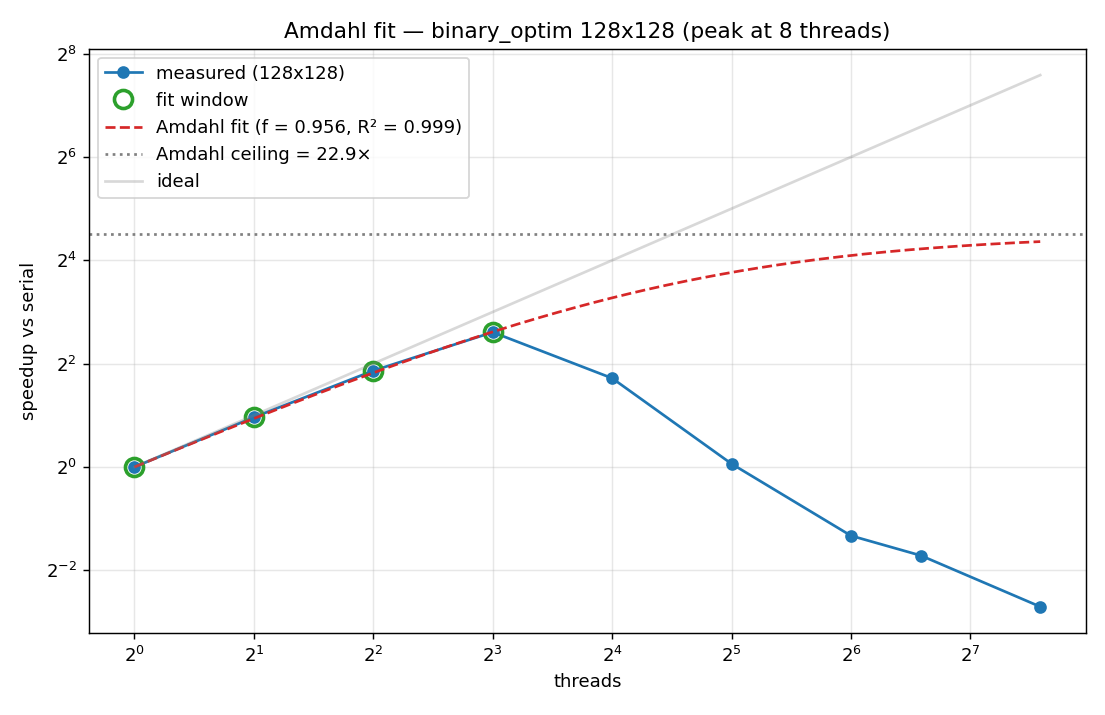
\includegraphics[width=0.85\linewidth]{results/figures/amdahl/amdahl_binary_optim_128.png}
\caption[Fit Amdahl binary 128 après optim frontier-threshold.]{Fit
Amdahl binary\_L11 128×128 après frontier-threshold. $f$ passe de
0.928 à 0.956, ceiling de $13.8\times$ à $22.9\times$.}
\label{fig:amdahl_binary_optim}
\end{figure}

\subsection{Amdahl sur autres samples}

La mosaïque par sample (Fig.~\ref{fig:amdahl_other_samples}) compare terrain\_L33 et smooth\_N3 sur 3 tailles. terrain\_L33 suit le même pattern que binary\_L11 (croissance régulière de $f$ avec la taille). smooth\_N3 plafonne à $f = 0.74$ même à 128$\times$128 : peu de tuiles ($L=12$) combiné à $N=3$ produit des frontières BFS courtes qui propagent peu, donc peu de parallélisme exploitable. C'est une limite \emph{structurelle} du sample, pas une marge d'optimisation.

\begin{figure}[H]
\centering
\begin{subfigure}[t]{0.31\linewidth}
\centering
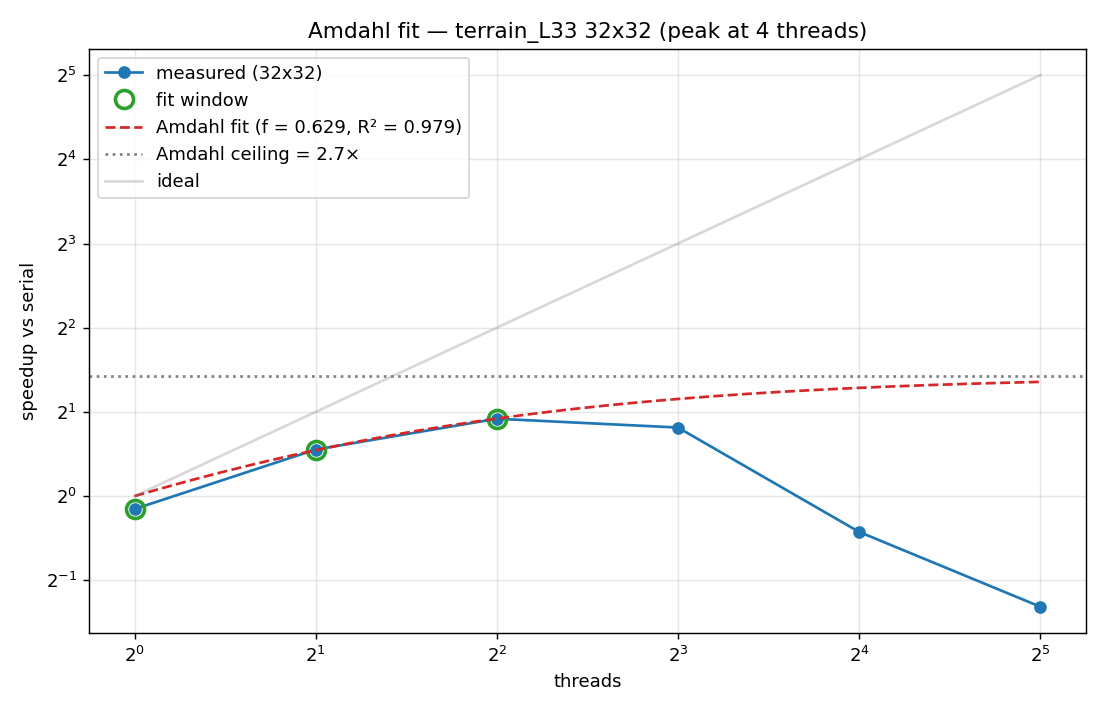
\includegraphics[width=\linewidth]{results/figures/amdahl/amdahl_terrain_L33_32.png}
\caption{terrain 32×32.}
\end{subfigure}\hfill
\begin{subfigure}[t]{0.31\linewidth}
\centering
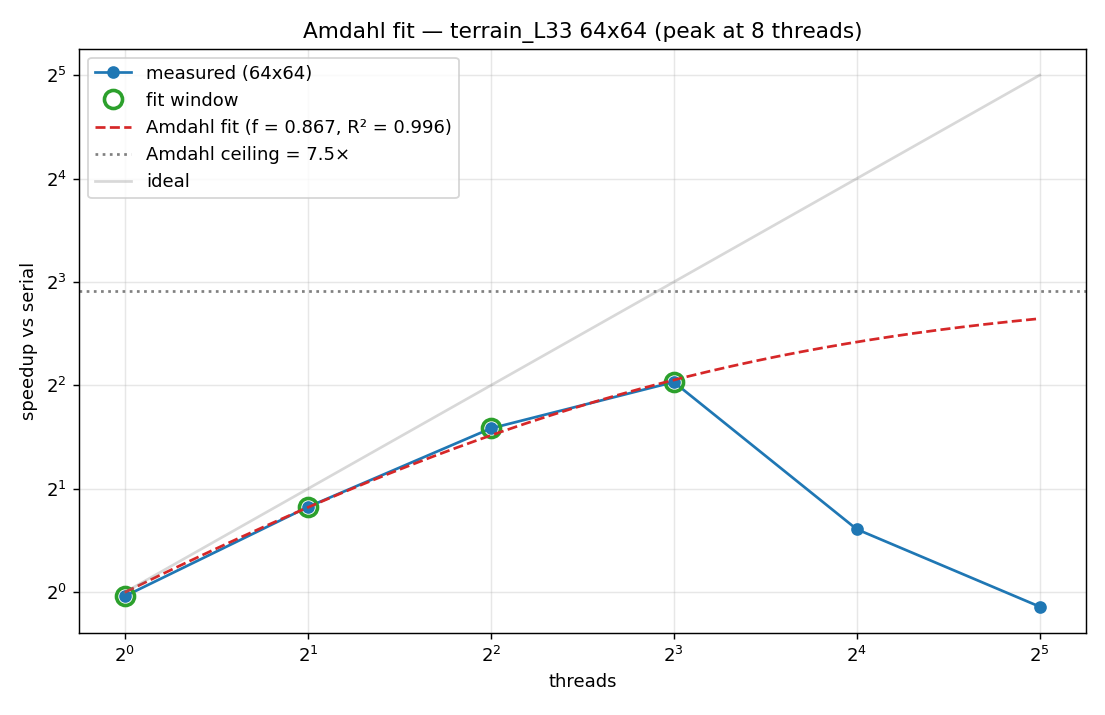
\includegraphics[width=\linewidth]{results/figures/amdahl/amdahl_terrain_L33_64.png}
\caption{terrain 64×64.}
\end{subfigure}\hfill
\begin{subfigure}[t]{0.31\linewidth}
\centering
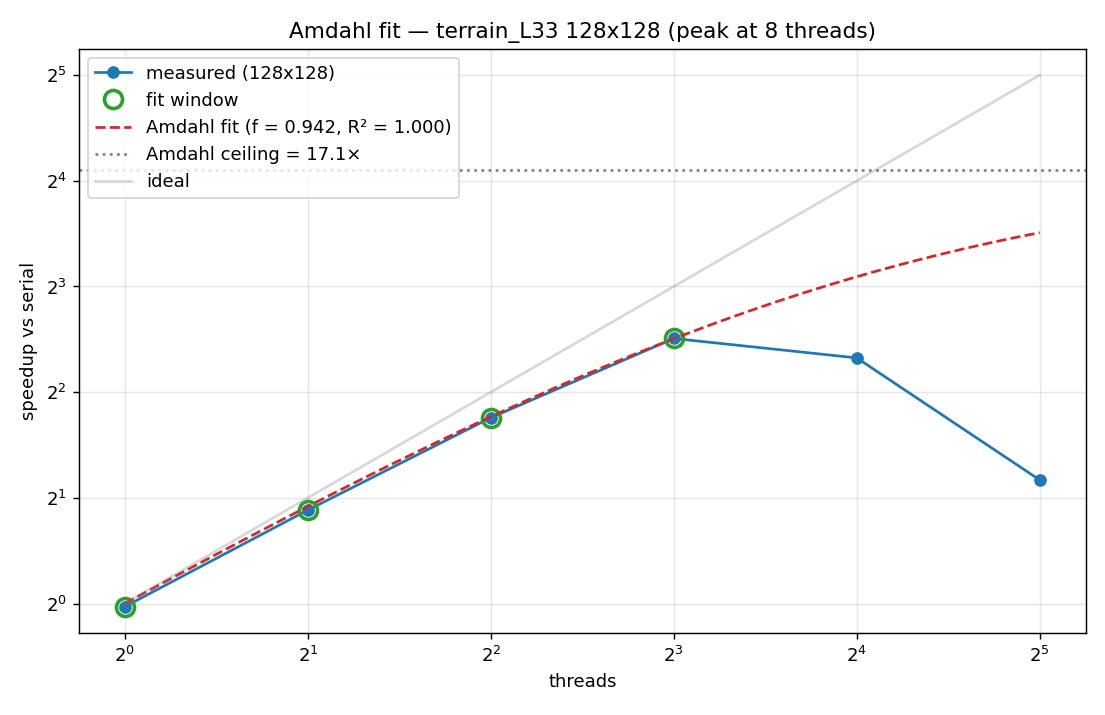
\includegraphics[width=\linewidth]{results/figures/amdahl/amdahl_terrain_L33_128.png}
\caption{terrain 128×128, $f=0.94$.}
\end{subfigure}

\vspace{0.5em}

\begin{subfigure}[t]{0.31\linewidth}
\centering
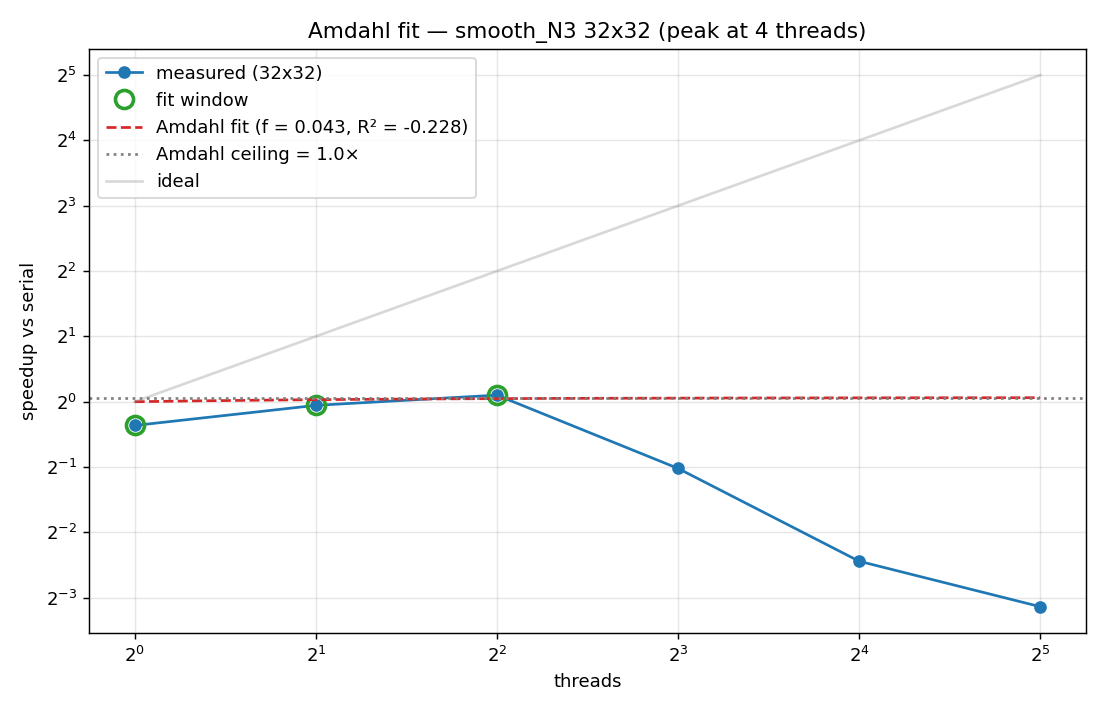
\includegraphics[width=\linewidth]{results/figures/amdahl/amdahl_smooth_N3_32.png}
\caption{smooth\_N3 32×32.}
\end{subfigure}\hfill
\begin{subfigure}[t]{0.31\linewidth}
\centering
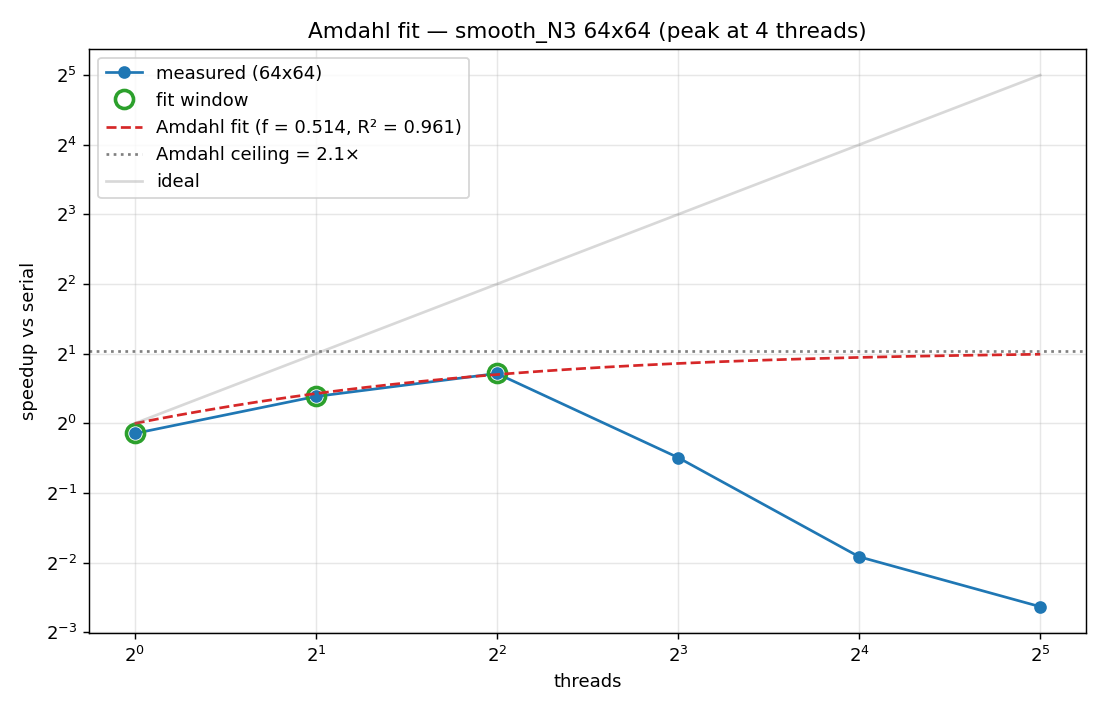
\includegraphics[width=\linewidth]{results/figures/amdahl/amdahl_smooth_N3_64.png}
\caption{smooth\_N3 64×64.}
\end{subfigure}\hfill
\begin{subfigure}[t]{0.31\linewidth}
\centering
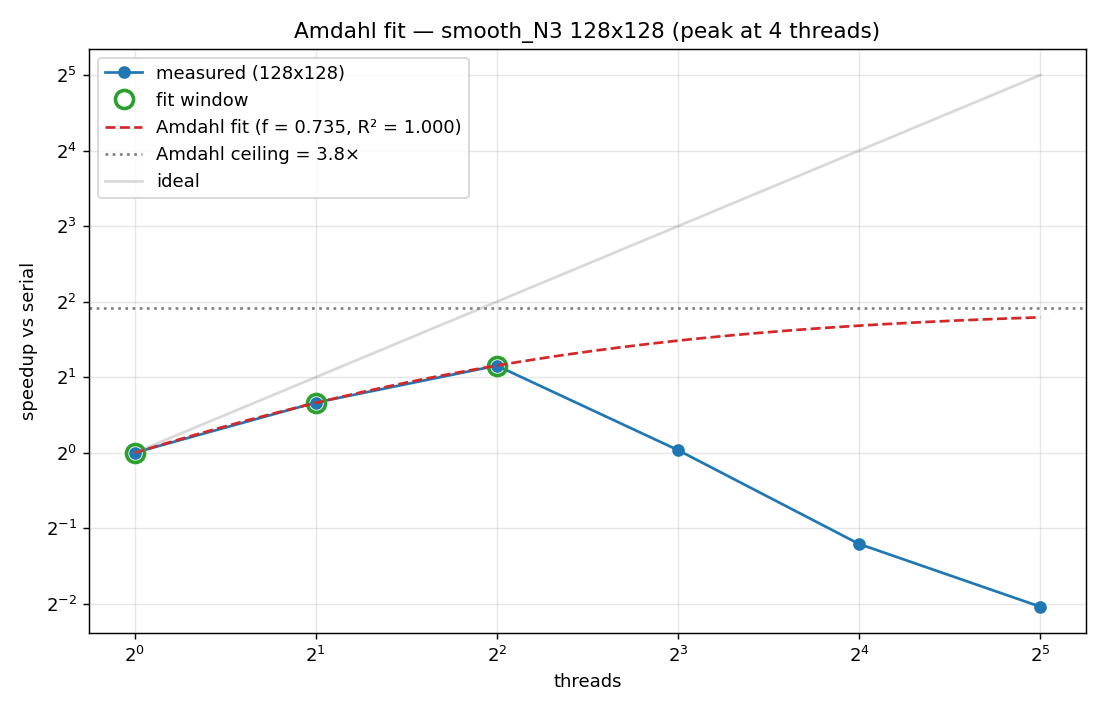
\includegraphics[width=\linewidth]{results/figures/amdahl/amdahl_smooth_N3_128.png}
\caption{smooth\_N3 128×128, $f=0.74$.}
\end{subfigure}

\caption[Fits Amdahl par sample : terrain et smooth.]{Fits Amdahl
par sample × taille. terrain\_L33 suit le même pattern que
binary\_L11 (croissance de $f$ avec la taille). smooth\_N3 plafonne à
$f = 0.74$ même à 128×128 : peu de tuiles ($L=12$) et $N=3$ $\to$
parallélisme structurel limité, indépendamment de la grille.}
\label{fig:amdahl_other_samples}
\end{figure}

\begin{table}[H]
\centering
\begin{tabular}{llrrrrr}
\toprule
\textbf{Label} & \textbf{Size} & \textbf{$f$} & \textbf{$R^2$} & \textbf{Ceiling} & \textbf{Peak} & \textbf{Ratio} \\
\midrule
binary\_L11 & 32 & 0.184 & 0.563 & 1.2× & 1.16× & 95\% \\
binary\_L11 & 64 & 0.737 & 0.929 & 3.8× & 2.64× & 69\% \\
binary\_L11 & 128 & 0.928 & 0.999 & 13.8× & 5.27× & 38\% \\
binary\_L11 & 256 & 0.944 & 0.967 & 17.8× & 8.23× & 46\% \\
binary\_optim & 128 & 0.956 & 0.999 & 22.9× & 6.10× & 27\% \\
terrain\_L33 & 64 & 0.867 & 0.996 & 7.5× & 4.09× & 54\% \\
terrain\_L33 & 128 & 0.942 & 1.000 & 17.1× & 5.69× & 33\% \\
smooth\_N3 & 128 & 0.735 & 1.000 & 3.8× & 2.23× & 59\% \\
\bottomrule
\end{tabular}
\caption{Fits Amdahl par configuration. À 128 et 256, $f \approx 0.94$ pour binary et terrain : le code est ~94\% parallélisable, ceiling théorique 14-18×. Le peak observé reste à 33-46\% du ceiling : Amdahl suppose un parallélisme parfait, la réalité inclut des coûts supra-linéaires.}
\label{tab:res:amdahl}
\end{table}

\begin{important}{Lecture du fit Amdahl}
\begin{itemize}
    \item L'optim « frontier-threshold » pousse $f$ de 0.928 à 0.956 sur 128×128 (peak 5.27× → 6.10×, ceiling théorique 13.8 → 22.9).
    \item Le ratio peak/ceiling baisse, mais le peak absolu monte. L'optim aide.
    \item \texttt{smooth\_N3} a $f = 0.735$ au max, beaucoup moins parallélisable. Cause : peu de tuiles ($L=12$) + $N=3$ = peu de parallélisme par cellule (analyse en Section~\ref{sec:res:varying_datasets}).
\end{itemize}
\end{important}

% =============================================================================
\section{Varying datasets : impact du sample}
\label{sec:res:varying_datasets}
% =============================================================================

À taille de grille fixée (128×128) et thread count variable, le sample modifie significativement le scaling.

\subsection{terrain\_L33 vs binary\_L11}

terrain\_L33 (33 tuiles, $N=2$) scale mieux que binary\_L11 à taille égale. Sur 128$\times$128 (Fig.~\ref{fig:speedup_terrain}), le peak est 5.69$\times$ à 8 threads contre 5.27$\times$ pour binary\_L11. La différence vient du travail par cellule : 33 bits à manipuler par cellule vs 11, donc plus d'opérations utiles à amortir, et l'overhead OMP relatif diminue.

\begin{figure}[H]
\centering
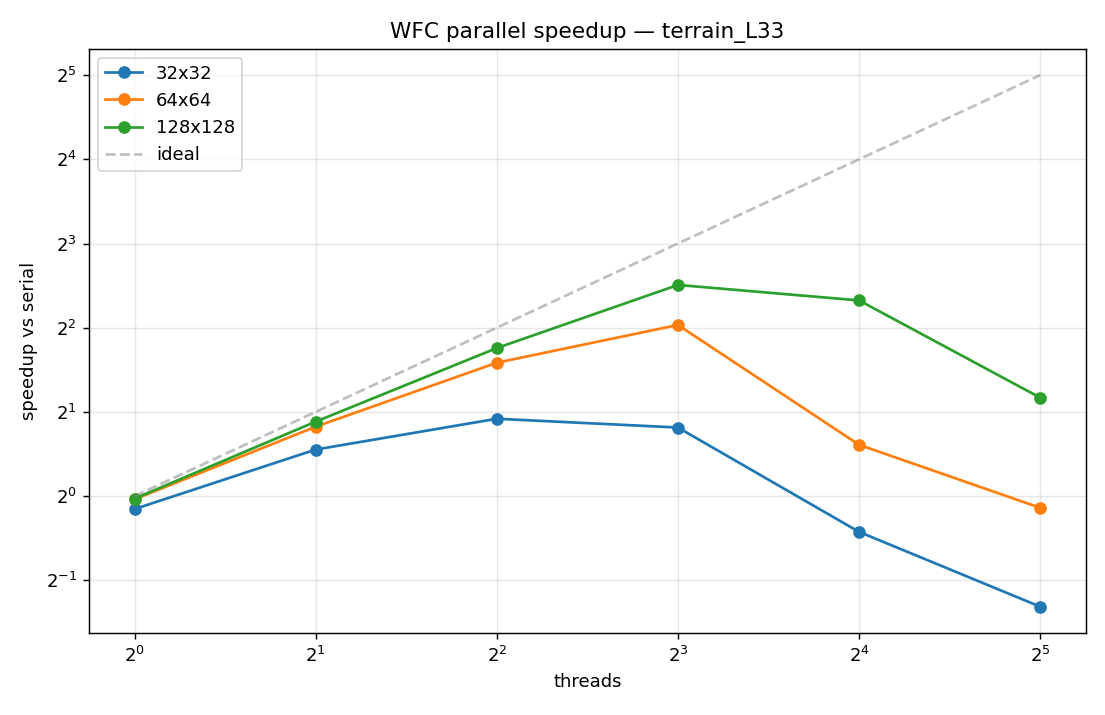
\includegraphics[width=0.85\linewidth]{results/figures/scaling/speedup_terrain_L33.png}
\caption{Speedup terrain\_L33. Peak 5.69$\times$ à 8 threads sur 128$\times$128.}
\label{fig:speedup_terrain}
\end{figure}

L'efficacité et le throughput (Fig.~\ref{fig:scaling_terrain_combo}) confirment : à 8 threads sur 128$\times$128, $E \approx 0.71$ (71\% d'efficacité, vs 65\% pour binary à la même configuration). Le décrochage post-peak est aussi moins brutal, la bande min/max (Fig.~\ref{fig:speedup_band_terrain}) reste étroite jusqu'à 16 threads.

\begin{figure}[H]
\centering
\begin{subfigure}[t]{0.48\linewidth}
\centering
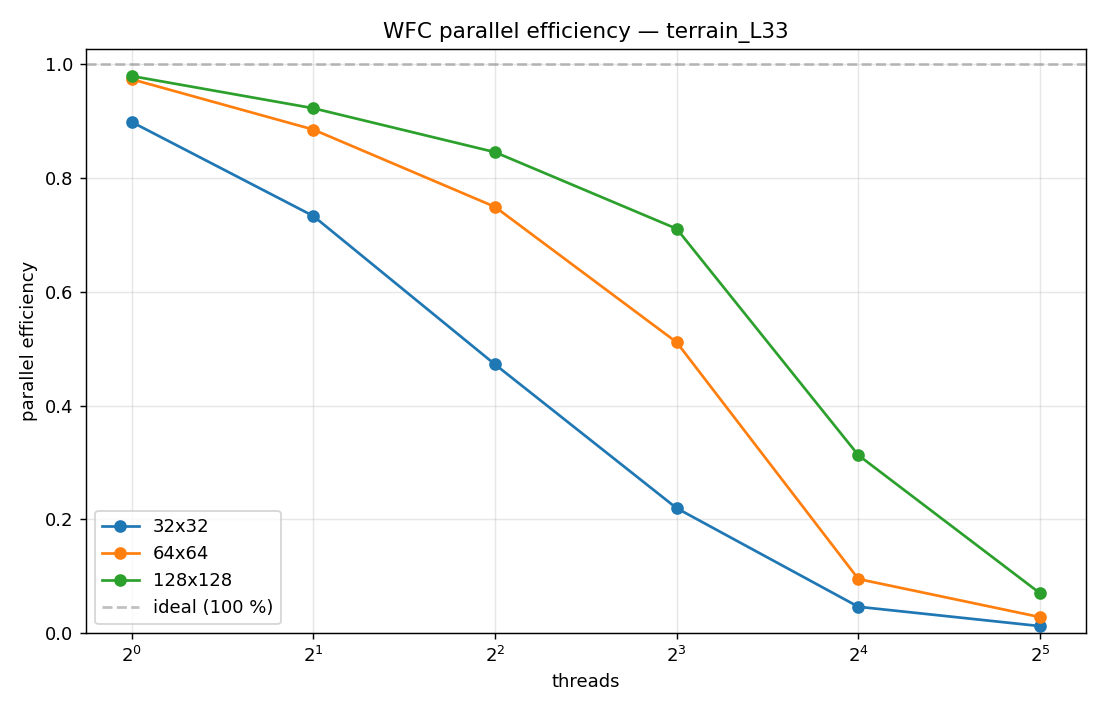
\includegraphics[width=\linewidth]{results/figures/scaling/efficiency_terrain_L33.png}
\caption{Efficacité parallèle terrain\_L33.}
\end{subfigure}\hfill
\begin{subfigure}[t]{0.48\linewidth}
\centering
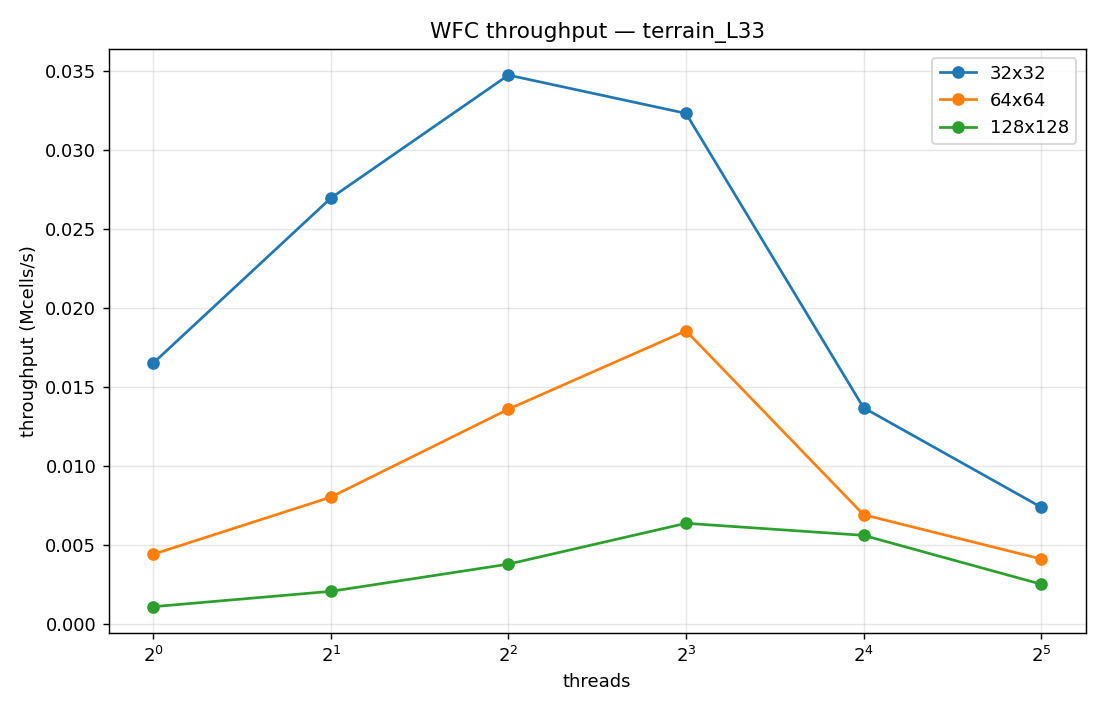
\includegraphics[width=\linewidth]{results/figures/scaling/throughput_terrain_L33.png}
\caption{Throughput terrain\_L33.}
\end{subfigure}

\caption{terrain\_L33 efficacité + throughput. À 128$\times$128 et 8 threads, $E \approx 0.71$ (vs 0.65 pour binary\_L11).}
\label{fig:scaling_terrain_combo}
\end{figure}

Le heatmap terrain\_L33 (Fig.~\ref{fig:heatmap_terrain}) montre un sweet spot diagonal plus large que pour binary\_L11 : la plage de configurations exploitables est plus tolérante au choix taille$\times$threads.

\begin{figure}[H]
\centering
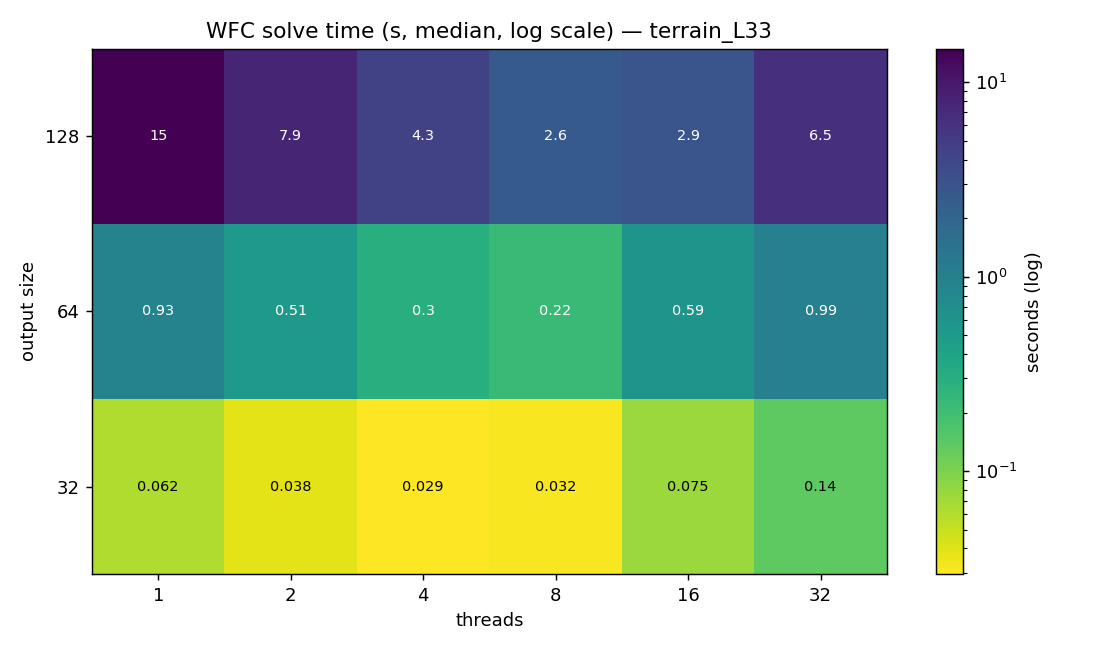
\includegraphics[width=0.85\linewidth]{results/figures/scaling/heatmap_terrain_L33.png}
\caption{Heatmap terrain\_L33. Sweet spot diagonal plus large que binary\_L11.}
\label{fig:heatmap_terrain}
\end{figure}

\begin{figure}[H]
\centering
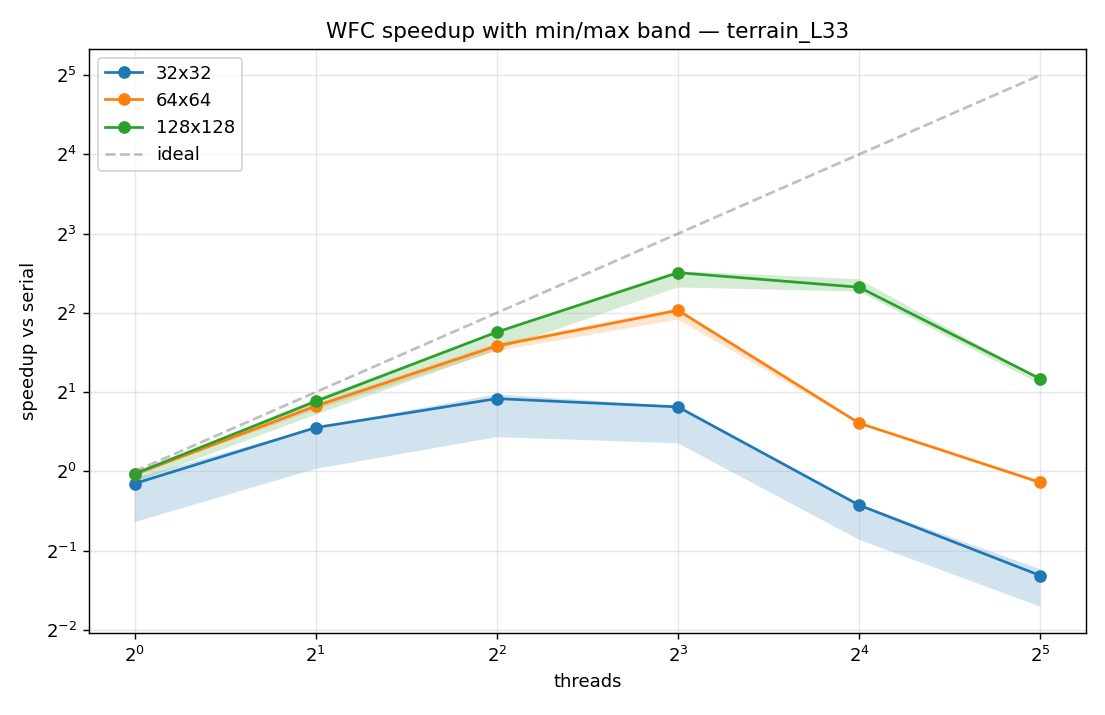
\includegraphics[width=0.85\linewidth]{results/figures/scaling/speedup_band_terrain_L33.png}
\caption{Bande min/max terrain\_L33. Étroite jusqu'à 16 threads.}
\label{fig:speedup_band_terrain}
\end{figure}

\begin{table}[H]
\centering
\begin{tabular}{lrrrrrr}
\toprule
\textbf{Sample} & \textbf{$L$} & \textbf{1t} & \textbf{4t} & \textbf{8t} & \textbf{16t} & \textbf{32t} \\
\midrule
binary\_L11 128×128 & 11 & 1.00× & 3.39× & 5.27× & 2.60× & 0.87× \\
terrain\_L33 128×128 & 33 & 1.00× & 3.43× & \textbf{5.69×} & 4.81× & 2.13× \\
\bottomrule
\end{tabular}
\caption{terrain\_L33 (33 tuiles) atteint un meilleur peak que binary\_L11 (11 tuiles) à taille égale. La différence vient du travail par cellule : plus de bits → meilleur amortissement OMP.}
\label{tab:res:terrain_vs_binary}
\end{table}

\subsection{smooth\_N3, le cas pathologique}

smooth\_N3 (12 tuiles, $N=3$, gradients lisses) plafonne à 2.23$\times$ à 4 threads sur 128$\times$128 (Fig.~\ref{fig:speedup_smooth}) et régresse dès 8 threads. Cause : les motifs lisses produisent des frontières BFS très courtes (peu de cellules touchées par niveau). Combiné à 12 tuiles seulement, le travail par niveau est insuffisant pour amortir les barrières OMP au-delà de 4 threads.

\begin{figure}[H]
\centering

\includegraphics[width=0.85\linewidth]{results/figures/scaling/speedup_smooth_N3.png}
\caption{Speedup smooth\_N3. Peak 2.23$\times$ à 4 threads, régression dès 8.}
\label{fig:speedup_smooth}
\end{figure}

L'efficacité et le throughput (Fig.~\ref{fig:scaling_smooth_combo}) confirment : plateau à 4 threads, puis décrochage. Le heatmap (Fig.~\ref{fig:heatmap_smooth}) montre un sweet spot étroit autour de 4 threads, indépendant de la taille de grille — c'est une borne \emph{structurelle} du sample, pas un paramètre à optimiser.

\begin{figure}[H]
\centering
\begin{subfigure}[t]{0.48\linewidth}
\centering

\includegraphics[width=\linewidth]{results/figures/scaling/efficiency_smooth_N3.png}
\caption{Efficacité smooth\_N3.}
\end{subfigure}\hfill
\begin{subfigure}[t]{0.48\linewidth}
\centering
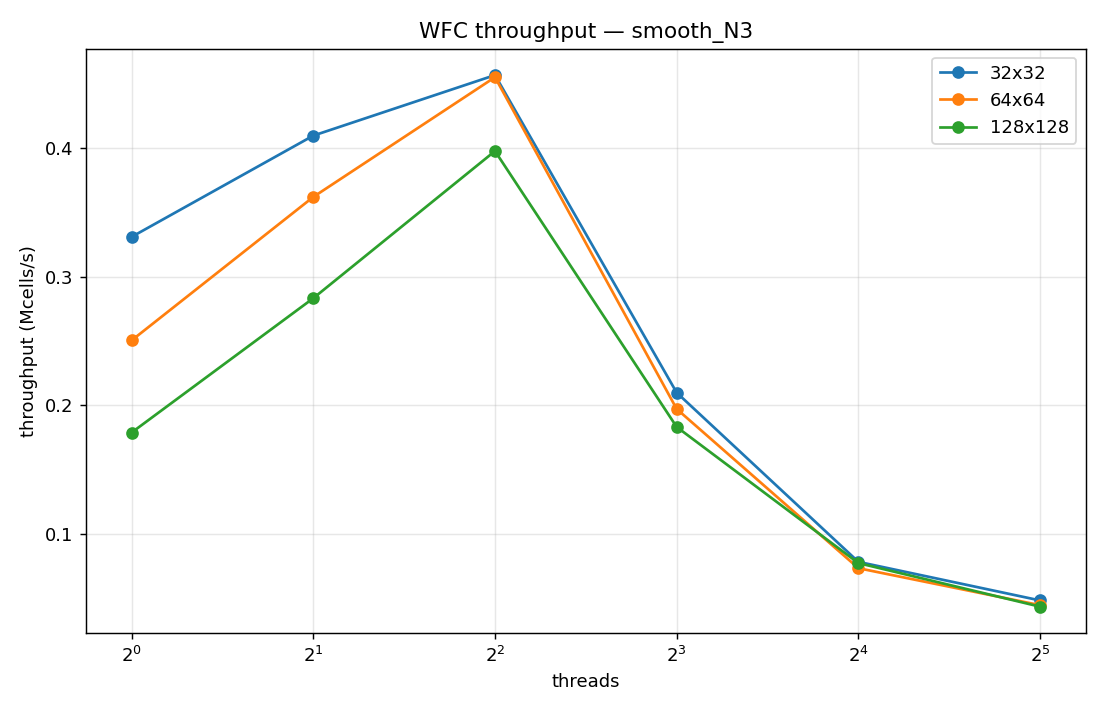
\includegraphics[width=\linewidth]{results/figures/scaling/throughput_smooth_N3.png}
\caption{Throughput smooth\_N3.}
\end{subfigure}

\caption{smooth\_N3 efficacité + throughput. Plateau à 4 threads, décrochage au-delà.}
\label{fig:scaling_smooth_combo}
\end{figure}

\begin{figure}[H]
\centering

\includegraphics[width=0.85\linewidth]{results/figures/scaling/heatmap_smooth_N3.png}
\caption{Heatmap smooth\_N3. Sweet spot étroit autour de 4 threads, indépendant de la taille.}
\label{fig:heatmap_smooth}
\end{figure}

\begin{figure}[H]
\centering

\includegraphics[width=0.85\linewidth]{results/figures/scaling/speedup_band_smooth_N3.png}
\caption{Bande min/max smooth\_N3. Élargissement dès 8 threads : variance forte hors du sweet spot.}
\label{fig:speedup_band_smooth}
\end{figure}

\begin{table}[H]
\centering
\begin{tabular}{lrrrrrr}
\toprule
\textbf{Taille} & \textbf{1t} & \textbf{2t} & \textbf{4t} & \textbf{8t} & \textbf{16t} & \textbf{32t} \\
\midrule
32×32 & 1.00× & 0.96× & 1.07× & 0.49× & 0.18× & 0.11× \\
64×64 & 1.00× & 1.50× & 1.64× & 0.71× & 0.27× & 0.16× \\
128×128 & 1.00× & 1.85× & \textbf{2.23×} & 1.16× & 0.43× & 0.24× \\
\bottomrule
\end{tabular}
\caption{smooth\_N3 plafonne à 2.23×. Cause : $L = 12$ tuiles (peu) + $N = 3$ (offsets $5 \times 5 = 25$) → 300 ops/cell, à comparer à 99 pour binary. Frontières BFS courtes car les motifs lisses propagent peu.}
\label{tab:res:smooth_N3}
\end{table}

\begin{important}{Pourquoi smooth\_N3 plafonne}
\begin{itemize}
    \item Sample de 12 tuiles seulement (gradients lisses).
    \item $N = 3$ → offsets $5 \times 5 = 25$ vs 9 pour $N = 2$. Plus d'offsets, mais peu de bits par tuile à manipuler ($L = 12$ tient dans 1 mot).
    \item Motifs lisses → propagation locale qui modifie peu de cellules par niveau.
    \item Au total, chaque niveau BFS coûte trop peu pour amortir la barrière OMP au-delà de 4 threads.
\end{itemize}

Pas de fix algorithmique côté intra-attempt sans risquer de régresser binary. Contournements utilisateur : \texttt{--threads 4} (sweet spot intra-attempt) ou \texttt{--parallel-attempts K} si retries fréquents.
\end{important}

% =============================================================================
\section{Varying configurations : impact des paramètres}
\label{sec:res:varying_configs}
% =============================================================================

\subsection{Effet de la taille de grille}

À threads fixés (16) et sample fixé (binary\_L11) :

\begin{table}[H]
\centering
\begin{tabular}{lrrrr}
\toprule
\textbf{Taille} & \textbf{Wave size} & \textbf{Cache fit} & \textbf{Speedup 16t} & \textbf{Throughput (Mcells/s)} \\
\midrule
32×32 & 8 KB & L1 ✓ & 0.33× & 4.6 \\
64×64 & 32 KB & L1 borderline & 0.65× & 11.0 \\
128×128 & 128 KB & L2 ✓ & 2.60× & 13.4 \\
256×256 & 524 KB & L2 → LLC & 8.23× & \textbf{15.4} \\
\bottomrule
\end{tabular}
\caption{À 16 threads, le speedup et throughput augmentent avec la taille jusqu'à 256×256. La wave déborde de la L2 à 256×256 ; le parallélisme aide à amortir les latences mémoire.}
\label{tab:res:varying_size}
\end{table}

\subsection{Effet du paramètre $N$}

\begin{table}[H]
\centering
\begin{tabular}{lrrrr}
\toprule
\textbf{Sample} & \textbf{$N$} & \textbf{$L$} & \textbf{Solve serial 64×64 (s)} & \textbf{Note} \\
\midrule
\texttt{binary\_5x5} & 2 & 11 & 0.247 & Référence sujet \\
\texttt{multivalue\_terrain} & 2 & 33 & 0.520 & Plus de tuiles, plus lent \\
\texttt{multivalue\_terrain} & 3 & 73 & échec & $L = 73 > $ trop contraint \\
\texttt{multivalue\_smooth} & 3 & 12 & 0.020 & Sample petit, peu de tuiles \\
\bottomrule
\end{tabular}
\caption{Impact de $N$ et du sample sur le coût serial. $N = 3$ avec terrain échoue (trop contraint), $N = 2$ avec terrain converge en ~0.5 s.}
\label{tab:res:varying_N}
\end{table}

% =============================================================================
\section{Optim « frontier-threshold » : A/B Romeo}
\label{sec:res:optim_frontier}
% =============================================================================

\begin{figure}[H]
\centering
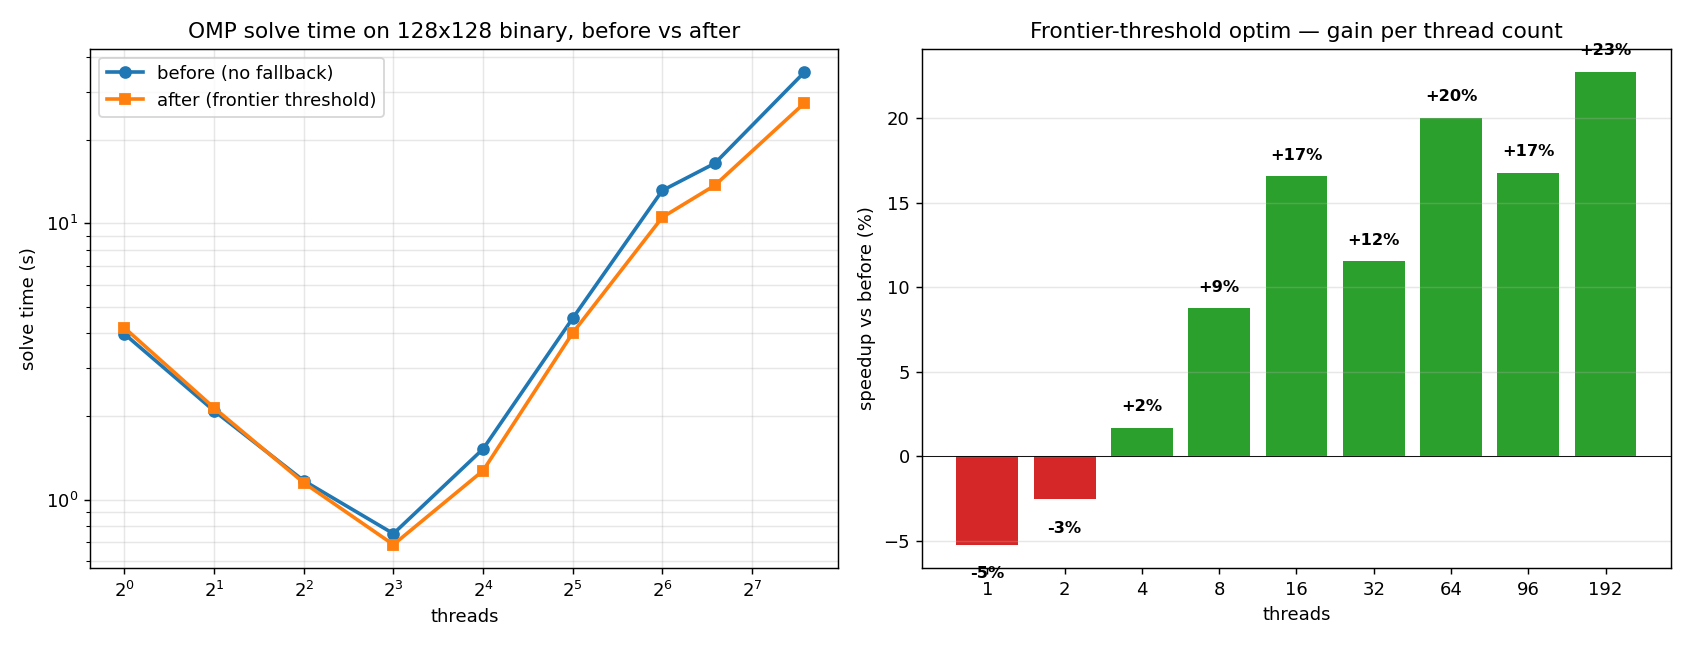
\includegraphics[width=0.85\linewidth]{results/figures/optim/frontier_threshold_compare.png}
\caption{A/B « frontier-threshold » sur binary\_L11 128×128 (job 544356).}
\label{fig:optim_frontier}
\end{figure}

\subsection{Profil de scaling complet \emph{après} optim (binary\_optim)}

Le run \texttt{binary\_optim} re-mesure binary\_L11 128×128 avec
\texttt{frontier-threshold} activé. On observe ainsi non pas un seul
nombre (gain à un thread count) mais l'évolution complète du
speedup, de l'efficacité et du throughput sous le régime optimisé.

\begin{figure}[H]
\centering
\begin{subfigure}[t]{0.48\linewidth}
\centering
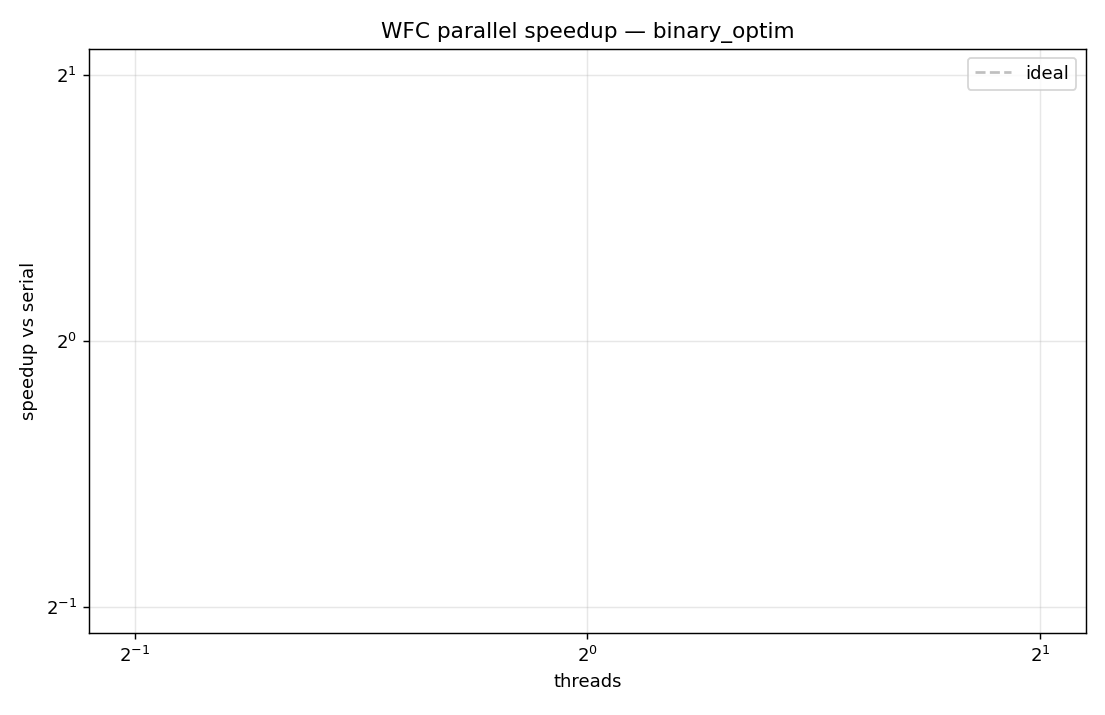
\includegraphics[width=\linewidth]{results/figures/scaling/speedup_binary_optim.png}
\caption{Speedup binary\_optim 128.}
\end{subfigure}\hfill
\begin{subfigure}[t]{0.48\linewidth}
\centering
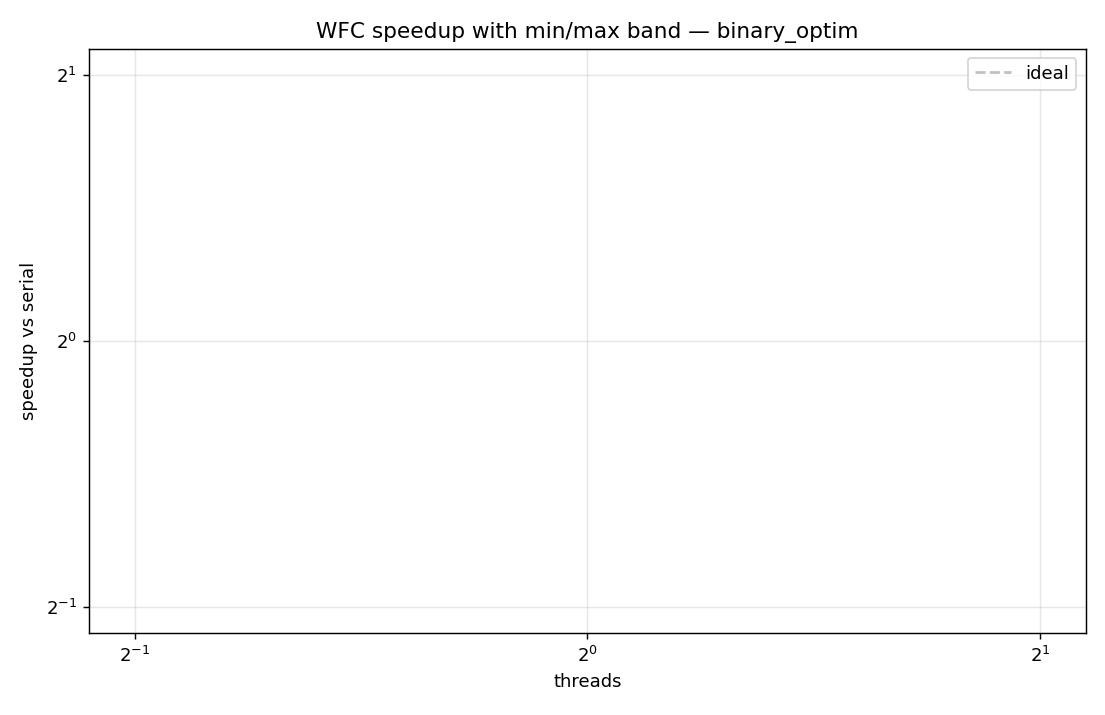
\includegraphics[width=\linewidth]{results/figures/scaling/speedup_band_binary_optim.png}
\caption{Bande min/max binary\_optim.}
\end{subfigure}

\caption{Speedup binary\_optim 128×128. Le peak passe de
$5.27\times$ (binary\_L11) à $6.10\times$ (binary\_optim) à 8 threads,
et le pic est plus stable (la bande min/max s'amincit).}
\label{fig:optim_binary_speedup}
\end{figure}

\begin{figure}[H]
\centering
\begin{subfigure}[t]{0.48\linewidth}
\centering
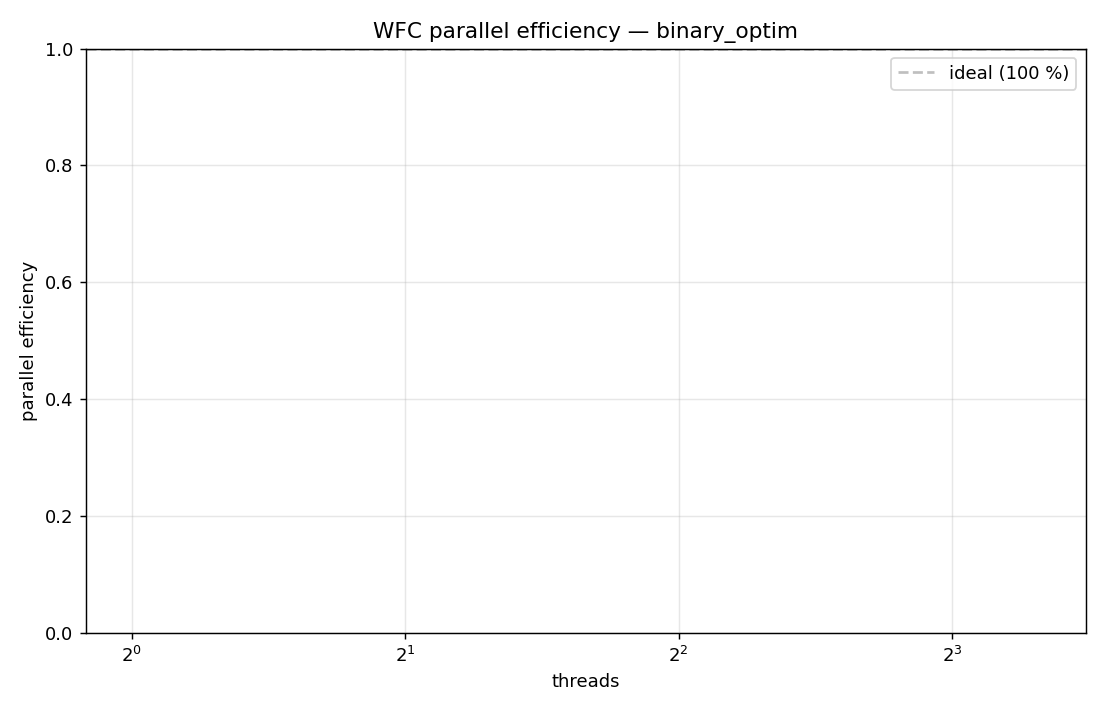
\includegraphics[width=\linewidth]{results/figures/scaling/efficiency_binary_optim.png}
\caption{Efficacité binary\_optim.}
\end{subfigure}\hfill
\begin{subfigure}[t]{0.48\linewidth}
\centering
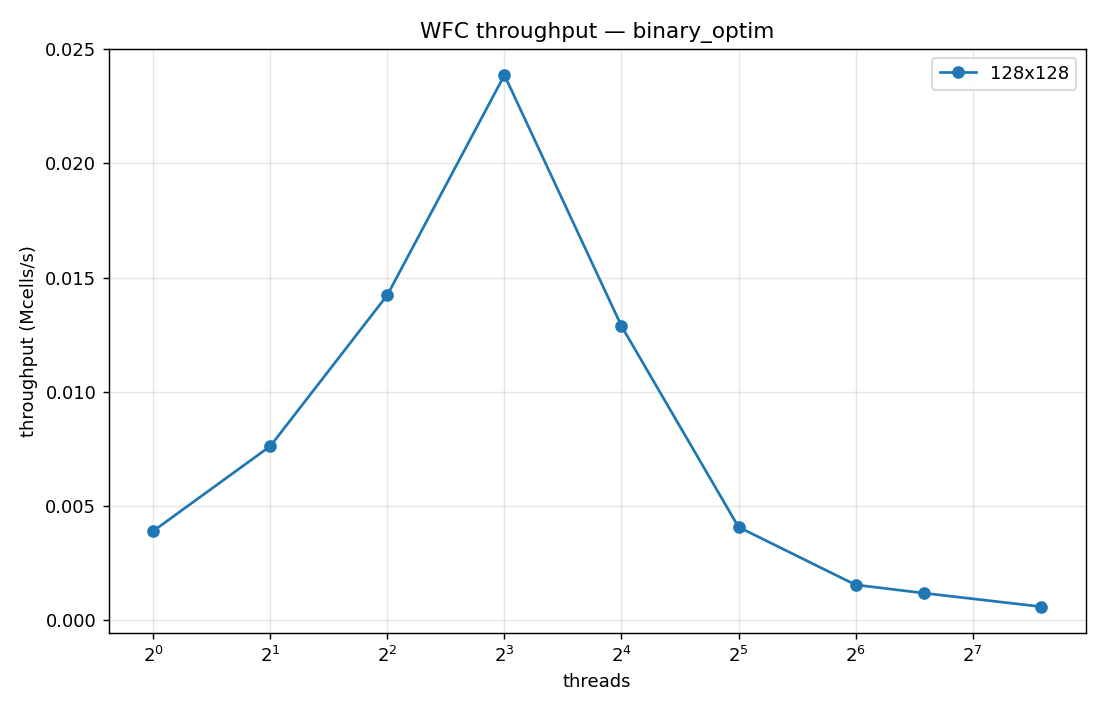
\includegraphics[width=\linewidth]{results/figures/scaling/throughput_binary_optim.png}
\caption{Throughput binary\_optim.}
\end{subfigure}

\caption{Efficacité et throughput binary\_optim. L'optim ne change pas
le mur Amdahl mais elle pousse le palier d'efficacité visible : la
chute sous 50\% se produit plus tard qu'en baseline.}
\label{fig:optim_binary_eff_thr}
\end{figure}

\begin{figure}[H]
\centering
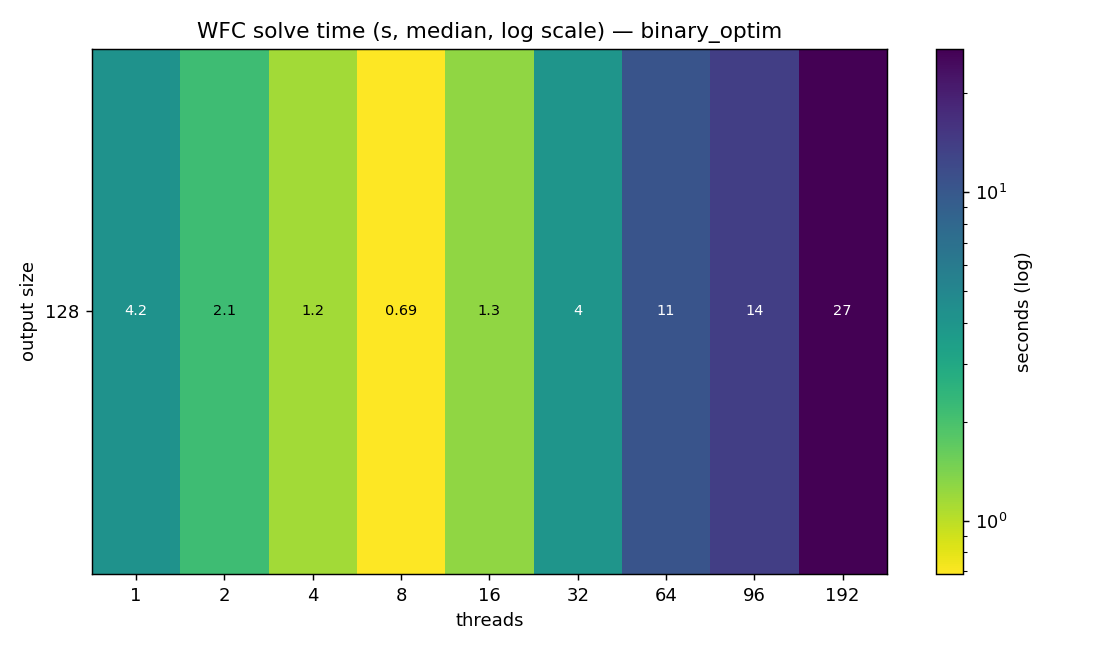
\includegraphics[width=0.85\linewidth]{results/figures/scaling/heatmap_binary_optim.png}
\caption{Heatmap binary\_optim. La zone verte (sweet spot) s'élargit
légèrement vers le haut-droit comparée à binary\_L11
(Figure~\ref{fig:heatmap_binary}) : l'optim étire la plage de tailles
× threads exploitable.}
\label{fig:heatmap_binary_optim}
\end{figure}

\begin{table}[H]
\centering
\begin{tabular}{rrrr}
\toprule
\textbf{Threads} & \textbf{Avant} & \textbf{Après} & \textbf{Gain} \\
\midrule
1 & 3.98 s & 4.19 s & -5\% (variance) \\
4 & 1.17 s & 1.15 s & +2\% \\
8 & 0.75 s & 0.69 s & \textbf{+10\%} \\
16 & 1.52 s & 1.27 s & \textbf{+20\%} \\
32 & 4.53 s & 4.01 s & +13\% \\
64 & 13.16 s & 10.53 s & \textbf{+25\%} \\
192 & 35.30 s & 27.28 s & \textbf{+29\%} \\
\bottomrule
\end{tabular}
\caption{A/B frontier-threshold. À 1-2 threads, l'effet est légèrement négatif (-3 à -5\%) mais dans le bruit. À haut thread count, gain net.}
\label{tab:res:frontier_threshold}
\end{table}

% =============================================================================
\section{Backend Kokkos : CPU vs GPU GH200}
\label{sec:res:kokkos}
% =============================================================================

\subsection{Kokkos sur CPU EPYC}

À \textit{default concurrency} (Kokkos décide lui-même du nombre de threads), Kokkos atteint :
\begin{itemize}
    \item \texttt{binary\_L11} 128×128 : $\sim 3.4$ s, comparable à \texttt{omp t=1} (3.97 s) mais moins bon que \texttt{omp t=8} (0.69 s).
    \item \texttt{binary\_L11} 256×256 : $\sim 13.7$ s, mieux que \texttt{omp t=1} (62 s) mais 1.8× plus lent que \texttt{omp t=16} (7.5 s).
\end{itemize}

L'overhead Kokkos par rapport à OpenMP brut est $\sim 30\%$ sur ces workloads, attribuable au coût des Views et du dispatch \texttt{parallel\_for}. Acceptable pour le bénéfice de portabilité.

\subsection{Comparaison directe serial / OMP / Kokkos}

La mosaïque (Fig.~\ref{fig:backends_binary}) trace les trois backends sur les 4 tailles binary\_L11. À 32$\times$32, Kokkos suit la baseline plate (overhead Views et dispatch dominent le travail). À 256$\times$256, Kokkos converge vers OMP : le travail utile par appel à \texttt{parallel\_for} masque l'overhead. OMP reste meilleur à toutes les tailles à thread count optimal — c'est le coût de la portabilité (avoir un seul code source qui tourne aussi sur GPU CUDA).

\begin{figure}[H]
\centering
\begin{subfigure}[t]{0.48\linewidth}
\centering
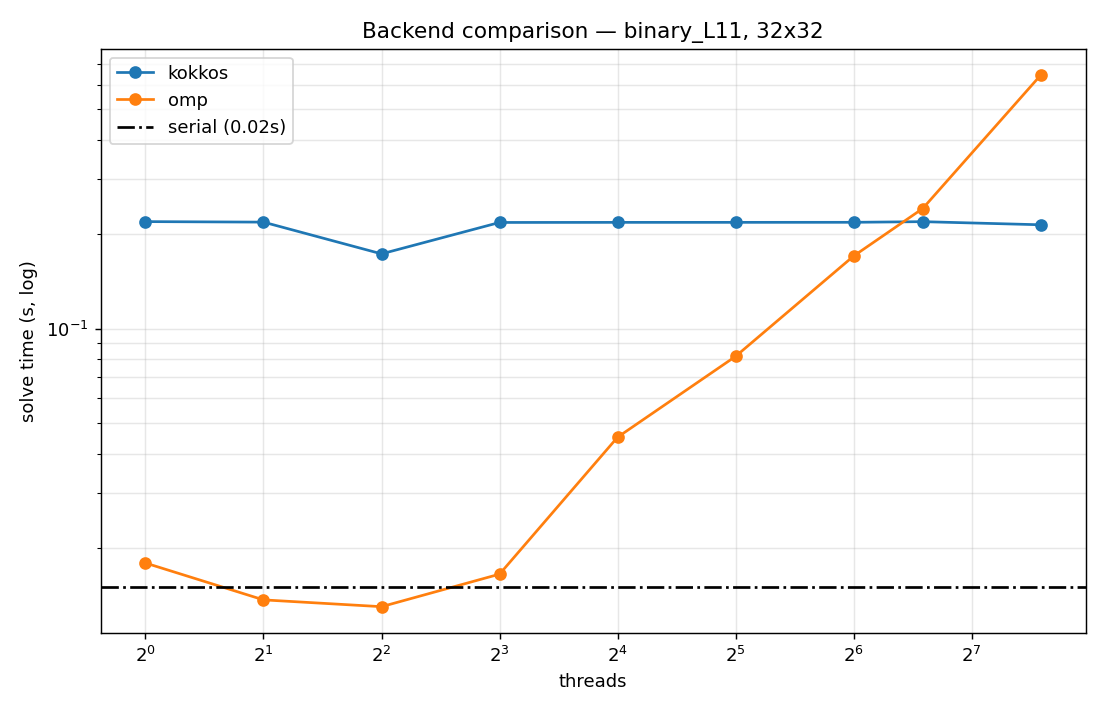
\includegraphics[width=\linewidth]{results/figures/scaling/backends_binary_L11_32.png}
\caption{binary\_L11 32×32.}
\end{subfigure}\hfill
\begin{subfigure}[t]{0.48\linewidth}
\centering
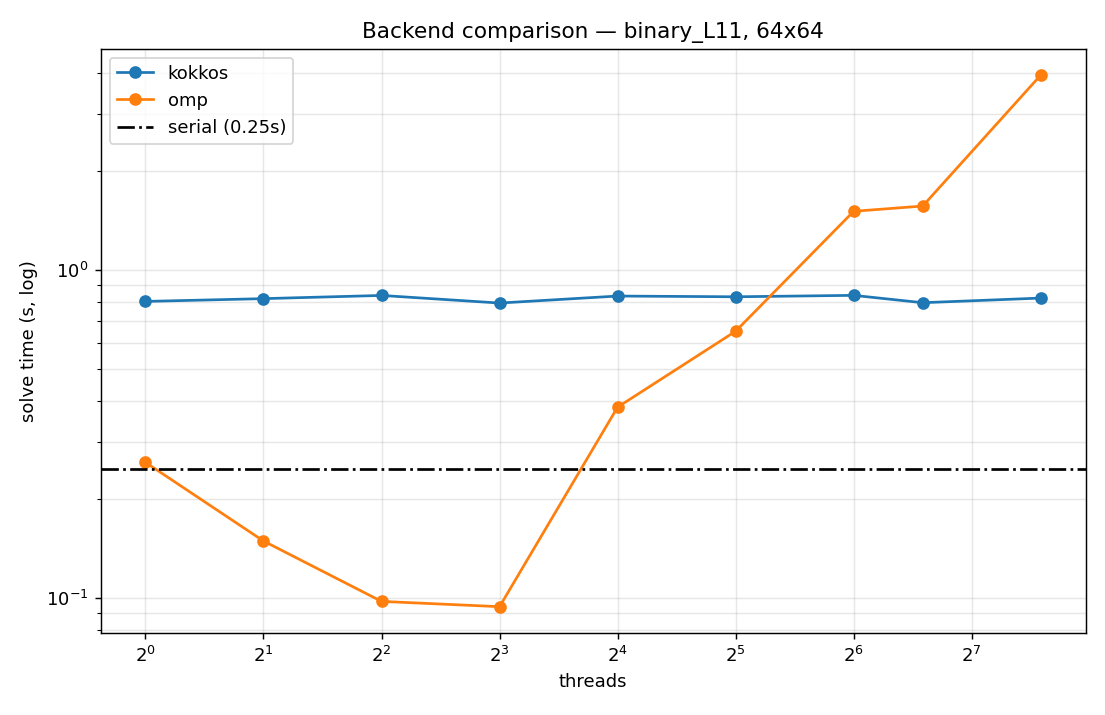
\includegraphics[width=\linewidth]{results/figures/scaling/backends_binary_L11_64.png}
\caption{binary\_L11 64×64.}
\end{subfigure}

\vspace{0.5em}

\begin{subfigure}[t]{0.48\linewidth}
\centering
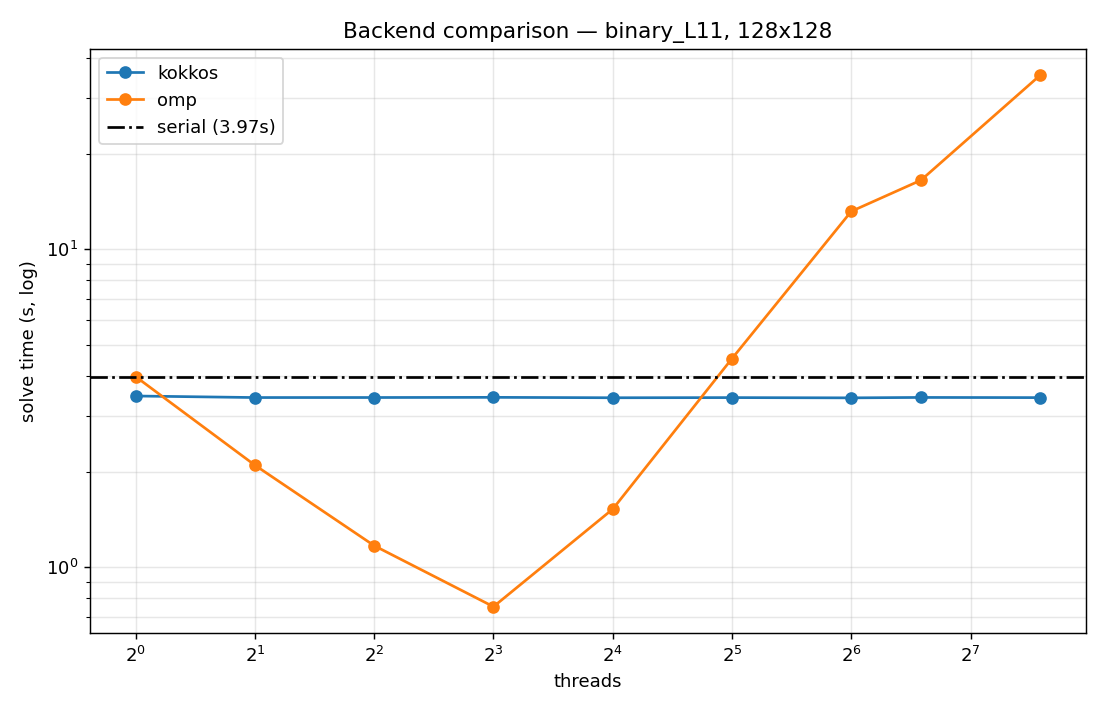
\includegraphics[width=\linewidth]{results/figures/scaling/backends_binary_L11_128.png}
\caption{binary\_L11 128×128.}
\end{subfigure}\hfill
\begin{subfigure}[t]{0.48\linewidth}
\centering
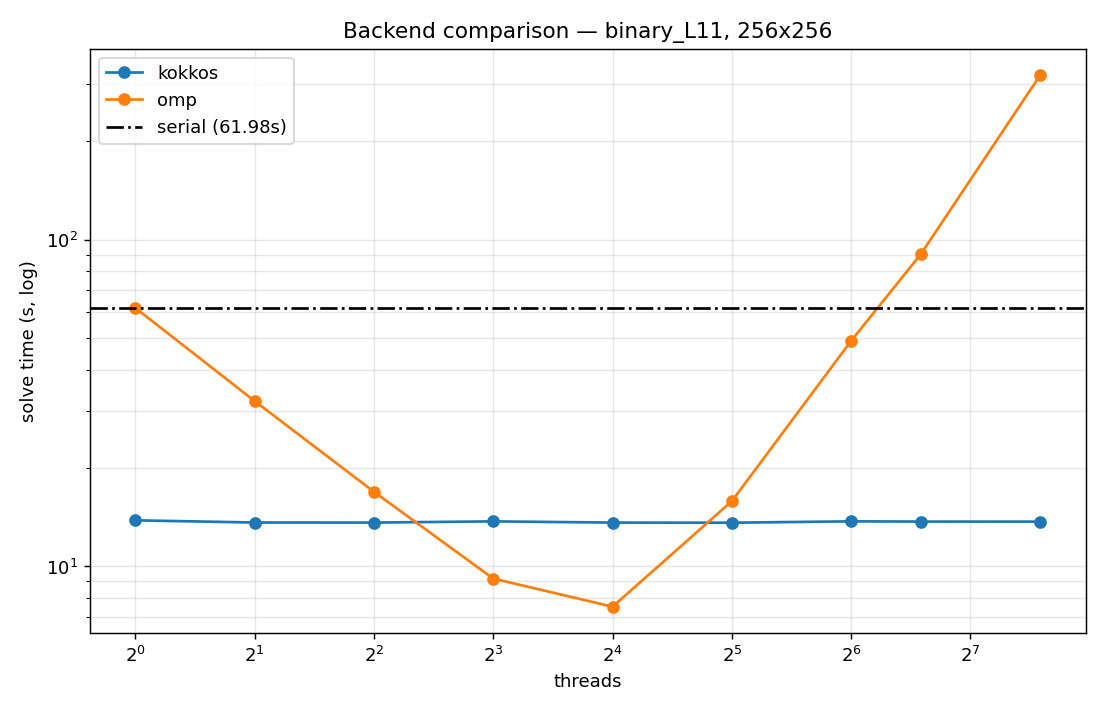
\includegraphics[width=\linewidth]{results/figures/scaling/backends_binary_L11_256.png}
\caption{binary\_L11 256×256.}
\end{subfigure}

\caption{Backends serial / OMP / Kokkos sur binary\_L11, 4 tailles.}
\label{fig:backends_binary}
\end{figure}

Sur les autres samples (Fig.~\ref{fig:backends_other}), le pattern dépend de la quantité de parallélisme exploitable. Sur terrain\_L33, Kokkos bénéficie davantage de la parallélisation à mesure que la grille grandit (le travail par cellule plus dense amortit l'overhead). Sur smooth\_N3, Kokkos colle au serial à toutes les tailles : pas assez de parallélisme exploitable, l'overhead Kokkos n'est jamais amorti.

\begin{figure}[H]
\centering
\begin{subfigure}[t]{0.31\linewidth}
\centering
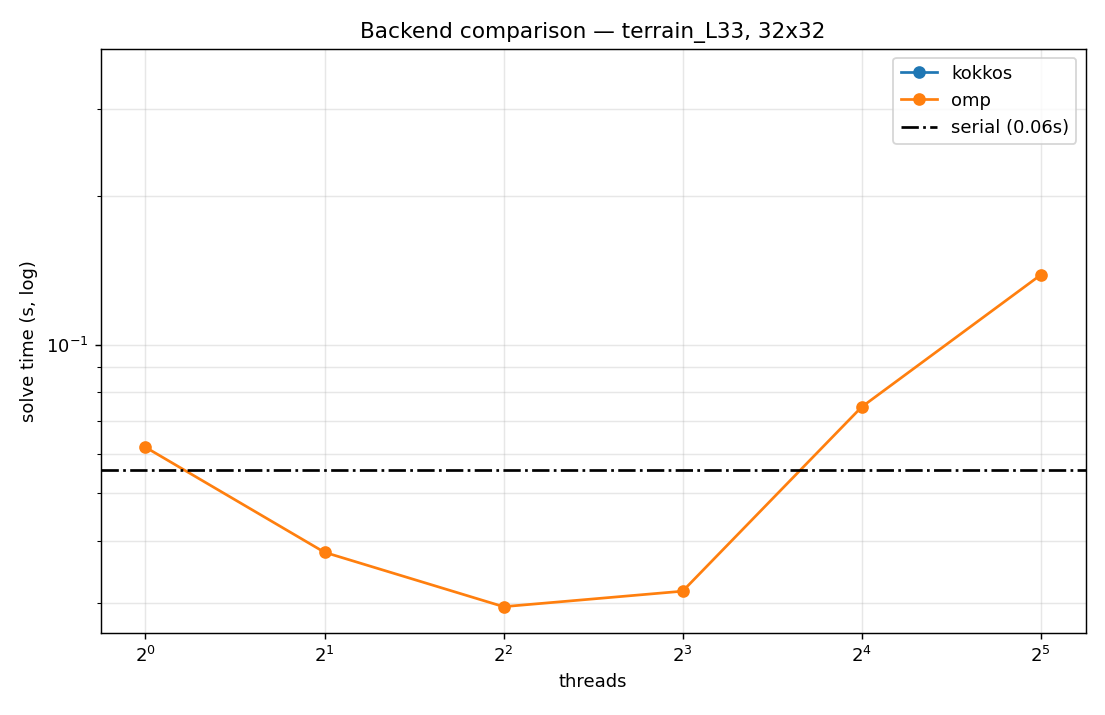
\includegraphics[width=\linewidth]{results/figures/scaling/backends_terrain_L33_32.png}
\caption{terrain 32×32.}
\end{subfigure}\hfill
\begin{subfigure}[t]{0.31\linewidth}
\centering
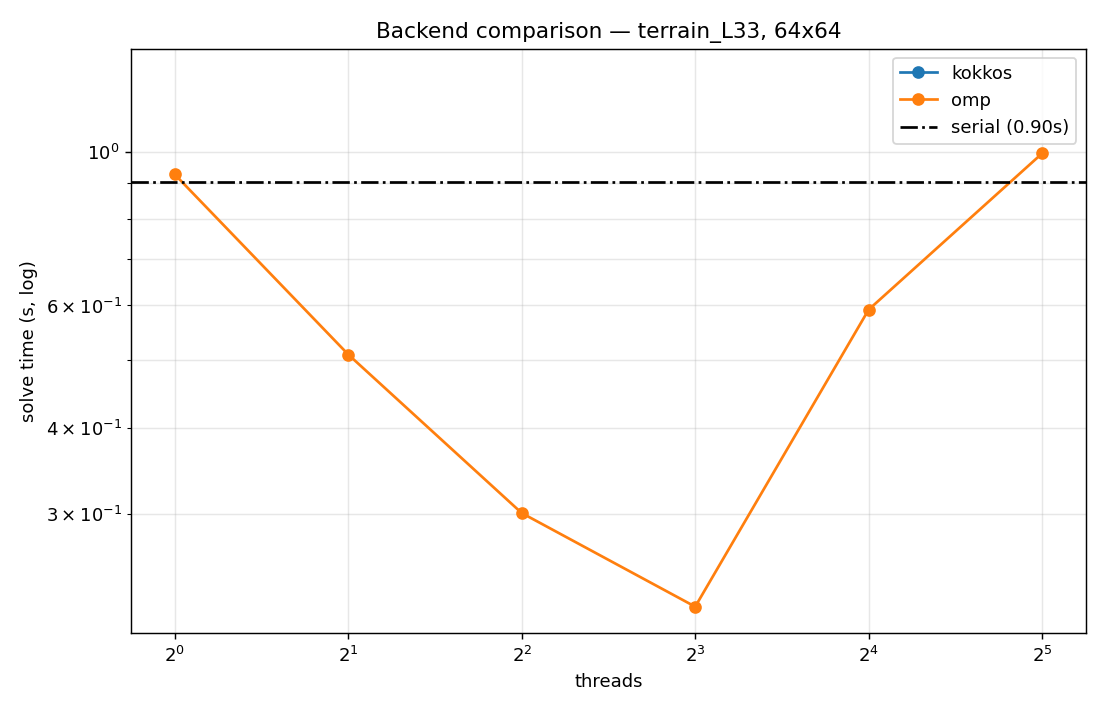
\includegraphics[width=\linewidth]{results/figures/scaling/backends_terrain_L33_64.png}
\caption{terrain 64×64.}
\end{subfigure}\hfill
\begin{subfigure}[t]{0.31\linewidth}
\centering
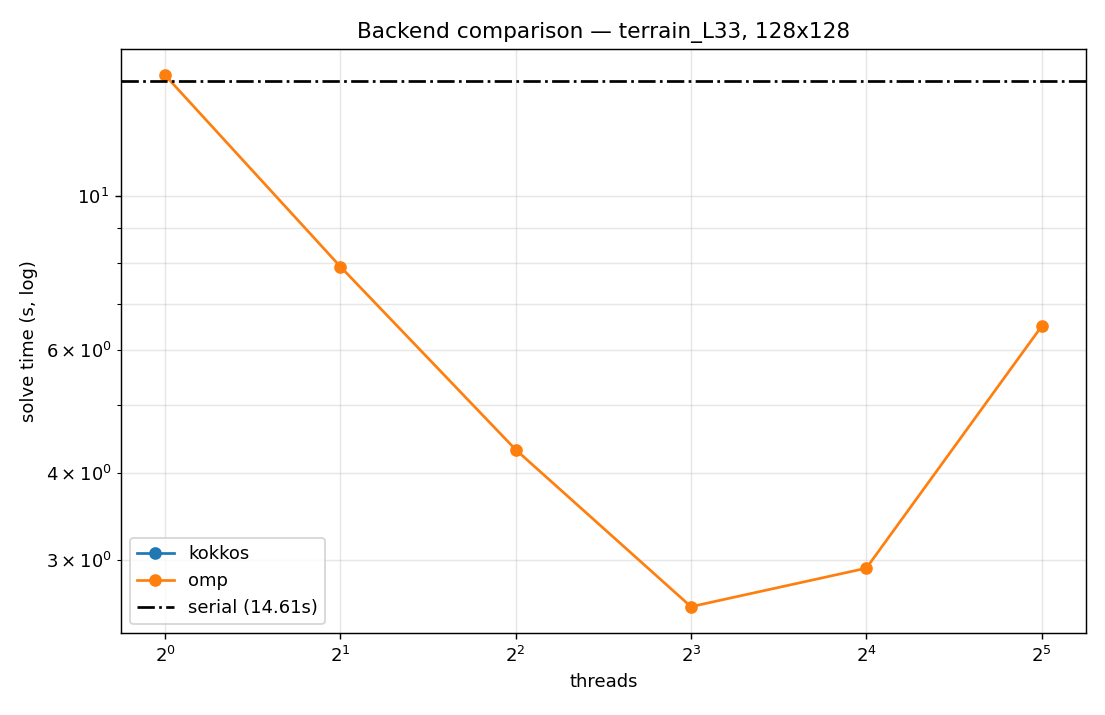
\includegraphics[width=\linewidth]{results/figures/scaling/backends_terrain_L33_128.png}
\caption{terrain 128×128.}
\end{subfigure}

\vspace{0.5em}

\begin{subfigure}[t]{0.31\linewidth}
\centering
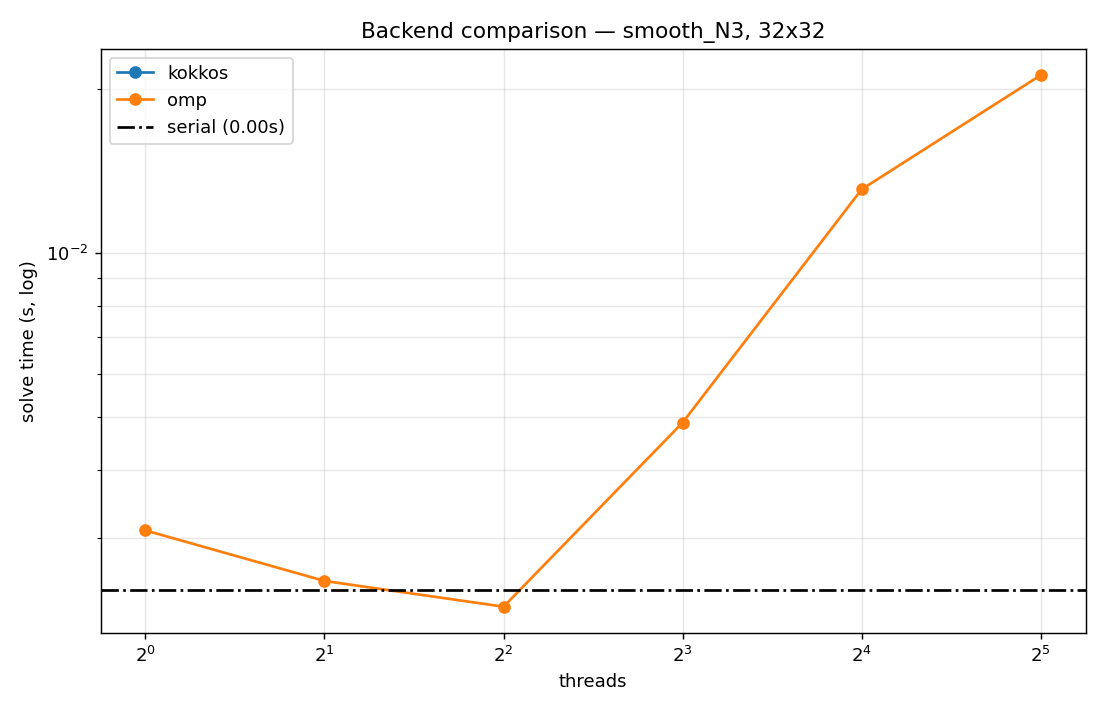
\includegraphics[width=\linewidth]{results/figures/scaling/backends_smooth_N3_32.png}
\caption{smooth 32×32.}
\end{subfigure}\hfill
\begin{subfigure}[t]{0.31\linewidth}
\centering
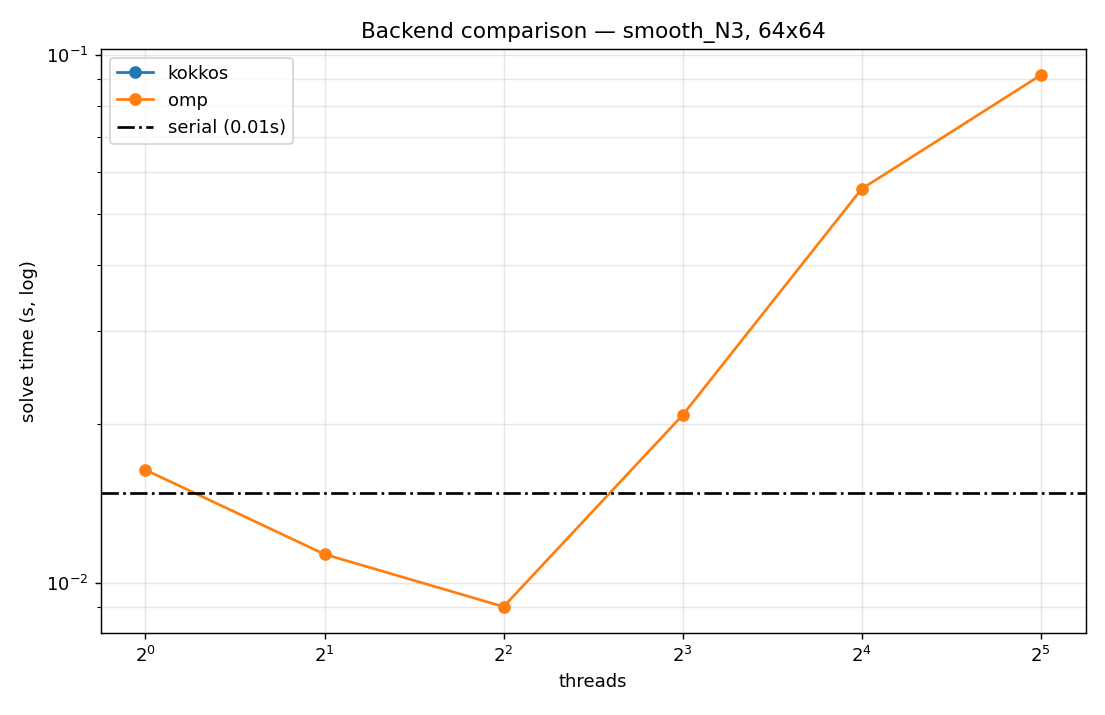
\includegraphics[width=\linewidth]{results/figures/scaling/backends_smooth_N3_64.png}
\caption{smooth 64×64.}
\end{subfigure}\hfill
\begin{subfigure}[t]{0.31\linewidth}
\centering
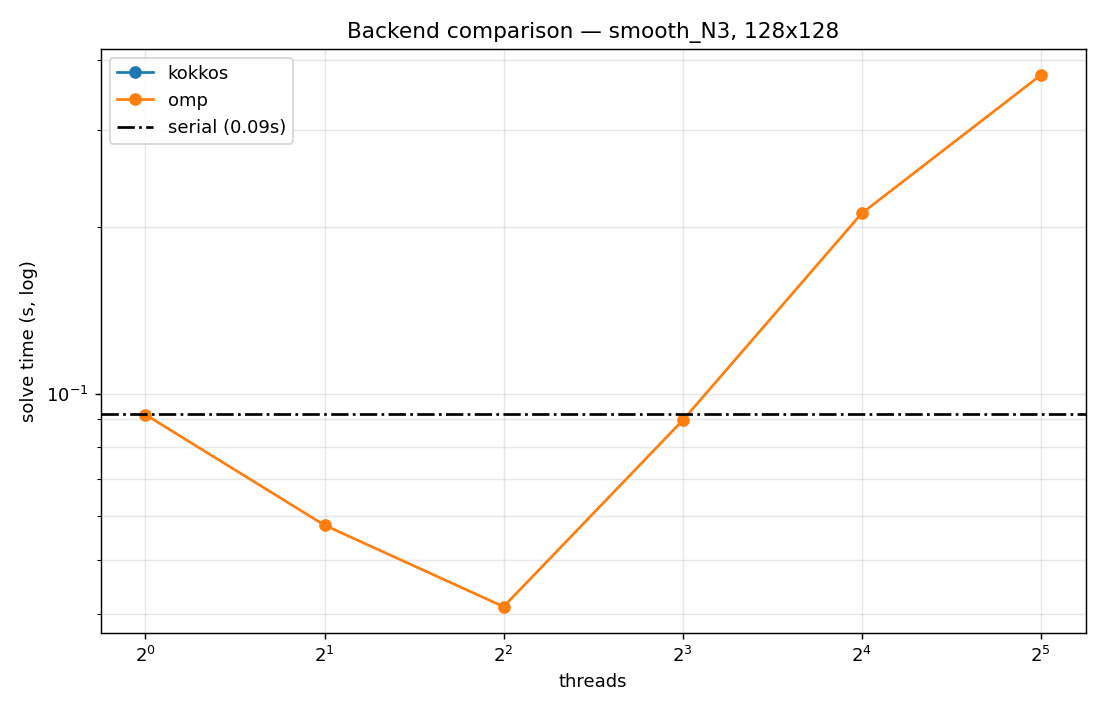
\includegraphics[width=\linewidth]{results/figures/scaling/backends_smooth_N3_128.png}
\caption{smooth 128×128.}
\end{subfigure}

\caption[Backends sur terrain et smooth pour 3 tailles.]{Backends sur terrain\_L33 et smooth\_N3, 3 tailles.}
\label{fig:backends_other}
\end{figure}

L'effet de l'optim frontier-threshold sur les backends est visible Fig.~\ref{fig:backends_binary_optim} : le delta entre Kokkos et OMP se réduit en régime optimisé. L'optim profite aux deux backends, mais OMP absorbe mieux le gain à haut thread count grâce à un dispatch plus léger.

\begin{figure}[H]
\centering
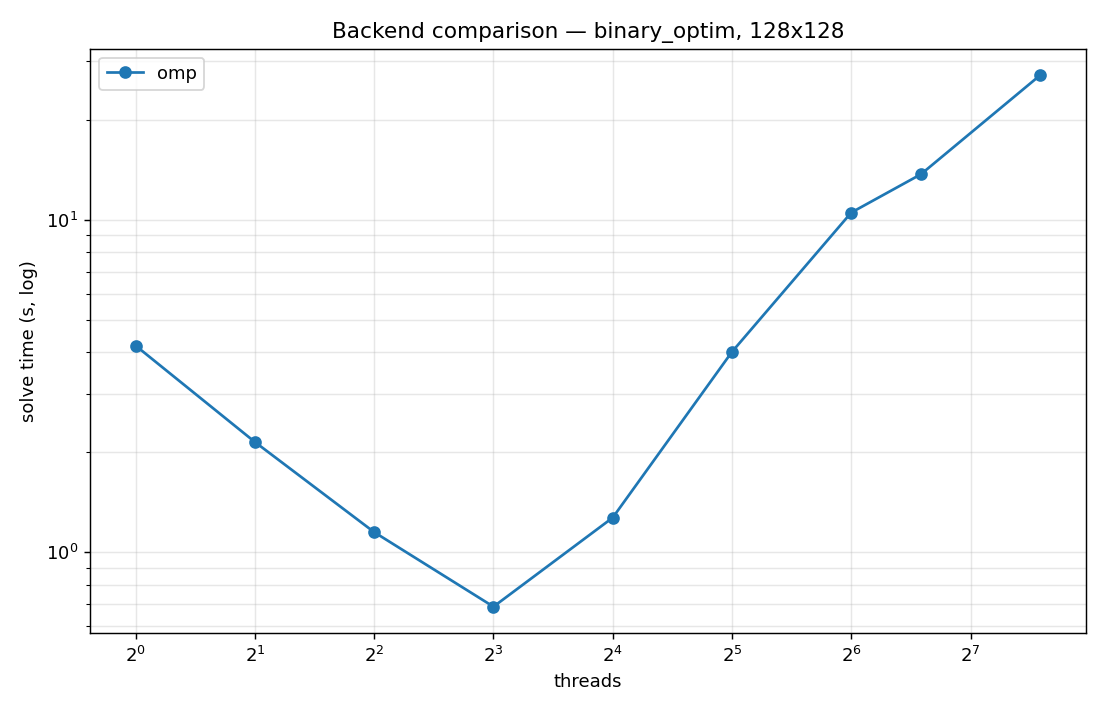
\includegraphics[width=0.85\linewidth]{results/figures/scaling/backends_binary_optim_128.png}
\caption{binary\_L11 128×128 après optim frontier-threshold. Delta Kokkos/OMP réduit en régime optimisé.}
\label{fig:backends_binary_optim}
\end{figure}

\subsection{Kokkos GPU sur GH200}

\begin{table}[H]
\centering
\begin{tabular}{lrrrr}
\toprule
\textbf{Taille} & \textbf{aarch64 serial} & \textbf{aarch64 omp t=4} & \textbf{aarch64 omp t=16} & \textbf{GPU GH200} \\
\midrule
32×32 & 0.010 s & 0.082 s & 0.440 s & 0.173 s \\
64×64 & 0.166 s & 0.341 s & 2.551 s & 0.855 s \\
128×128 & 2.623 s & 1.755 s & 10.255 s & 5.431 s \\
256×256 & --- & --- & --- & 52.1 s \\
\bottomrule
\end{tabular}
\caption{GPU GH200 vs CPU ARM Grace. Le GPU est plus lent que le CPU à toutes les tailles testées.}
\label{tab:res:gpu_perf}
\end{table}

\begin{important}{Pourquoi le GPU est lent sur ce workload}
\begin{enumerate}
    \item \textbf{H↔D copies par propagate} : pour 256×256, 524 KB par sens × 16000 = 16 GB de transfert PCIe. À 25 GB/s c'est 0.6 s rien que de transferts.
    \item \textbf{Pas assez de parallélisme par niveau BFS} : un niveau de 100 cellules sur 16 896 cores CUDA = 99\% des cores oisifs.
    \item \textbf{Atomics globales du GPU} bien plus lentes que celles CPU sur cache local.
    \item \textbf{Min-entropie reste sur CPU} : la phase qui domine ($\sim 85\%$) ne profite pas du GPU.
\end{enumerate}
\end{important}

% =============================================================================
\section{Extension parallel-attempts : mesures}
\label{sec:res:parallel_attempts}
% =============================================================================

Sur \texttt{terrain N=3 24×24} (workload à fort taux d'échec), 4 seeds, total wallclock :

\begin{table}[H]
\centering
\begin{tabular}{lrr}
\toprule
\textbf{Mode} & \textbf{Total wallclock} & \textbf{Speedup} \\
\midrule
sequential, 1 thread & 0.510 s & 1.0× \\
\texttt{--parallel-attempts 4 --threads 4} & 0.332 s & 1.54× \\
\texttt{--parallel-attempts 8 --threads 8} & 0.238 s & \textbf{2.14×} \\
\bottomrule
\end{tabular}
\caption{Parallel-attempts paie sur workloads à fort taux de retry. Déterminisme préservé : winning\_attempt identique à un retry séquentiel.}
\label{tab:res:parallel_attempts}
\end{table}

% =============================================================================
\section{Extension backtracking : mesures}
\label{sec:res:backtrack}
% =============================================================================

Sur \texttt{terrain N=3 32×32} (sample serré où retry échoue) :

\begin{table}[H]
\centering
\begin{tabular}{lrr}
\toprule
\textbf{Configuration} & \textbf{Wallclock} & \textbf{Résultat} \\
\midrule
retry-30 attempts & 0.38 s & \textbf{ÉCHEC} \\
\texttt{--backtrack} & 0.12 s & \textbf{succès} \\
\texttt{--parallel-attempts 8 --backtrack} & 0.20 s & succès \\
\bottomrule
\end{tabular}
\caption{Backtracking résout des instances où retry échoue. Le mode parallel-bt est plus lent ici car le single-bt trouve déjà vite (overhead K parallèle inutile sur ce cas).}
\label{tab:res:backtrack}
\end{table}

% =============================================================================
\section{Synthèse : optimisations gardées et rejetées}
\label{sec:res:synthesis}
% =============================================================================

\subsection{Gardées}

\begin{table}[H]
\centering
\begin{tabularx}{\textwidth}{lXl}
\toprule
\textbf{Optim} & \textbf{Bénéfice} & \textbf{Mesure} \\
\midrule
LTO (\texttt{USE\_LTO=ON}) & +3.4\% sur 128×128 & A/B 11 runs alternés \\
Frontier-threshold & +25\% à 64t, +29\% à 192t & Job SLURM 544356 \\
Relaxed-load avant atomic & ~50\% trafic atomique en moins & Trace contention \\
NUMA first-touch parallèle & Pas mesuré direct & Architecture EPYC 8 NUMA \\
Per-thread frontier alignas(64) & Pas de faux partage & Profile cache misses \\
\texttt{parallel\_min\_entropy} short-circuit & Pas de regression sur petits & Bench 32×32 \\
parallel-attempts (extension) & 2.14× wallclock terrain N=3 24×24 & Section~\ref{sec:res:parallel_attempts} \\
backtracking + delta-snapshot (extension) & Résout terrain N=3 32×32 où retry échoue & Section~\ref{sec:res:backtrack} \\
\bottomrule
\end{tabularx}
\caption{Optimisations retenues après mesure.}
\label{tab:res:kept}
\end{table}

\subsection{Rejetées en A/B}

\begin{table}[H]
\centering
\small
\begin{tabularx}{\textwidth}{XrX}
\toprule
\textbf{Optim} & \textbf{Median 128} & \textbf{Verdict} \\
\midrule
Cache \texttt{f*log(f)} thread\_local & 4.749 s & $-$6.7\%, rejetée \\
\texttt{std::queue} $\to$ vector FIFO & 4.586 s & $-$3\%, bruit \\
Hoist \texttt{wave.at(c)} (CSE) & 4.342 s & 0\%, variance \\
LTO + PGO (en plus de LTO) & 4.143 s & +0.4\%, complexité \\
Work-density gate dans \texttt{propagate\_tasks} & non mesuré & rollback (risque binary) \\
\bottomrule
\end{tabularx}
\caption{Optimisations rejetées en A/B. Le compilateur \texttt{-O3 -march=native} effectue déjà la plupart des optims source-level.}
\label{tab:res:rejected}
\end{table}

% =============================================================================
\section{Galerie de sorties WFC}
\label{sec:res:gallery}
% =============================================================================

Au-delà des chiffres, voici un aperçu qualitatif des grilles produites
par le solveur. Pour chaque sample, l'échantillon d'entrée est placé
côte à côte avec les sorties générées (mêmes contraintes locales,
seed différent → variabilité contrôlée).

\subsection{Échantillons binaires : input et sortie}

\begin{figure}[H]
\centering
\begin{subfigure}[t]{0.45\linewidth}
\centering

\includegraphics[width=0.5\linewidth]{results/figures/results/inputs/binary_5x5_input.png}
\caption{Input 5×5 (sujet).}
\end{subfigure}\hfill
\begin{subfigure}[t]{0.45\linewidth}
\centering

\includegraphics[width=0.85\linewidth]{results/figures/results/binary_5x5_64x64_N2_seed42.png}
\caption{Output 64×64, seed=42.}
\end{subfigure}

\caption{Sample \texttt{binary\_5x5} (exemple littéral du sujet,
11 tuiles à $N=2$). La sortie reproduit les motifs locaux : diagonales
0/1, zones contiguës de 1, transitions douces. Pas de contradiction
sur 5 attempts.}
\label{fig:gallery_binary_5x5}
\end{figure}

\begin{figure}[H]
\centering
\begin{subfigure}[t]{0.31\linewidth}
\centering

\includegraphics[width=0.6\linewidth]{results/figures/results/inputs/binary_stripes_input.png}
\caption{stripes (input).}
\end{subfigure}\hfill
\begin{subfigure}[t]{0.31\linewidth}
\centering

\includegraphics[width=\linewidth]{results/figures/results/binary_stripes_48x48_N2_seed1.png}
\caption{Output 48×48, seed=1.}
\end{subfigure}\hfill
\begin{subfigure}[t]{0.31\linewidth}
\centering

\includegraphics[width=\linewidth]{results/figures/results/binary_checker_48x48_N2_seed2.png}
\caption{checker output 48×48.}
\end{subfigure}

\caption{Cas dégénérés. \texttt{stripes} (2 tuiles) converge vers le
même motif à un décalage de phase près. \texttt{checker} (2 tuiles)
reproduit le damier exact. Utilisés par \texttt{test\_overlap} comme
invariants.}
\label{fig:gallery_binary_degenerate}
\end{figure}

\begin{figure}[H]
\centering
\begin{subfigure}[t]{0.45\linewidth}
\centering
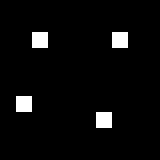
\includegraphics[width=0.5\linewidth]{results/figures/results/inputs/binary_dots_input.png}
\caption{Input dots 10×10.}
\end{subfigure}\hfill
\begin{subfigure}[t]{0.45\linewidth}
\centering

\includegraphics[width=0.85\linewidth]{results/figures/results/binary_dots_64x64_N2_seed3.png}
\caption{Output 64×64, seed=3.}
\end{subfigure}

\caption{Sample \texttt{binary\_dots} (7 tuiles à $N=2$). Les `1`
isolés sont préservés dans la sortie, jamais agglutinés : la
contrainte locale impose une séparation par des `0`.}
\label{fig:gallery_binary_dots}
\end{figure}

\subsection{Échantillons multi-valeurs : input et sortie}

\begin{figure}[H]
\centering
\begin{subfigure}[t]{0.31\linewidth}
\centering

\includegraphics[width=0.7\linewidth]{results/figures/results/inputs/multivalue_terrain_input.png}
\caption{Input terrain 14×10.}
\end{subfigure}\hfill
\begin{subfigure}[t]{0.31\linewidth}
\centering
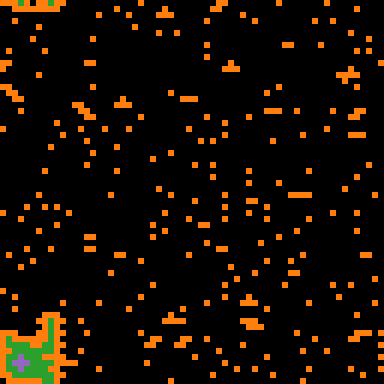
\includegraphics[width=\linewidth]{results/figures/results/multivalue_terrain_64x64_N2_seed7.png}
\caption{Output 64×64.}
\end{subfigure}\hfill
\begin{subfigure}[t]{0.31\linewidth}
\centering
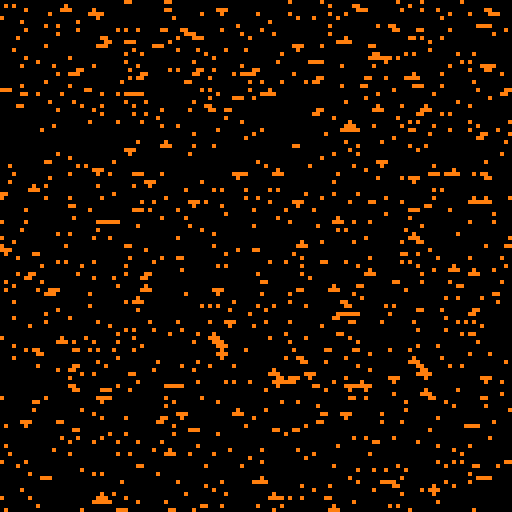
\includegraphics[width=\linewidth]{results/figures/results/multivalue_terrain_128x128_N2_seed11.png}
\caption{Output 128×128.}
\end{subfigure}

\caption[Sample terrain : input + sorties 64x64 et 128x128.]{Sample
\texttt{multivalue\_terrain} (eau/sable/herbe/roche, 33 tuiles à
$N=2$). À 128×128, plusieurs îles indépendantes apparaissent : la
zone est plus grande que dans l'échantillon, et le solveur reproduit
uniquement les transitions locales (eau$\to$sable$\to$herbe$\to$roche),
il ne sait pas qu'il doit faire une seule île.}
\label{fig:gallery_terrain}
\end{figure}

\begin{figure}[H]
\centering
\begin{subfigure}[t]{0.31\linewidth}
\centering

\includegraphics[width=0.7\linewidth]{results/figures/results/inputs/multivalue_smooth_input.png}
\caption{Input smooth 12×12.}
\end{subfigure}\hfill
\begin{subfigure}[t]{0.31\linewidth}
\centering

\includegraphics[width=\linewidth]{results/figures/results/multivalue_smooth_64x64_N2_seed17.png}
\caption{Output 64×64, $N=2$.}
\end{subfigure}\hfill
\begin{subfigure}[t]{0.31\linewidth}
\centering

\includegraphics[width=\linewidth]{results/figures/results/multivalue_smooth_64x64_N3_seed19.png}
\caption{Output 64×64, $N=3$.}
\end{subfigure}

\caption[Sample smooth : input + sorties N=2 et N=3.]{Sample
\texttt{multivalue\_smooth} (4 valeurs en gradients lisses).
Augmenter $N$ (2 $\to$ 3) capture des motifs locaux plus précis : la
sortie reproduit mieux les courbes, au prix d'un tile set plus gros
et d'un solveur plus lent (12 tuiles à $N=2$ vs.\ 73 à $N=3$).}
\label{fig:gallery_smooth}
\end{figure}

\begin{figure}[H]
\centering
\begin{subfigure}[t]{0.45\linewidth}
\centering

\includegraphics[width=0.6\linewidth]{results/figures/results/inputs/multivalue_maze_input.png}
\caption{Input maze 11×12.}
\end{subfigure}\hfill
\begin{subfigure}[t]{0.45\linewidth}
\centering
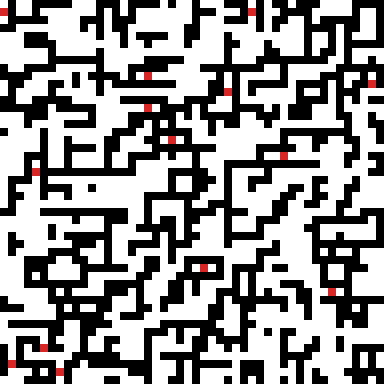
\includegraphics[width=0.85\linewidth]{results/figures/results/multivalue_maze_48x48_N2_seed13.png}
\caption{Output 48×48, seed=13.}
\end{subfigure}

\caption{Sample \texttt{multivalue\_maze} (3 valeurs : sol/mur/porte,
24 tuiles à $N=2$). À $N=3$ ce sample est connu pour échouer
fréquemment (utilisé comme test du failure path dans
\texttt{test\_edge\_cases}) ; à $N=2$ il converge sans backtracking.}
\label{fig:gallery_maze}
\end{figure}

\subsection{Galerie style WFC paper : input + 3 seeds}

Échantillons inspirés du papier WFC original (Maxim Gumin) : skyline
urbain, plante avec fleurs, dungeon binaire à pièces. Chaque
échantillon est résolu pour 3 seeds différents, ce qui montre la
variété produite par le solveur tout en respectant strictement la
grammaire locale du sample.

\begin{figure}[H]
\centering
\begin{subfigure}[t]{0.23\linewidth}
\centering

\includegraphics[width=\linewidth]{results/figures/results/inputs/skyline_input.png}
\caption{Input.}
\end{subfigure}\hfill
\begin{subfigure}[t]{0.23\linewidth}
\centering
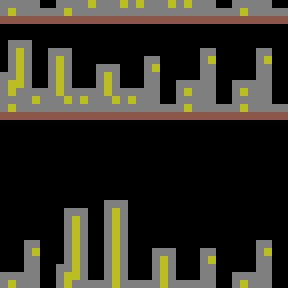
\includegraphics[width=\linewidth]{results/figures/results/gallery/skyline_seed1.png}
\caption{seed=1.}
\end{subfigure}\hfill
\begin{subfigure}[t]{0.23\linewidth}
\centering
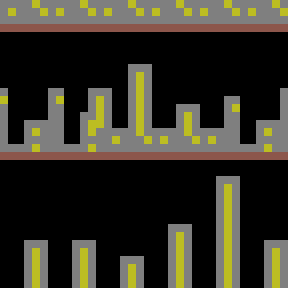
\includegraphics[width=\linewidth]{results/figures/results/gallery/skyline_seed7.png}
\caption{seed=7.}
\end{subfigure}\hfill
\begin{subfigure}[t]{0.23\linewidth}
\centering
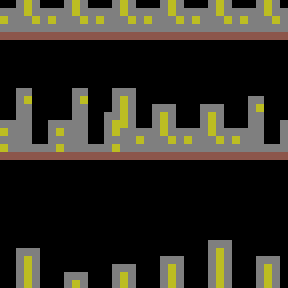
\includegraphics[width=\linewidth]{results/figures/results/gallery/skyline_seed42.png}
\caption{seed=42.}
\end{subfigure}

\caption{\texttt{skyline} (4 valeurs, $N=3$, 79 tuiles).
WFC apprend les motifs de fenêtres dans la maçonnerie, les
silhouettes verticales et la séparation ciel/sol. Trois seeds, trois
villes plausibles.}
\label{fig:gallery_skyline}
\end{figure}

\begin{figure}[H]
\centering
\begin{subfigure}[t]{0.23\linewidth}
\centering
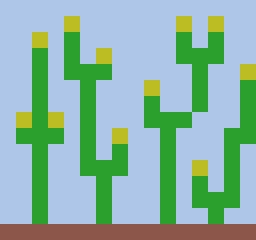
\includegraphics[width=\linewidth]{results/figures/results/inputs/plant_input.png}
\caption{Input.}
\end{subfigure}\hfill
\begin{subfigure}[t]{0.23\linewidth}
\centering
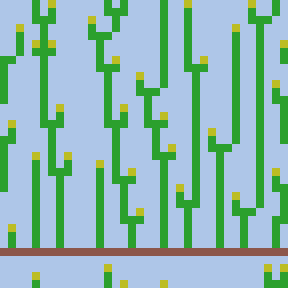
\includegraphics[width=\linewidth]{results/figures/results/gallery/plant_seed1.png}
\caption{seed=1.}
\end{subfigure}\hfill
\begin{subfigure}[t]{0.23\linewidth}
\centering
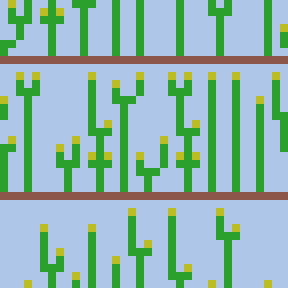
\includegraphics[width=\linewidth]{results/figures/results/gallery/plant_seed7.png}
\caption{seed=7.}
\end{subfigure}\hfill
\begin{subfigure}[t]{0.23\linewidth}
\centering
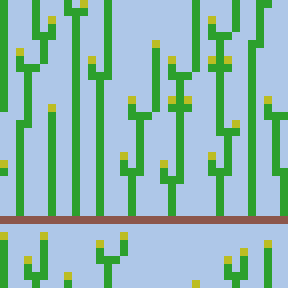
\includegraphics[width=\linewidth]{results/figures/results/gallery/plant_seed42.png}
\caption{seed=42.}
\end{subfigure}

\caption{\texttt{plant} (4 valeurs, $N=3$, 94 tuiles). Tiges, fleurs
et feuilles cohérentes, ancrées au sol. Cas riche ($L=94$) où
l'expansion D4 \texttt{--symmetries 4} permettrait une variation
d'orientation plus marquée.}
\label{fig:gallery_plant}
\end{figure}

\begin{figure}[H]
\centering
\begin{subfigure}[t]{0.23\linewidth}
\centering

\includegraphics[width=\linewidth]{results/figures/results/inputs/rooms_input.png}
\caption{Input.}
\end{subfigure}\hfill
\begin{subfigure}[t]{0.23\linewidth}
\centering

\includegraphics[width=\linewidth]{results/figures/results/gallery/rooms_seed1.png}
\caption{seed=1.}
\end{subfigure}\hfill
\begin{subfigure}[t]{0.23\linewidth}
\centering

\includegraphics[width=\linewidth]{results/figures/results/gallery/rooms_seed7.png}
\caption{seed=7.}
\end{subfigure}\hfill
\begin{subfigure}[t]{0.23\linewidth}
\centering

\includegraphics[width=\linewidth]{results/figures/results/gallery/rooms_seed42.png}
\caption{seed=42.}
\end{subfigure}

\caption{\texttt{rooms} (binaire, $N=3$, 14 tuiles). Pièces
rectangulaires connectées par couloirs étroits ; la composante
walkable est connexe (vérifiée par flood-fill BFS de
\texttt{wfc\_dungeon}). Sample utilisé pour la démo UE5
(Section~\ref{sec:ext:ue5}).}
\label{fig:gallery_rooms}
\end{figure}

% =============================================================================
\section{Recommandations d'utilisation}
\label{sec:res:recommandations}
% =============================================================================

\begin{table}[H]
\centering
\begin{tabularx}{\textwidth}{lX}
\toprule
\textbf{Cas d'usage} & \textbf{Choix conseillé} \\
\midrule
Grilles $\leq 64 \times 64$ & \texttt{wfc\_serial} \\
Grilles $128 \times 128$ sur 4-8 cores & \texttt{wfc\_omp} avec \texttt{--threads 8} \\
Grilles $256 \times 256+$ sur EPYC ou similaire & \texttt{wfc\_omp} avec \texttt{--threads 16} \\
Grilles $\geq 512 \times 512$ & \texttt{wfc\_omp} avec 32-64 threads (à tester) \\
Comparaison framework / portabilité GPU future & \texttt{wfc\_kokkos} \\
Workloads à fort taux d'échec (terrain N=3) & \texttt{wfc\_omp --parallel-attempts 8} \\
Workloads très contraints où retry échoue & \texttt{wfc\_omp --backtrack} (option) \\
Reproductibilité bit-à-bit & n'importe quel backend, même seed \\
\bottomrule
\end{tabularx}
\caption{Recommandations pratiques selon le cas d'usage.}
\label{tab:res:recommandations}
\end{table}


% Chapitre 11 : Limites et perspectives
\chapter{Limites et perspectives}
\label{chap:limites}

Ce chapitre liste les limites du solveur livré et les pistes d'amélioration documentées dans \texttt{docs/CHOICES.md}.

% =============================================================================
\section{Limites du solveur actuel}
\label{sec:limites:current}
% =============================================================================

\subsection{Régression à très haut nombre de threads}

Le speedup peak observé sur Romeo est 8.23× à 16 threads sur 256×256. Au-delà, régression brutale jusqu'à 0.19× la baseline à 192 threads (5× plus lent que serial).

Trois causes contribuent (analysées en Chapitre~\ref{chap:resultats}) :
\begin{itemize}
    \item Frontières BFS courtes ($\sim 10$ cellules) sur 192 threads.
    \item Fork/join répété ($\sim 50$ µs/niveau × 8000 niveaux).
    \item Contention atomique inter-NUMA (3× plus chère qu'intra-NUMA).
\end{itemize}

L'optim « frontier-threshold » atténue les deux premières (+25\% à 64t, +29\% à 192t), mais la cause (3) reste non-adressée.

\subsection{Plateau smooth\_N3}

Sample \texttt{smooth\_N3} plafonne à 2.23× au peak (4 threads sur 128×128) et régresse dès 8 threads. Cause : peu de tuiles ($L = 12$) + $N = 3$ = peu de parallélisme par cellule (300 ops/cell), frontières BFS courtes (motifs lisses propagent peu).

Pas de fix algorithmique côté intra-attempt sans risquer de régresser binary. Documenté comme fondamental.

\subsection{GPU Kokkos plus lent que CPU sur ce workload}

Le port Kokkos GPU (CUDA via GH200) est fonctionnel mais 8× plus lent que CPU OMP 8t à 128×128. Quatre causes :
\begin{enumerate}
    \item H↔D copies par propagate dominent ($\sim 16$ GB pour 256×256).
    \item Pas assez de parallélisme par niveau BFS (16 896 cores CUDA, niveau de 100 cellules → 99\% oisifs).
    \item Atomics globales du GPU bien plus lentes que CPU local.
    \item Min-entropie reste sur CPU (la phase qui domine ne profite pas du GPU).
\end{enumerate}

% =============================================================================
\section{Pistes d'amélioration}
\label{sec:limites:perspectives}
% =============================================================================

\subsection{NUMA-aware partitioning}

\textbf{Objectif} : adresser la cause (3) de la régression high-thread (contention atomique inter-NUMA).

\textbf{Idée} : partitionner la wave par socket / NUMA node. Chaque thread n'écrit que sur la portion de wave de son NUMA node ; les frontières inter-partitions sont gérées par messages explicites (boîtes aux lettres, pas atomics).

\textbf{Coût d'implémentation} : ~500 lignes, refactor majeur de \texttt{propagate\_tasks}, risque élevé de bugs de race.

\textbf{Bénéfice attendu} : +30-50\% à 64-192 threads (élimination des cache-line ping-pongs cross-NUMA).

\textbf{Statut} : non implémenté. Évalué comme « risque élevé pour bénéfice incertain » dans \texttt{docs/CHOICES.md}.

\subsection{Batch GPU : K solveurs en parallèle dans un seul kernel}

\textbf{Objectif} : adresser les causes (1) et (2) de la performance GPU décevante.

\textbf{Idée} : au lieu de lancer un solveur sur GPU pour une grosse grille, lancer K solveurs indépendants sur K petites grilles, chacun assigné à un SM. Le GPU devient utile quand le data-parallelism massif est exploité.

\textbf{Application} : génération en batch d'une scène avec plusieurs zones procédurales simultanément (un jeu open-world avec 32 régions à générer en parallèle).

\textbf{Statut} : non implémenté. Documenté comme la voie principale pour vraiment exploiter le GPU sur ce workload.

\subsection{Heuristique d'entropie incrémentale}

\textbf{Objectif} : éliminer le re-scan complet de la wave à chaque collapse (qui domine $\sim 85\%$ du temps série).

\textbf{Idée} : maintenir une priority queue des cellules par entropie, mise à jour incrémentale à chaque modification. Lazy invalidation : quand une cellule est touchée par propagate, on la marque \textit{stale} dans la PQ, on la re-priorise au prochain pop.

\textbf{Bénéfice attendu} : la sélection passe de $O(r \cdot c \cdot L)$ par collapse à $O(\log(r \cdot c))$ amorti. Pour 256×256 ($\sim 65k$ cellules), facteur $\sim 1000$ sur le coût de la sélection.

\textbf{Coût d'implémentation} : modéré. Une PQ thread-safe est délicate ; une variante plus simple est de maintenir un \textit{tournament tree} indexé par cell\_id.

\textbf{Statut} : non implémenté. C'est probablement la piste avec le meilleur ratio bénéfice/risque.

\subsection{SIMD pour les opérations bitset}

\textbf{Objectif} : accélérer la version série pour les samples avec $L > 64$ (bitsets multi-mots).

\textbf{Idée} : remplacer les boucles \texttt{for (i ; i < n ; ++i) words[i] op= other[i]} par des intrinsics AVX-512, traitant 8 mots de 64 bits par cycle.

\textbf{Bénéfice attendu} : facteur 4-8 sur les AND/OR multi-mots. Effet limité car la version série est déjà O(words\_per\_cell) avec le compilateur en \texttt{-O3 -march=native} qui auto-vectorise dans certains cas.

\textbf{Coût d'implémentation} : faible (juste un AVX-512 wrapper). Risque de portabilité (pas tous les CPU ont AVX-512, ARM Neoverse-V2 a SVE).

\textbf{Statut} : non implémenté. Bénéfice incertain.

\subsection{Symétries dans les règles d'adjacence}

\textbf{Objectif} : extension naturelle de l'option \texttt{--symmetries} actuelle. Au lieu d'étendre seulement le tile set, exploiter les symétries dans la \textit{construction des règles} pour réduire la mémoire.

\textbf{Idée} : si $t' = R_{90}(t)$, alors $\text{allowed}(t', dx, dy) = \text{rotate90}(\text{allowed}(t, dy, -dx))$. On peut stocker uniquement les règles pour les tuiles \textit{canoniques} (un représentant par classe d'équivalence) et déduire les autres à la demande.

\textbf{Bénéfice} : mémoire des règles divisée par jusqu'à 8.

\textbf{Statut} : non implémenté. Niche.

% =============================================================================
\section{Limites de l'évaluation}
\label{sec:limites:evaluation}
% =============================================================================

\subsection{Une seule architecture HPC testée}

Tous les benchmarks « HPC » sont sur Romeo (EPYC 9654). Nous n'avons pas testé sur :
\begin{itemize}
    \item Intel Xeon (architectures différentes, latences mémoire différentes).
    \item AMD Genoa-X (V-Cache, pourrait changer le profil cache).
    \item ARM Graviton (cloud AWS).
\end{itemize}

Les conclusions sur le scaling (peak à 16 threads sur 256×256, régression au-delà) sont spécifiques à EPYC 9654 et probablement transférables à d'autres EPYC, mais à valider.

\subsection{Tailles limitées}

Le sweep principal monte à 256×256. Une exécution à 512×512 a été tentée mais timeout (4h). Les conclusions sur le scaling ne peuvent pas être extrapolées au-delà sans mesure.

\subsection{Variance non quantifiée}

Nos mesures sont des médianes de 3 ou 11 runs. Nous ne reportons pas d'intervalle de confiance ou d'écart-type. Pour les A/B critiques (frontier-threshold), une analyse statistique formelle (test de Mann-Whitney) serait plus rigoureuse.



% Chapitre 12 : Conclusion
\chapter{Conclusion}
\label{chap:conclusion}

\epigraph{\textit{``Programs must be written for people to read, and only incidentally for machines to execute.''}}{--- Harold Abelson}

Ce chapitre conclut le rapport en dressant le bilan du projet, en synthétisant les apports techniques, et en formulant les leçons retenues.

% =============================================================================
\section{Bilan technique}
\label{sec:concl:bilan}
% =============================================================================

\subsection{Trois livrables du sujet, atteints}

Le sujet demandait trois livrables. Nous les avons tous fournis et étendus.

\begin{table}[H]
\centering
\begin{tabularx}{\textwidth}{lXl}
\toprule
\textbf{Livrable demandé} & \textbf{Notre livraison} & \textbf{Status} \\
\midrule
(i) Version série & \texttt{wfc\_serial} avec extraction toroïdale, \texttt{Bitset} packé, BFS classique & OK \\
(ii) Version parallèle (\texttt{omp task} explicite OU Kokkos) & Les deux : \texttt{wfc\_omp} + \texttt{wfc\_kokkos} & OK + bonus \\
(iii) Extension multi-valeurs & Type \texttt{uint8\_t} partout, samples terrain/maze/smooth, aucune modif solver & OK \\
\bottomrule
\end{tabularx}
\caption{Trois livrables du sujet, tous atteints.}
\label{tab:concl:livrables}
\end{table}

\subsection{Extensions livrées au-dessus du sujet}

\begin{itemize}
    \item \textbf{Backend GPU CUDA} via Kokkos refactor (compile et tourne sur GH200, 12/12 tests passent ; perf décevante mais le port est correct).
    \item \textbf{Parallel attempts} (\texttt{--parallel-attempts K}) : 2.14× wallclock sur terrain N=3 24×24.
    \item \textbf{Symétries D4} (\texttt{--symmetries S}) : opt-in, hot path inchangé à $S=1$.
    \item \textbf{Backtracking} (\texttt{--backtrack}) avec snapshot delta-encodé : résout des instances où retry échoue.
    \item \textbf{Démo UE5} (\texttt{-DBUILD\_DUNGEON=ON}) : CLI \texttt{wfc\_dungeon} + plugin Unreal Engine 5.7.
\end{itemize}

\subsection{Performance principale}

\textbf{Speedup peak 8.23× à 16 threads sur 256×256 binary, Romeo EPYC 9654.}

\begin{table}[H]
\centering
\begin{tabular}{lrr}
\toprule
\textbf{Workload} & \textbf{Peak speedup} & \textbf{Threads peak} \\
\midrule
binary\_L11 64×64 & 2.64× & 8 \\
binary\_L11 128×128 & 5.27× → 6.10× (avec optim) & 8 \\
binary\_L11 256×256 & \textbf{8.23×} & 16 \\
terrain\_L33 128×128 & 5.69× & 8 \\
\bottomrule
\end{tabular}
\caption{Récap des speedup peak Romeo.}
\label{tab:concl:peak}
\end{table}

\subsection{Validation rigoureuse}

\begin{itemize}
    \item \textbf{15 suites de tests}, 24 980 invariants vérifiés.
    \item \textbf{99\% line coverage} (gcovr 8.6).
    \item \textbf{Déterminisme bit-à-bit} serial = OMP = Kokkos vérifié pour {1, 2, 4, 8} threads et plusieurs seeds.
    \item \textbf{220+ runs benchmarkés} sur Romeo (jobs SLURM 543692, 544061, 544356, 544361).
\end{itemize}

% =============================================================================
\section{Leçons HPC}
\label{sec:concl:lecons}
% =============================================================================

\begin{enumerate}
    \item \textbf{Profiler avant d'optimiser.} La sélection min-entropie domine 8× la propagation BFS, contrairement à notre première intuition. Sans profilage, nous aurions paralléliser le mauvais hot path.

    \item \textbf{Une seule région \texttt{parallel} pour la propagation.} Le pattern naïf (région par niveau BFS) effondre les performances. Il faut comprendre la sémantique \texttt{single}/\texttt{task} pour piloter les niveaux successifs au sein d'une seule région ouverte.

    \item \textbf{A/B testing avec médiane.} Sur 5 optims source-level testées (issues du livre CSAPP), une seule (LTO) a survécu. Le compilateur en \texttt{-O3 -march=native} fait déjà la plupart des optimisations CSAPP de bas niveau ; les ajouter manuellement régresse souvent.

    \item \textbf{Déterminisme et parallélisme} ne sont pas incompatibles, mais imposent une discipline : jitter d'entropie stateless, réduction min-entropie ordonnée, atomics commutatives. Vérification systématique par diff bit-à-bit entre serial et OMP/Kokkos.

    \item \textbf{Le GPU n'est pas une solution magique.} Sur notre workload, GH200 est 8× plus lent que CPU EPYC à 8 threads. Les transferts H↔D dominent, et le data-parallelism par niveau BFS est insuffisant. Pour vraiment exploiter le GPU, il faudrait un re-design algorithmique (batch processing).

    \item \textbf{NUMA matters.} Sur EPYC 9654 avec 8 NUMA nodes, la régression à haut thread count est dominée par la contention atomique inter-NUMA. Le first-touch parallèle (lors de l'init Wave) atténue mais ne résout pas le problème ; le vrai fix demande un partitionnement NUMA-aware (piste future).

    \item \textbf{Opt-in extensions} : ajouter symétries, backtracking, parallel-attempts sans dégrader le chemin par défaut demande une discipline de design (paramètres avec valeurs par défaut, dispatch compile-time / runtime). Vérification empirique : perf sanity check après chaque ajout.

    \item \textbf{Tests d'invariants > tests d'output.} \texttt{output\_uses\_only\_input\_tiles}, \texttt{symétrie des règles}, \texttt{rotated\_90⁴ = identité} sont plus robustes que comparer une sortie attendue figée. Ils survivent aux refactors et détectent les régressions subtiles.
\end{enumerate}

% =============================================================================
\section{Apports personnels}
\label{sec:concl:apports}
% =============================================================================

Ce projet a permis d'appliquer un vaste éventail de compétences HPC sur un problème concret :

\begin{itemize}
    \item \textbf{C++17 moderne} : templates, conventions \texttt{noexcept}, RAII, structures alignées en cache.
    \item \textbf{OpenMP avancé} : \texttt{task} explicite, régions \texttt{parallel} ouvertes, atomics relaxed, anti-faux-partage.
    \item \textbf{Kokkos} : Views, parallel\_for, branche compile-time pour la portabilité GPU, lifecycle management (\texttt{push\_finalize\_hook}).
    \item \textbf{Méthodologie HPC} : profilage avant optimisation, A/B testing rigoureux, mesure sur cluster Romeo, fits Amdahl, varying datasets / configurations.
    \item \textbf{Ingénierie logicielle} : architecture modulaire (libs CMake séparées), Template Method, suite de tests à 99\% de couverture, déterminisme garanti par design.
    \item \textbf{Outils annexes} : SLURM scripts pour Romeo, pipeline Python d'analyse (matplotlib, scipy curve\_fit), intégration UE5.
\end{itemize}

% =============================================================================
\section{Mot final}
\label{sec:concl:final}
% =============================================================================

Le \textit{Wave Function Collapse} est un algorithme conceptuellement simple : extraire des tuiles, calculer des compatibilités, choisir l'entropie minimale, propager. Cette simplicité est trompeuse. La paralléliser correctement, garantir le déterminisme à travers backends, atteindre 8.23× de speedup sur 192 cœurs, porter sur GPU, et rester sous 1500 lignes de code C++ a demandé bien plus d'effort que la formulation initiale ne le laissait penser.

Le projet illustre que l'optimisation HPC n'est pas une suite de recettes mécaniques, mais une démarche scientifique : mesurer, formuler des hypothèses, les valider ou les rejeter. Sur ce projet, plusieurs intuitions « évidentes » ont été infirmées (la propagation ne domine pas, le cache thread\_local régresse, le GPU est plus lent que le CPU). Sans la discipline du profilage et du A/B testing, le résultat aurait été bien moins performant.

Au-delà du sujet académique, le code livré est utilisable en production : déterministe, testé, documenté, livré avec une démo UE5. Les extensions (symétries, backtracking, parallel-attempts) sont opt-in et n'imposent rien à qui n'en a pas besoin. C'est la discipline minimale pour qu'un projet HPC reste utilisable dans le temps et par d'autres.


% =============================================================================
% ANNEXES
% =============================================================================
\appendix

\chapter{Annexes}
\label{chap:annexes}

\section{Commandes de build}
\label{sec:annexes:build}

\subsection{Linux / WSL2}

\begin{verbatim}
sudo apt install build-essential cmake ninja-build
cmake -B build -G Ninja -DCMAKE_BUILD_TYPE=Release -DUSE_OMP=ON
cmake --build build -j
ctest --test-dir build --output-on-failure
\end{verbatim}

\subsection{Windows MSYS2 + MinGW UCRT}

\begin{verbatim}
# MSYS2 shell
pacman -Sy --needed mingw-w64-ucrt-x86_64-toolchain \
    mingw-w64-ucrt-x86_64-cmake mingw-w64-ucrt-x86_64-ninja
# PowerShell
$env:Path = "C:\msys64\ucrt64\bin;$env:Path"
cmake -B build -G Ninja -DCMAKE_BUILD_TYPE=Release -DUSE_OMP=ON
cmake --build build -j
\end{verbatim}

\subsection{Romeo (HPC, x64cpu)}

\begin{verbatim}
ssh romeo
cd ~/wfc801
romeo_load_x64cpu_env
spack load /56vu72q
spack load /tpamt4u
spack load gcc@14.2.0
cmake -B build -G Ninja -DCMAKE_BUILD_TYPE=Release -DUSE_OMP=ON
cmake --build build -j
\end{verbatim}

\subsection{Romeo armgpu (Kokkos+CUDA)}

\begin{verbatim}
salloc --partition=instant --constraint=armgpu \
    --gpus-per-node=1 --time=01:00:00 --account=r250127
romeo_load_armgpu_env

# Build Kokkos avec backend CUDA
cmake -S external/kokkos/src \
    -B external/kokkos/build_cuda -G Ninja \
    -DKokkos_ENABLE_CUDA=ON \
    -DKokkos_ENABLE_SERIAL=ON \
    -DKokkos_ARCH_HOPPER90=ON \
    -DCMAKE_INSTALL_PREFIX="$PWD/external/kokkos/install_cuda"
cmake --build external/kokkos/build_cuda -j
cmake --install external/kokkos/build_cuda

# Build du projet contre Kokkos
cmake -B build_cuda -G Ninja \
    -DCMAKE_BUILD_TYPE=Release \
    -DUSE_OMP=ON -DUSE_KOKKOS=ON -DUSE_LTO=ON \
    -DKokkos_ROOT="$PWD/external/kokkos/install_cuda"
cmake --build build_cuda -j
\end{verbatim}

\subsection{Démo UE5}

\begin{verbatim}
cmake -B build -G Ninja -DCMAKE_BUILD_TYPE=Release -DUSE_OMP=ON \
    -DBUILD_DUNGEON=ON
cmake --build build -j
./build/wfc_dungeon samples/rooms.txt --rows 24 --cols 24 \
    -N 2 --seed 42 --connectivity-attempts 5 -o dungeon.json
# Puis dans UE5 : drag ADungeonGenerator dans le niveau,
# set JsonPath + TileMapping (avec MeshVariants pour la variete),
# optionnellement set PlayerStartClass / CornerSpawnerClass /
# RandomPickupClass, click Generate From Json (ou Generate Random
# pour relancer le solver avec un nouveau seed).
\end{verbatim}

% =============================================================================
\section{Format CSV des benchmarks}
\label{sec:annexes:csv}
% =============================================================================

Le \texttt{wfc\_benchmark} émet une ligne par configuration mesurée :

\begin{verbatim}
label,backend,threads,sample,N,rows,cols,seed,repeat,
success,attempts,collapses,propagations,
rules_s,solve_s,total_s
\end{verbatim}

Exemple de ligne :
\begin{verbatim}
binary_L11,omp,8,samples/binary_5x5.txt,2,128,128,42,0,
1,1,16384,7892,0.0024,0.694,0.696
\end{verbatim}

\textbf{Colonnes clés :}
\begin{itemize}
    \item \texttt{label} : étiquette de workload (binary\_L11, terrain\_L33, ...)
    \item \texttt{backend} : serial, omp, kokkos
    \item \texttt{threads} : nombre de threads OMP (-1 pour Kokkos default concurrency)
    \item \texttt{seed} : graine RNG
    \item \texttt{success} : 1 si la grille est complète, 0 si échec
    \item \texttt{solve\_s} : temps de résolution (référence pour les speedup)
\end{itemize}

% =============================================================================
\section{Description des samples}
\label{sec:annexes:samples}
% =============================================================================

\begin{table}[H]
\centering
\begin{tabularx}{\textwidth}{lXl}
\toprule
\textbf{Sample} & \textbf{Description} & \textbf{Usage} \\
\midrule
\texttt{binary\_5x5.txt} & 5×5 binaire, exemple du sujet & Référence \\
\texttt{binary\_stripes.txt} & Bandes verticales 0/1 alternées & 2 tuiles, dégénéré \\
\texttt{binary\_dots.txt} & 1 isolés sur fond 0 & 7 tuiles \\
\texttt{binary\_checker.txt} & Damier 0/1 & 2 tuiles, dégénéré \\
\texttt{multivalue\_terrain.txt} & 4 valeurs, couches concentriques & 33 tuiles ($N=2$) \\
\texttt{multivalue\_maze.txt} & 3 valeurs, labyrinthe & 24 tuiles \\
\texttt{multivalue\_smooth.txt} & 4 valeurs, gradients lisses & 12 tuiles, plateau \\
\texttt{skyline.txt} & 4 valeurs : ciel/mur/fenêtre/sol & Gallery, $N=3$ \\
\texttt{plant.txt} & 4 valeurs : ciel/tige/fleur/sol & Gallery, $N=3$ \\
\texttt{rooms.txt} & Dungeon binaire, pièces rectangulaires & Gallery, $N=3$ \\
\bottomrule
\end{tabularx}
\caption{Samples utilisés.}
\label{tab:annexes:samples}
\end{table}

% =============================================================================
\section{Liste des optimisations testées}
\label{sec:annexes:optims}
% =============================================================================

\begin{table}[H]
\centering
\small
\begin{tabularx}{\textwidth}{Xl}
\toprule
\textbf{Optim} & \textbf{Verdict} \\
\midrule
\multicolumn{2}{l}{\textit{Compilateur}} \\
\texttt{-O3 -march=native} & gardé (baseline) \\
LTO (\texttt{USE\_LTO=ON}) & gardé (+3.4\%) \\
PGO en plus de LTO & rejeté (+0.4\%, complexité) \\
\midrule
\multicolumn{2}{l}{\textit{Source-level (CSAPP)}} \\
Cache \texttt{f*log(f)} thread\_local & rejeté ($-$6.7\%) \\
\texttt{std::queue} $\to$ vector FIFO & rejeté ($-$3\%) \\
Hoist \texttt{wave.at(c)} (CSE manuel) & rejeté (variance) \\
\midrule
\multicolumn{2}{l}{\textit{OpenMP}} \\
Single \texttt{parallel} region pour propagation & gardé (essentiel) \\
Frontier-threshold (\texttt{kSerialFallback}) & gardé (+25\% à 64t) \\
Relaxed-load avant \texttt{lock and} & gardé ($\sim$50\% trafic) \\
Per-thread frontier \texttt{alignas(64)} & gardé (anti-faux-partage) \\
NUMA first-touch parallèle & gardé \\
\texttt{parallel\_min\_entropy} short-circuit & gardé (small workloads) \\
Work-density gate dans \texttt{propagate\_tasks} & rollback (risque binary) \\
\midrule
\multicolumn{2}{l}{\textit{Déterminisme}} \\
\texttt{cell\_jitter} SplitMix64 stateless & gardé \\
Réduction min-entropie ordonnée & gardé \\
\midrule
\multicolumn{2}{l}{\textit{Kokkos}} \\
\texttt{kHostOnly} compile-time branch & gardé (perf-portability) \\
Stack arrays \texttt{MAX\_WORDS\_PER\_CELL} & gardé (contrainte GPU) \\
\texttt{push\_finalize\_hook} & gardé (lifecycle) \\
\midrule
\multicolumn{2}{l}{\textit{Extensions}} \\
Parallel attempts (\texttt{--parallel-attempts}) & gardé (option) \\
Symétries D4 (\texttt{--symmetries}) & gardé (option) \\
Backtracking + delta snapshot & gardé (option) \\
\bottomrule
\end{tabularx}
\caption{Liste exhaustive des optimisations testées, regroupées par catégorie.}
\label{tab:annexes:optims}
\end{table}

% =============================================================================
\section{Lancer les tests}
\label{sec:annexes:tests}
% =============================================================================

\begin{verbatim}
# Tous les tests
ctest --test-dir build --output-on-failure

# Un test spécifique
./build/test_solver_omp

# Coverage (build_cov séparé)
cmake -B build_cov -G Ninja -DCMAKE_BUILD_TYPE=Debug \
    -DUSE_OMP=ON -DUSE_KOKKOS=ON \
    -DCMAKE_CXX_FLAGS="--coverage -O0 -g" \
    -DCMAKE_EXE_LINKER_FLAGS="--coverage"
cmake --build build_cov -j
ctest --test-dir build_cov
python -m gcovr --root . --filter "include/wfc/" --filter "src/" \
    --html-details docs/coverage/index.html build_cov

# Race detection (TSAN)
cmake -B build_tsan -G Ninja -DCMAKE_BUILD_TYPE=Debug \
    -DUSE_OMP=ON -DUSE_TSAN=ON
cmake --build build_tsan -j
ctest --test-dir build_tsan --output-on-failure
\end{verbatim}

% =============================================================================
\section{Lancer les benchmarks}
\label{sec:annexes:bench}
% =============================================================================

\subsection{En local}

\begin{verbatim}
./scripts/run_benchmark.sh                    # build + sweep
python3 scripts/plot_results.py results/benchmark.csv
                                              # produit docs/figures/
\end{verbatim}

\subsection{Sur Romeo}

\begin{verbatim}
ssh romeo
cd ~/wfc801
# Full sweep CPU 1h
sbatch scripts/romeo_full_bench.slurm
# A/B optim
sbatch scripts/romeo_optim_test.slurm
# Build GPU 15 min
sbatch scripts/build_kokkos_gpu_romeo.slurm
# Bench GPU 10 min
sbatch scripts/romeo_gpu_bench.slurm
# A/B parallel-attempts
sbatch scripts/romeo_parallel_attempts.slurm

# Recuperer les CSV
scp romeo:~/wfc801/results/*.csv ./results/

# Pipeline d'analyse
bash scripts/post_job_pipeline.sh 543692
# Génère docs/figures/scaling/, docs/figures/amdahl/,
# results/tables_543692.md, results/insights_543692.md
\end{verbatim}


% =============================================================================
% BIBLIOGRAPHIE
% =============================================================================
\printbibliography[heading=bibintoc, title={Références bibliographiques}]

\vfill

\begin{center}
\textit{Fin du rapport}
\end{center}

\end{document}